%!TEX TS-program = xelatex %!TEX encoding = UTF-8 Unicode
\documentclass{zc-thesis}
%\usepackage{draftwatermark}          %use these two lines for draft
%\SetWatermarkText{DRAFT}\SetWatermarkScale{1}\SetWatermarkColor[rgb]{0.9,0.5,0.5}

\begin{document}
\hypersetup{pdfauthor={Zhang, Chao},    pdfcopyright={Copyright (C) 2017 by Zhang, Chao.
    Licensed under CC-BY-SA 4.0. Some rights reserved.},
    pdflicenseurl={https://creativecommons.org/licenses/by-sa/4.0/}} 
% some details about the thesis
\title{Probing Nanomaterial Properties in a High-resolution Transmission Electron Microscope}

\author{Chao Zhang}
\advisor{Dmitri Golberg}

% about the degree
\degree{Doctor of Philosophy}
\field{Materials Science and Engineering}
\degreeyear{2017}
\degreemonth{February}

% about the university
\department{Pure and Applied Sciences}
\university{University of Tsukuba}
\universitycity{Tsukuba}
\universitystate{Ibaraki}
\maketitle 
\copyrightpage\dedicationpage\abstractpage\acknowledgments\tableofcontents
\onehalfspacing\listoffigures\listoftables \afterpage{\null\newpage}
\pagestyle{fancy}\fancyhf{}
\fancyhead[RE]{\scriptsize \nouppercase \rightmark}
\fancyhead[LO]{\scriptsize \nouppercase \leftmark}
\fancyfoot[LE]{{\LARGE \bf \thepage} \hspace{15pt} 
.....................................................................................................................................................................}
\fancyfoot[RO]{
..................................................................................................................................................................... \hspace{15pt} {\LARGE \bf \thepage}}

\setlength{\textfloatsep}{10pt plus 1.0pt minus 2.0pt}  %floats length
\setlength{\floatsep}{10.0pt plus 1.0pt minus 2.0pt}
\setlength{\intextsep}{10.0pt plus 1.0pt minus 2.0pt}

%update: Jan 13 fixed grammar according to prof notes
%update: Jan 09-11 prof check
%update: Dec 20 finish writing
%update: Nov 09 Prof checked some of the texts

%\begin{savequote}[75mm] 
%There's plenty of room at the bottom.
%\qauthor{Richard Feynman} 
%\end{savequote}

\chapter{Introduction}

\newthought{The advancement of materials science and technology} has led to the discovery and utilization of nanoscale materials. Many of these new materials possess extraordinary chemical, electrical, optical or mechanical properties. However, as human beings, who are millions or billions times larger than nanomaterials, we are not perfectly scaled to reach them directly. As Feynman said, there is plenty of room at the bottom, but it also means that plenty of efforts are expected toward researching. 

\begin{figure} 
\centering
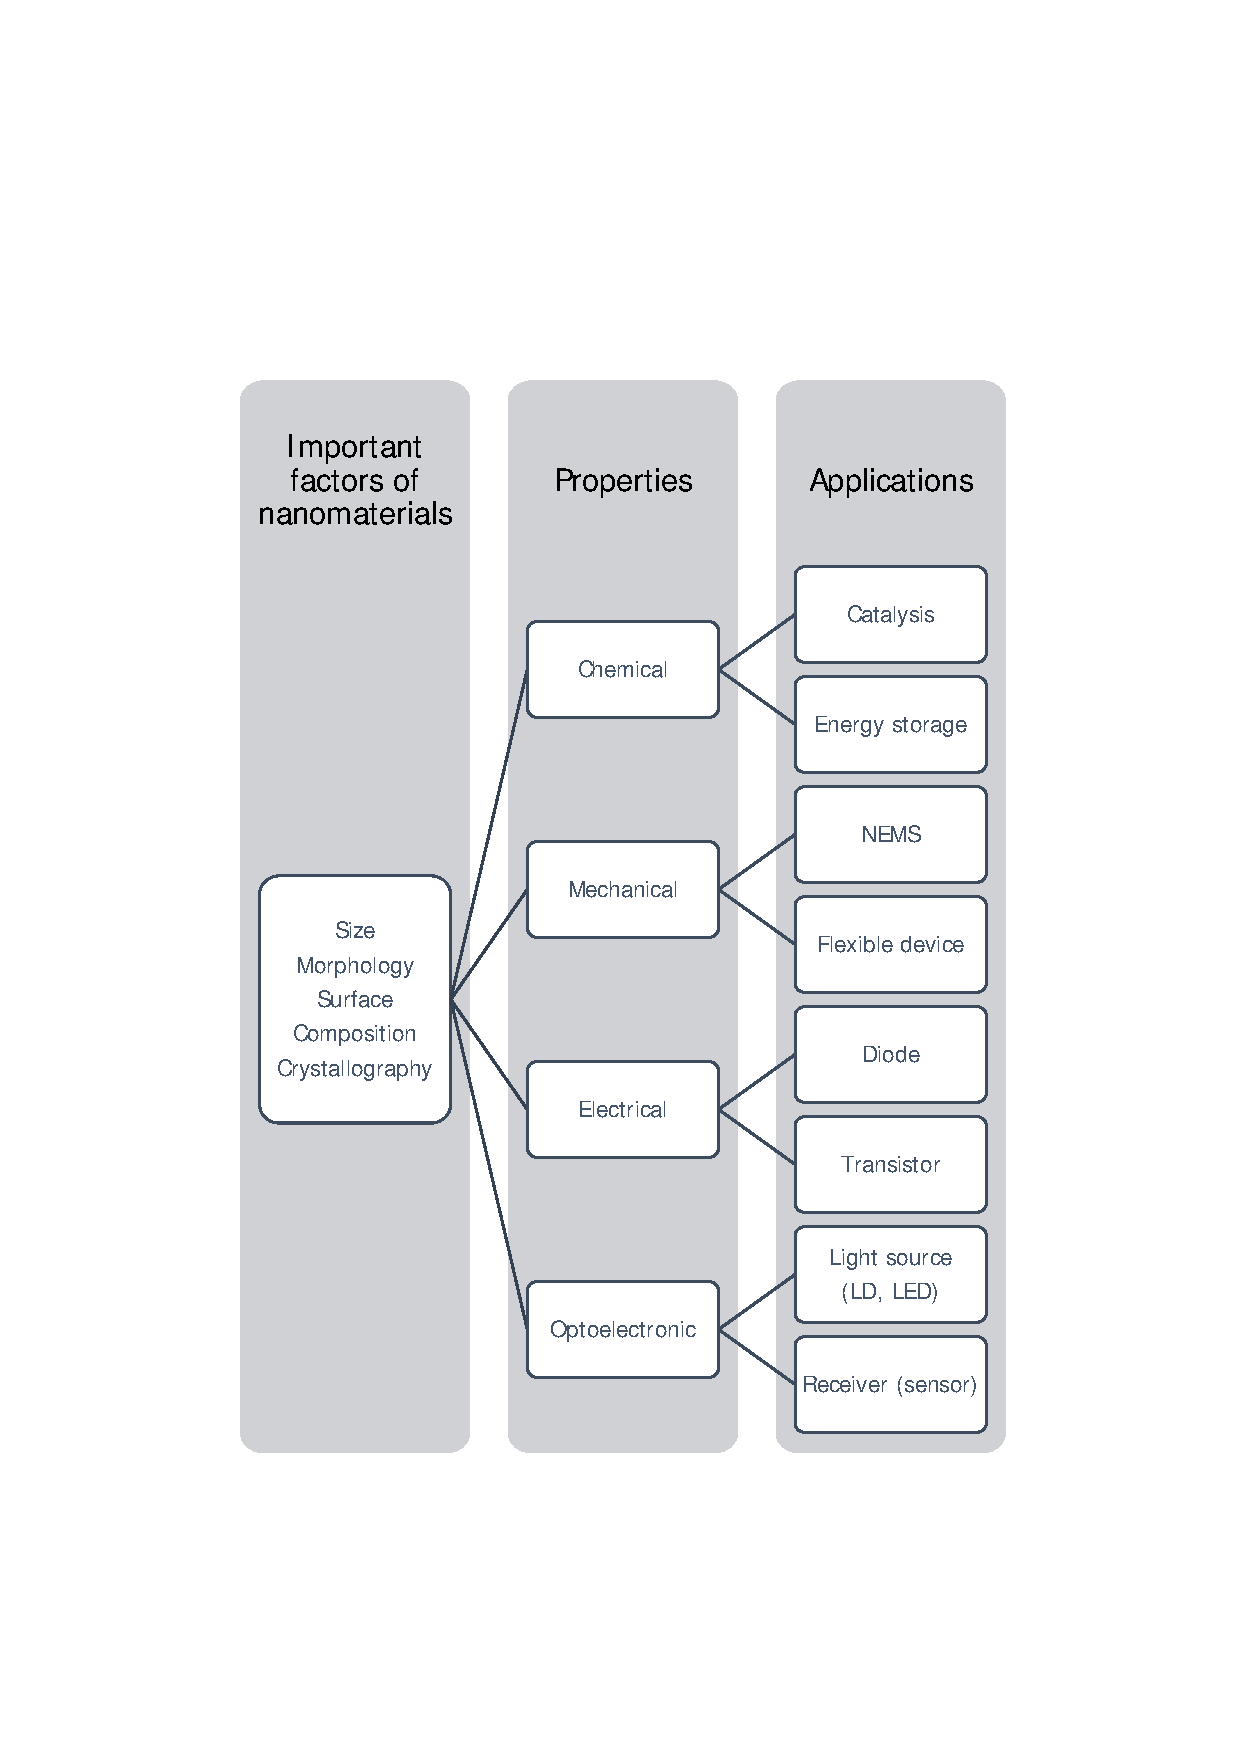
\includegraphics[width=400pt]{figures/figure1_factors}
\caption[Factors and applications]{Special factors of nanomaterials contributing to various applications. 
\label{fig:1_factor}}
\end{figure}

%nanoscale--nanomaterials--to see--to manipulate
\section{Probing of nanomaterials}
%what is nanomater...why nanomater...
Generally, nanomaterials are materials in which a single unit is sized from one nanometer to a few hundred nanometers. The scale difference between these materials and human body is more than a million. Besides scale difference, nanostructures usually possess special properties as compared with bulk materials due to chemical composition difference, surface to volume ratio and quantum confinements. The confined structures of the same chemical type and composition might present very different properties. An easy way to understand a value of the nanomaterial is to consider carbon materials. We know diamond and graphite are allotropes of carbon which possess different bonding and thereby amazingly distinct physical and chemical characteristics. This is also true for a fullerene, a carbon nanotube and graphene. Even the number of walls in a carbon nanotube would significantly affect its properties. \cite{rodunerwhynano2006} Therefore, what makes nanostuctures distinctive is not only their size, but also their unique compositions, surface and quantum confinement effects. 

\renewcommand{\thefootnote}{\fnsymbol{footnote}}

As shown in Figure \ref{fig:1_factor}, all effects contribute to the particular functionality of a nanomaterial, such as superior mechanical strength and rigidity, ultrahigh electrical mobility, abundant chemical active sites, ect. Mechanical superiority is important for mechanical applications, such as flexible electronics and devices in Nano Electro-Mechanical Systems (NEMS). Electrical superiority of nanomaterials with various electronic band structures could be applied in electrical diodes, transistors, laser diodes (LDs), light-emitting diodes (LEDs), and in transparent or flexible electronics and optoelectronics. Chemical superiority of nanomaterials make them desirable for high efficiency catalysis and portable energy storage devices with high energy density. 

%limitations to study nanomater...

\begin{figure} 
\centering
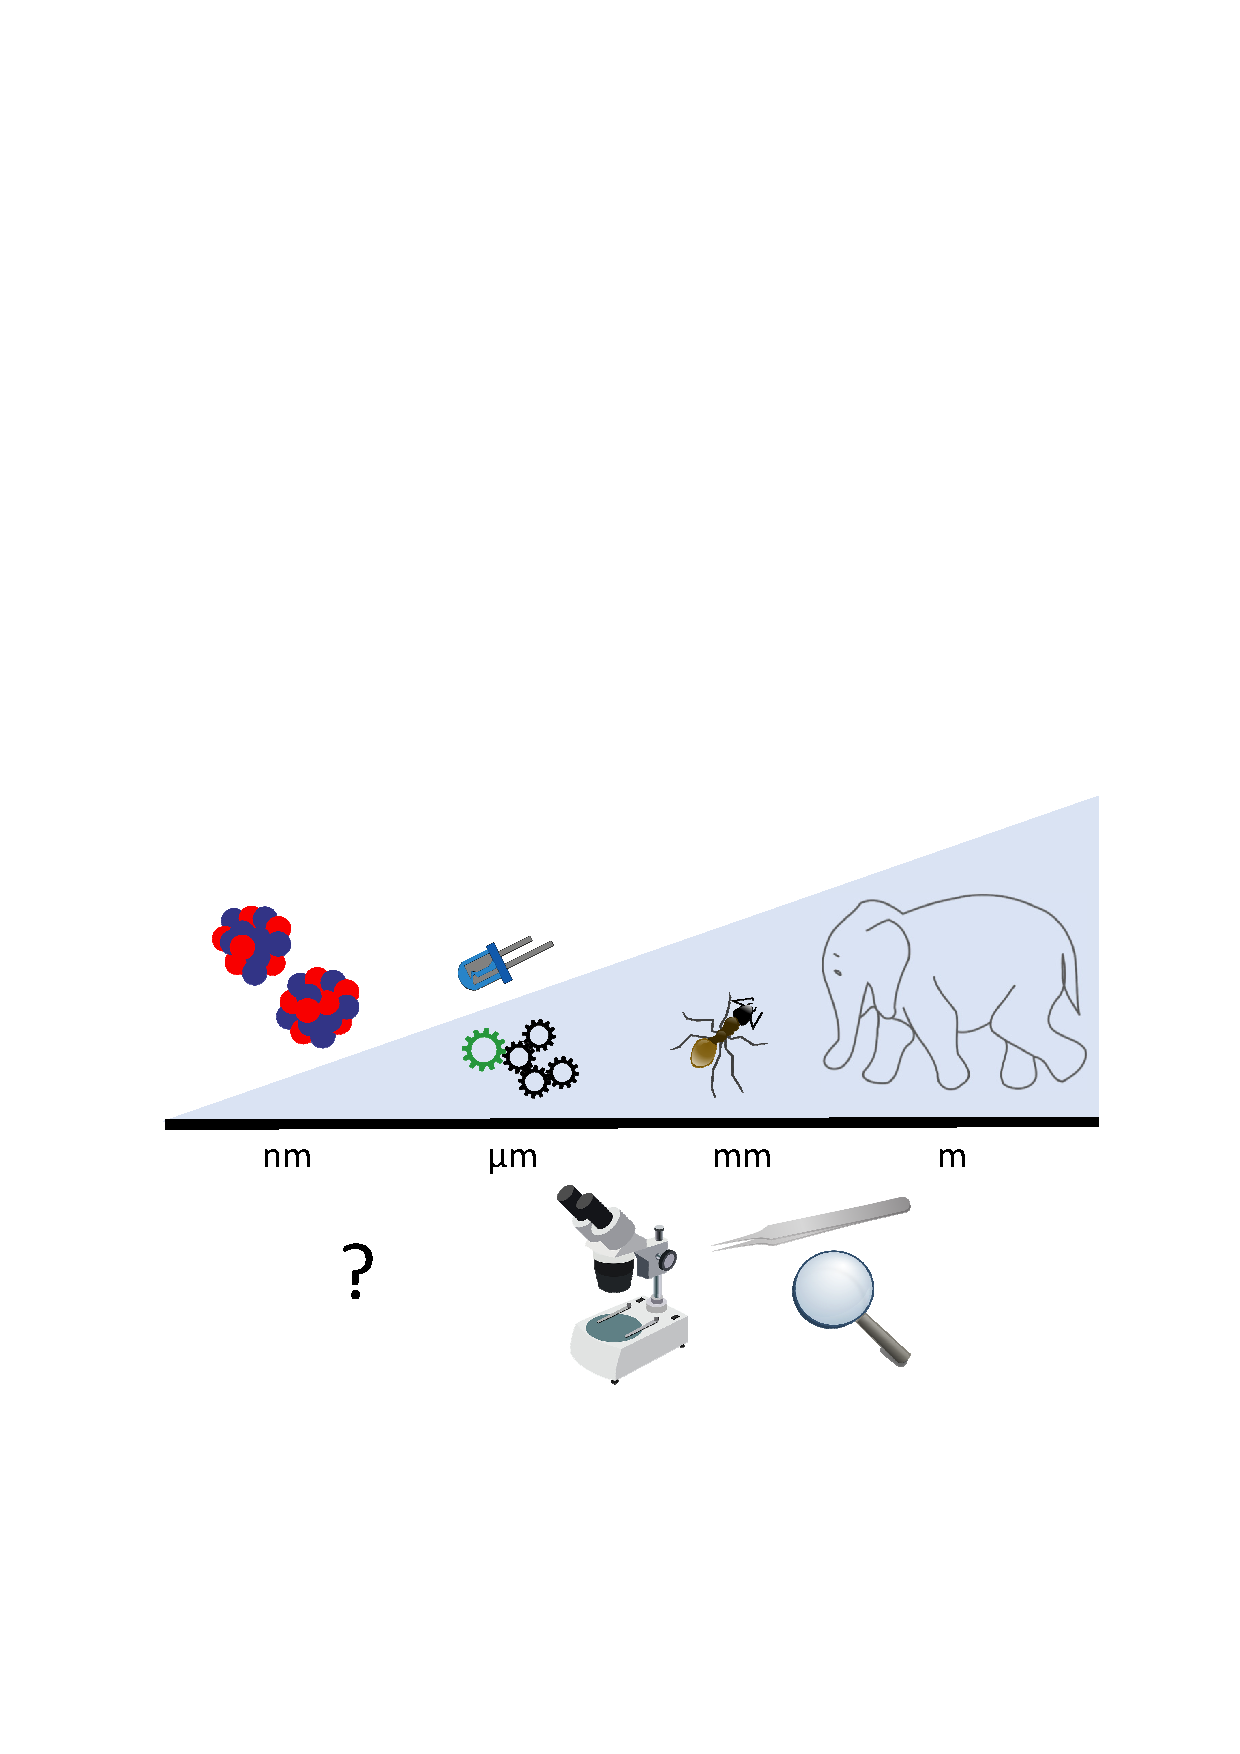
\includegraphics[width=\textwidth]{figures/figure1_scale_problem.pdf}
\caption[Scale problem]{How human beings gain access to lower scales, to see and to manipulate.\footnotemark[1]
\label{fig:1_scale}}
\end{figure}

However, it is not straightforward to access the properties of these nanomaterials and prepare them for real applications. Unfortunately this is due to the above-mentioned issue - small scale. We understand that the observation, reach and built of an object which is $10^6$ to $10^9$ (in one dimension) smaller then any real world macro-object, for example the {\em Great Wall of China} ($21,196 km$), is challenging. Similarly, as compared with human beings' hands, of a size is about $20 cm$, nanoscaled objects are usually million times smaller. Hence, even the nanoscale building blocks are superior in many respects in theory, we are not able to utilize them easily. As shown in Figure \ref{fig:1_scale} \footnote{Without specification, all clip art materials (elephant, ant, microscope, tweezers, etc.) in figures of the dissertation are adapted from Internet which are {\em free to use without permission}.}, we are able to reach smaller scales using tweezers and optical microscopes, but it is very challenging to reach nanoscale objects. 

%introduce to microscopy and probing tech. 
The way human beings make use of fire, tools,  light and electrons is perhaps what sets our modern live standards above of other species. By understanding and utilizing photons, electrons and atomic forces, microscopy allows us to view sub-millimeter objects that cannot be observed with a naked eye. Thanks to the advancement of tools - microscopy and piezoelectric materials - we can now access to nanomaterials by high precision probing technique under direct high-resolution observations. By applying electrical field to a piece of piezoelectric material, the latter precisely changes its shape in function of the applied electric field. Therefore, we may control the mechanical movements by electrical biases and confirm the location of an object and the probe using microscopy. 

\begin{figure}  
\centering
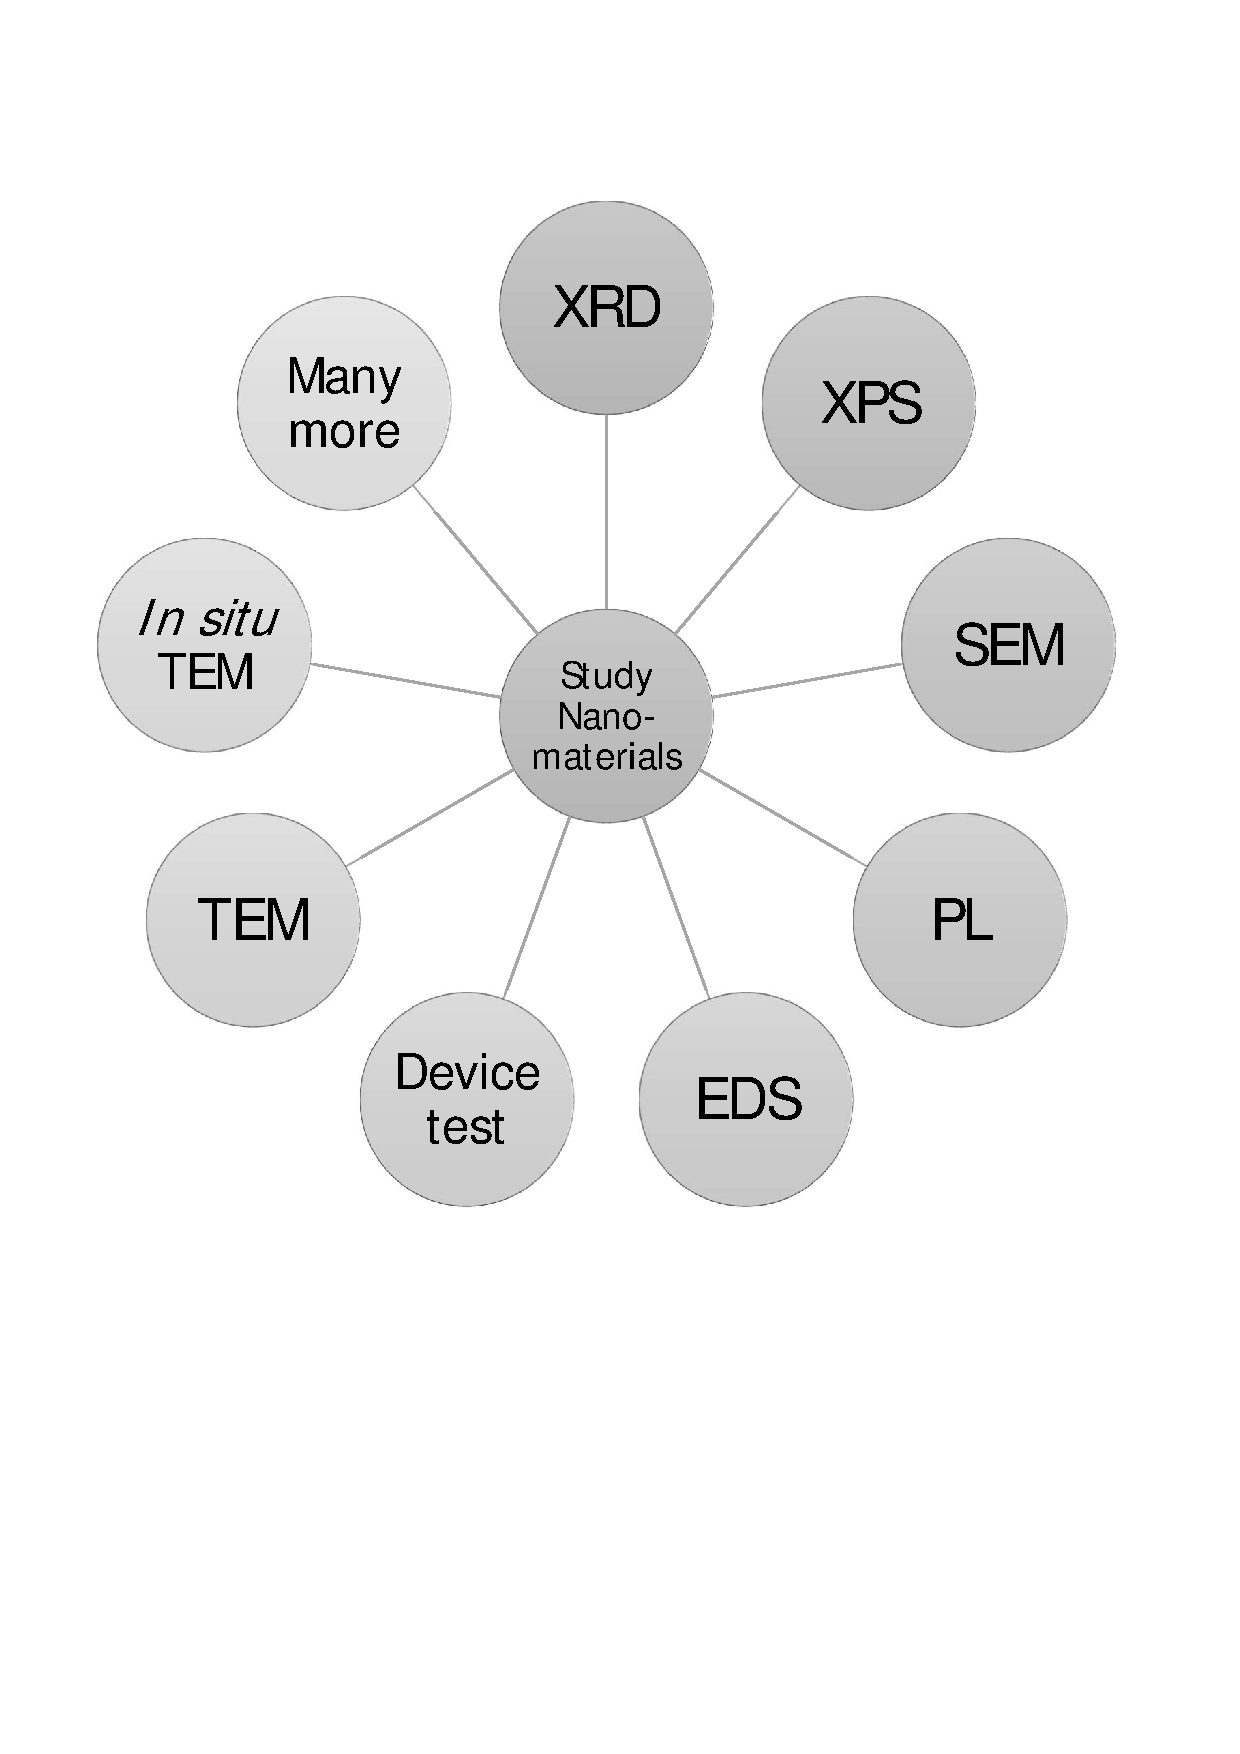
\includegraphics[width=320pt]{figures/figure1_to_study_nanomater.pdf}
\caption[Study of nanomaterials]{{\em In situ} TEM serves as a way to study nanomaterials.
\label{fig:1tsn}}
\end{figure}
%what is in situ TEM

\section{Seeing is believing: Transmission Electron Microscopy}
In the past century, development of particle physics made a way for new microscopies, such as Scanning Probe Microscopy (SPM, including Atomic Force Microscopy and Scanning Tunneling Microscopy), Scanning Electron Microscopy (SEM), and Transmission Electron Microscopy (TEM). Among all microscopies TEM, has the best ultimate spatial resolution; this allows one to reach atomic resolution and to simultaneously get full crystallography information. TEM provides deep and direct information from a thin sample through the transmission and diffraction of electrons. 

When researchers are not satisfied with only seeing of a material in statics, dynamics may be introduced to the sample. \emph{In situ} TEM is the newest advanced technique which gives access to the sample dynamics via observation, manipulation and various tests.\\
Particularly, by adapting the microscope or using a special specimen holder, it is possible to make deliberate attempts to modify materials during high-resolution characterizations. It allows for the observation of dynamic properties of a material under special circumstances.\cite{banhart2008situ}\\

\begin{figure}  
\centering
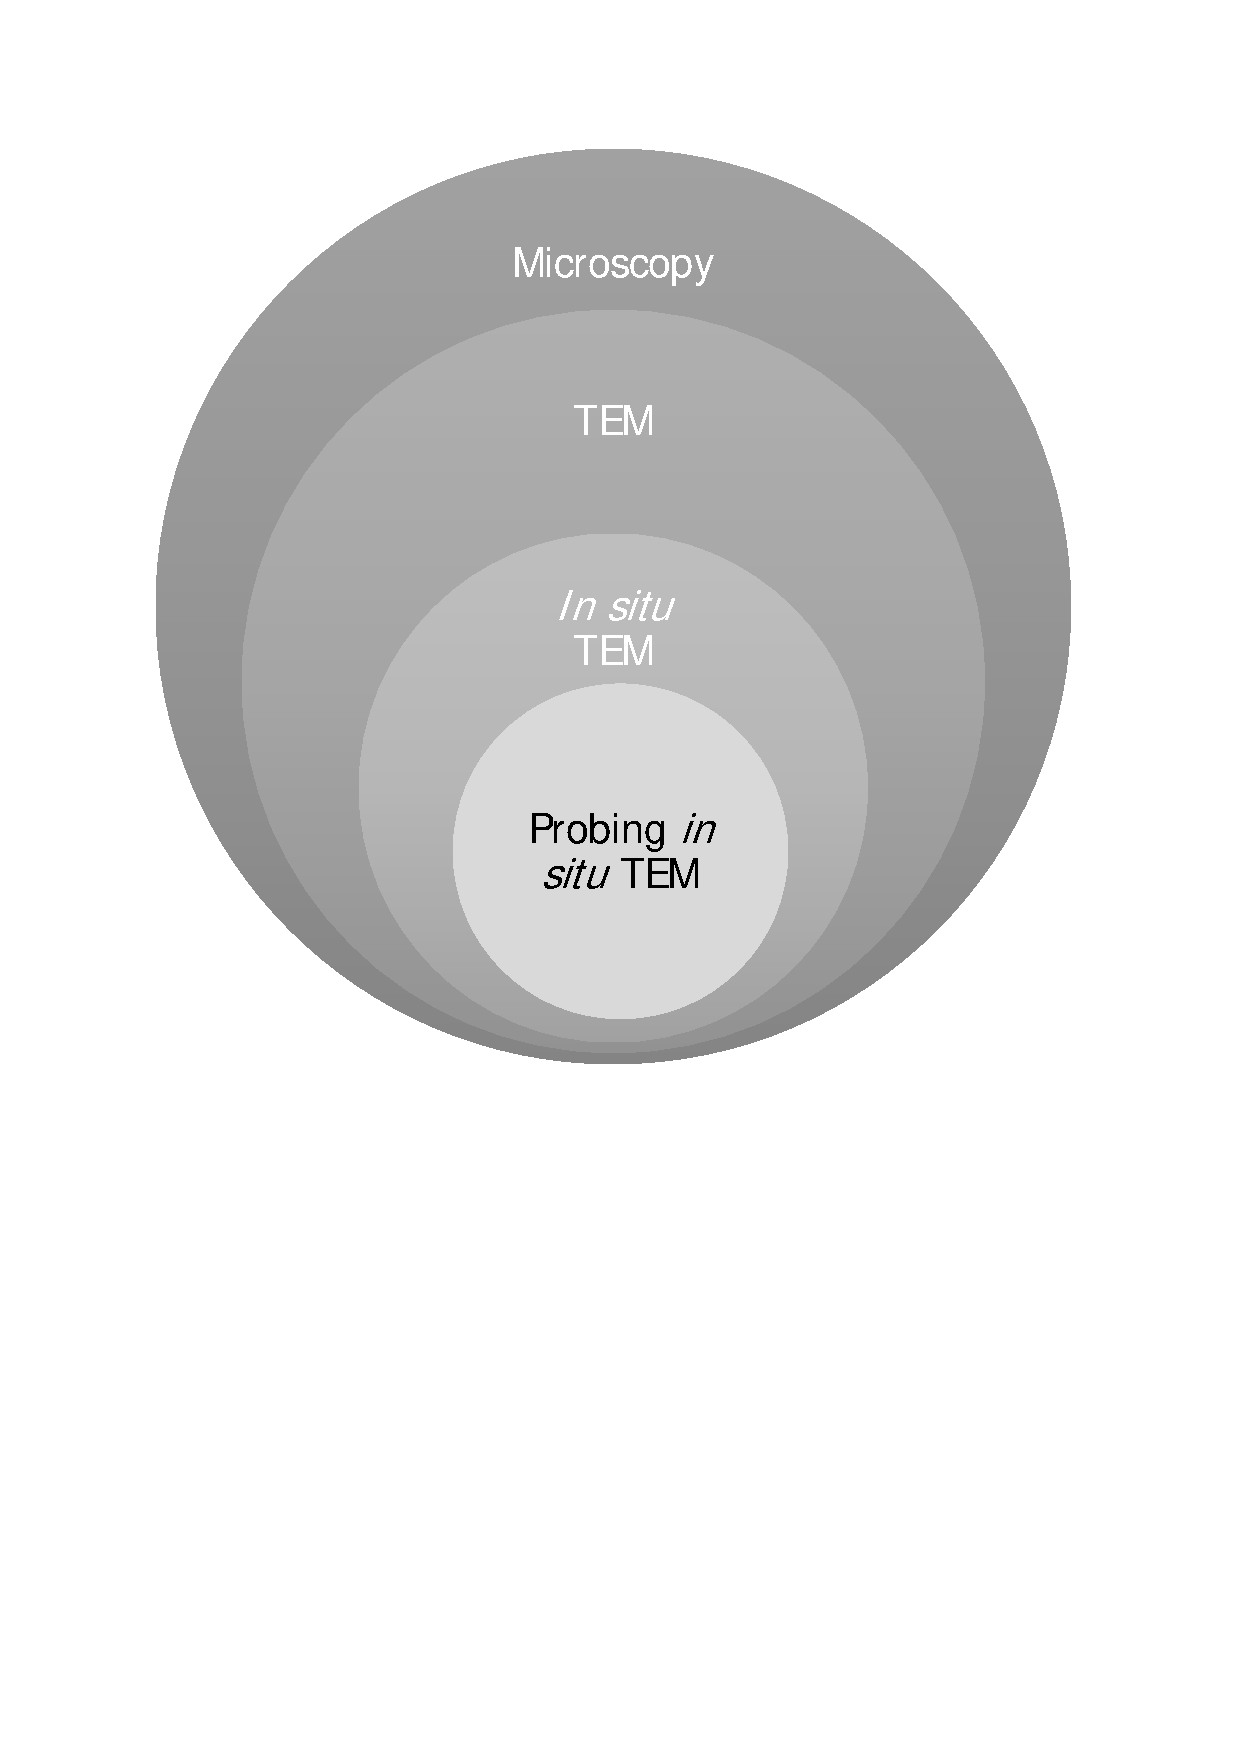
\includegraphics[width=300pt]{figures/figure1_TEM_As_Microscopy.pdf}
\caption[\emph{In situ} TEM as a microscopy branch]{Relationships between probing \emph{in situ} TEM and other microscopies.
\label{fig:1tam}}
\end{figure}

For instance, a heating holder would provide the desired high temperature to trace (by a fast CCD video camera) and thereby reveal chemical transformations within a sample. By contrast, without \emph{in situ} heating, one is  only able to see the initial and final states of the reaction; in this way the regarded mechanism is usually inferred based on a few indirect clues, such as X-ray Diffraction (XRD), X-ray photoelectron spectroscopy (XPS), Energy Dispersive X-ray Spectrometry (EDS), Photoluminescence (PL) and indirect TEM characterizations before and after the dynamic tests. As illustrated in Figure \ref{fig:1tsn}, \emph{in situ} TEM is very important and irreplaceable approach to study nanomaterials. \\

Various specimen holders make it possible to introduce heating, cooling, electrical bias, mechanical force, gas, liquid, magnetic field, light etc. to the sample under various conditions. As illustrated in Figure \ref{fig:1tam}, probing \emph{in situ} TEM is one small domain of microscopy as a whole. This Dissertation is mainly focused on probing of nanomaterials via \emph{in situ} TEM. 

%probing in situ TEM
\section{Untouchable scale: Probing techniques for nanomaterials}

Experiments performed by \textit{in situ} probing microscopy are carried out based on piezoelectric effect and microscopy. \\

\begin{figure}  
\centering
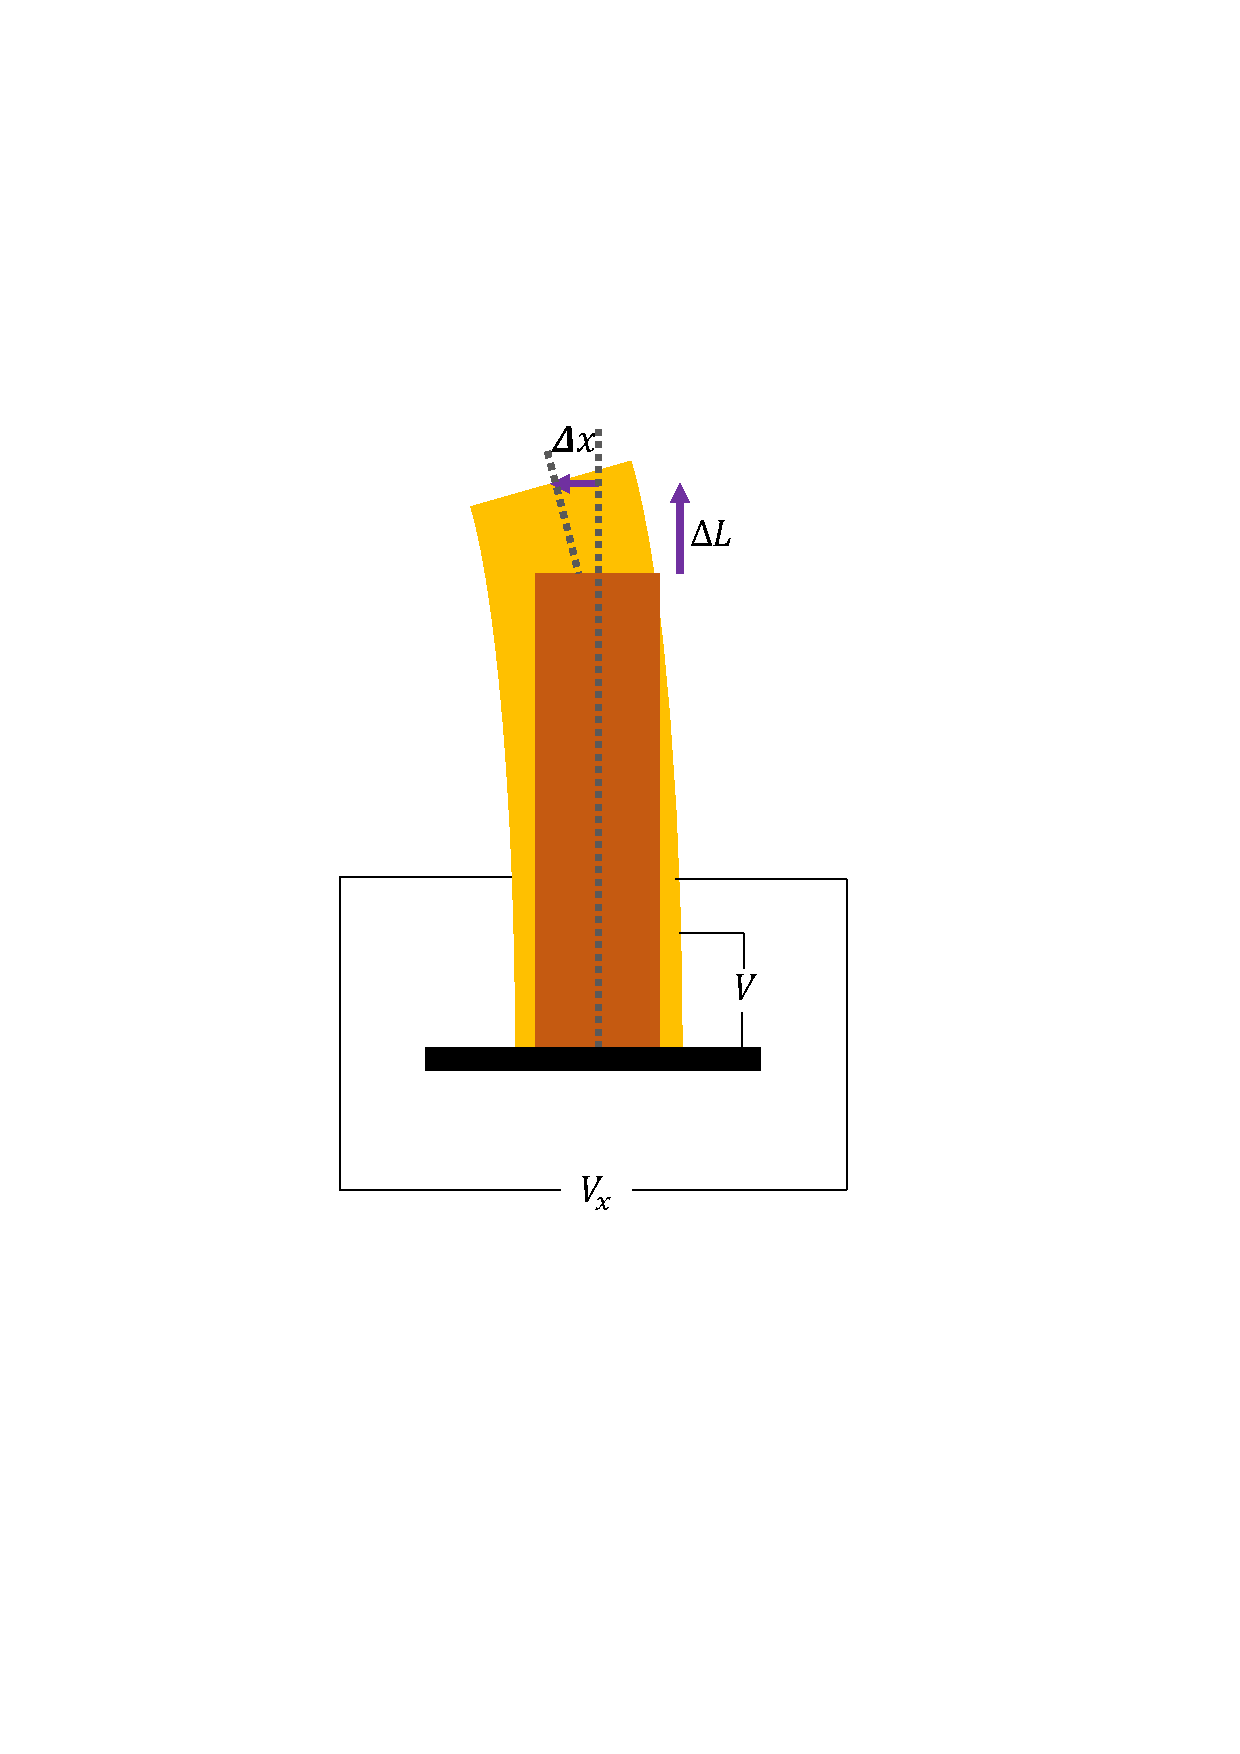
\includegraphics[width=250pt]{figures/figure1_piezo.pdf}
\caption[Probing by piezoelectronics]{Schematic illustration of how piezoelectric works for precised nanomanipulations.
\label{fig:1piezo}}
\end{figure}

Piezoelectricity is a phenomenon where electricity is directly related to the pressure applied to the material. In a piezoelectric actuator, special driving signals are applied to a piezoelectric tube in certain directions, and thereby the piezoelectric tube would respond while changing shape accordingly.\cite{okada2004piezoelectric,vishnevsky1977piezoelectric} As shown in Figure \ref{fig:1piezo}, when the base of the tube is fixed, transverse and axial movements of the tube tip would be expressed approximately by the following equations:
$$\begin{bmatrix}\Delta x\\ \Delta y\end{bmatrix}= \frac{2\sqrt{2}d_{31}}{\pi Dh}L^2\begin{bmatrix}U_{+x}-U_{-x}\\U_{+y}-U_{-y} \end{bmatrix},$$
$$\Delta L= \frac{d_{31}L}{h}V$$
, where $\Delta x$, $\Delta y$ and $\Delta L$ are deflection in $x$, $y$ and axial direction. $U_{+x}-U_{-x}$, $U_{+y}-U_{-y}$ are driving voltages applied to the opposite sides of the tube (therefore in total four electrodes, in addition to the base ground electrode).$V$ is voltage applied to all four quadrants. $L$, $D$ and $h$ is the length, diameter and thickness of the tube. The transverse piezoelectric coefficient $d_{31}$  is very small (about $-10^{-10} \mathrm{m/V}$), and, hence, the movement can be controlled precisely by biasing. 

With a help of a piezoelectric actuator, we can handle an ultrasharp probe to touch the nanoscale sample with the nanometer precision. 
\\
Now we have two effective ways to see and touch a nanostructure -- {\em in situ} TEM and piezo-motor-driven probing. 


\section{Optoelectronic and flexible electronic applications of nanomaterials}
%light to replace electrons
We are currently fully enjoying the benefits of well developed microelectronics and nanoelectronics. However, people are trying to improve the speed of information transmission by means of light. As compared with electrons in the metal (copper or even gold) conductors, photons in the optical system possess much higher capacity of information. The society benefits a lot from the optical fiber information technology. For instance, it was quite difficult and expensive to perform high-definition video streaming \textit{via} Internet 20 years ago when we were using copper wires to transmit electrical information. 
%silicon is not best for optoelectronics
The silicon-based electronics is efficient and is mainly based on the two materials: silicon and copper (or other conductors such as gold). The manufacturing is sophisticated and requires etching silicon chips and applying a mask for electrode coating. Silicon is absolutely perfect semiconducting material. By doping techniques and smart designs, billions of transistors could work at a high speed within a nail-sized chip. The problem is (for optoelectronic applications) that the band-gap diversity is required. Therefore silicon, as a perfect semiconductor for electronics, could not realize fully functioning optoelectronics. \\ 
%silicon is not best for flexible electronics
Besides, flexible electronics attracts a great deal of attention. In the last few years, we experienced an explosion of flexible optoelectronic applications in flat-panel displays, lighting, sensing, and energy cells. For instance, organic light-emitting diodes (OLED) and flexible lithium-ion batteries are developed as a next-generation technology for wearable electronics, bendable smart-phones, foldable displays, etc. However, to make silicon wafers flexible is never an easy task. Therefore, people believe that the bottom-up technology would be able to architect nanoscale building blocks on a flexible substrate for future flexible electronics and optoelectroncs. \\

\begin{figure}  
\centering
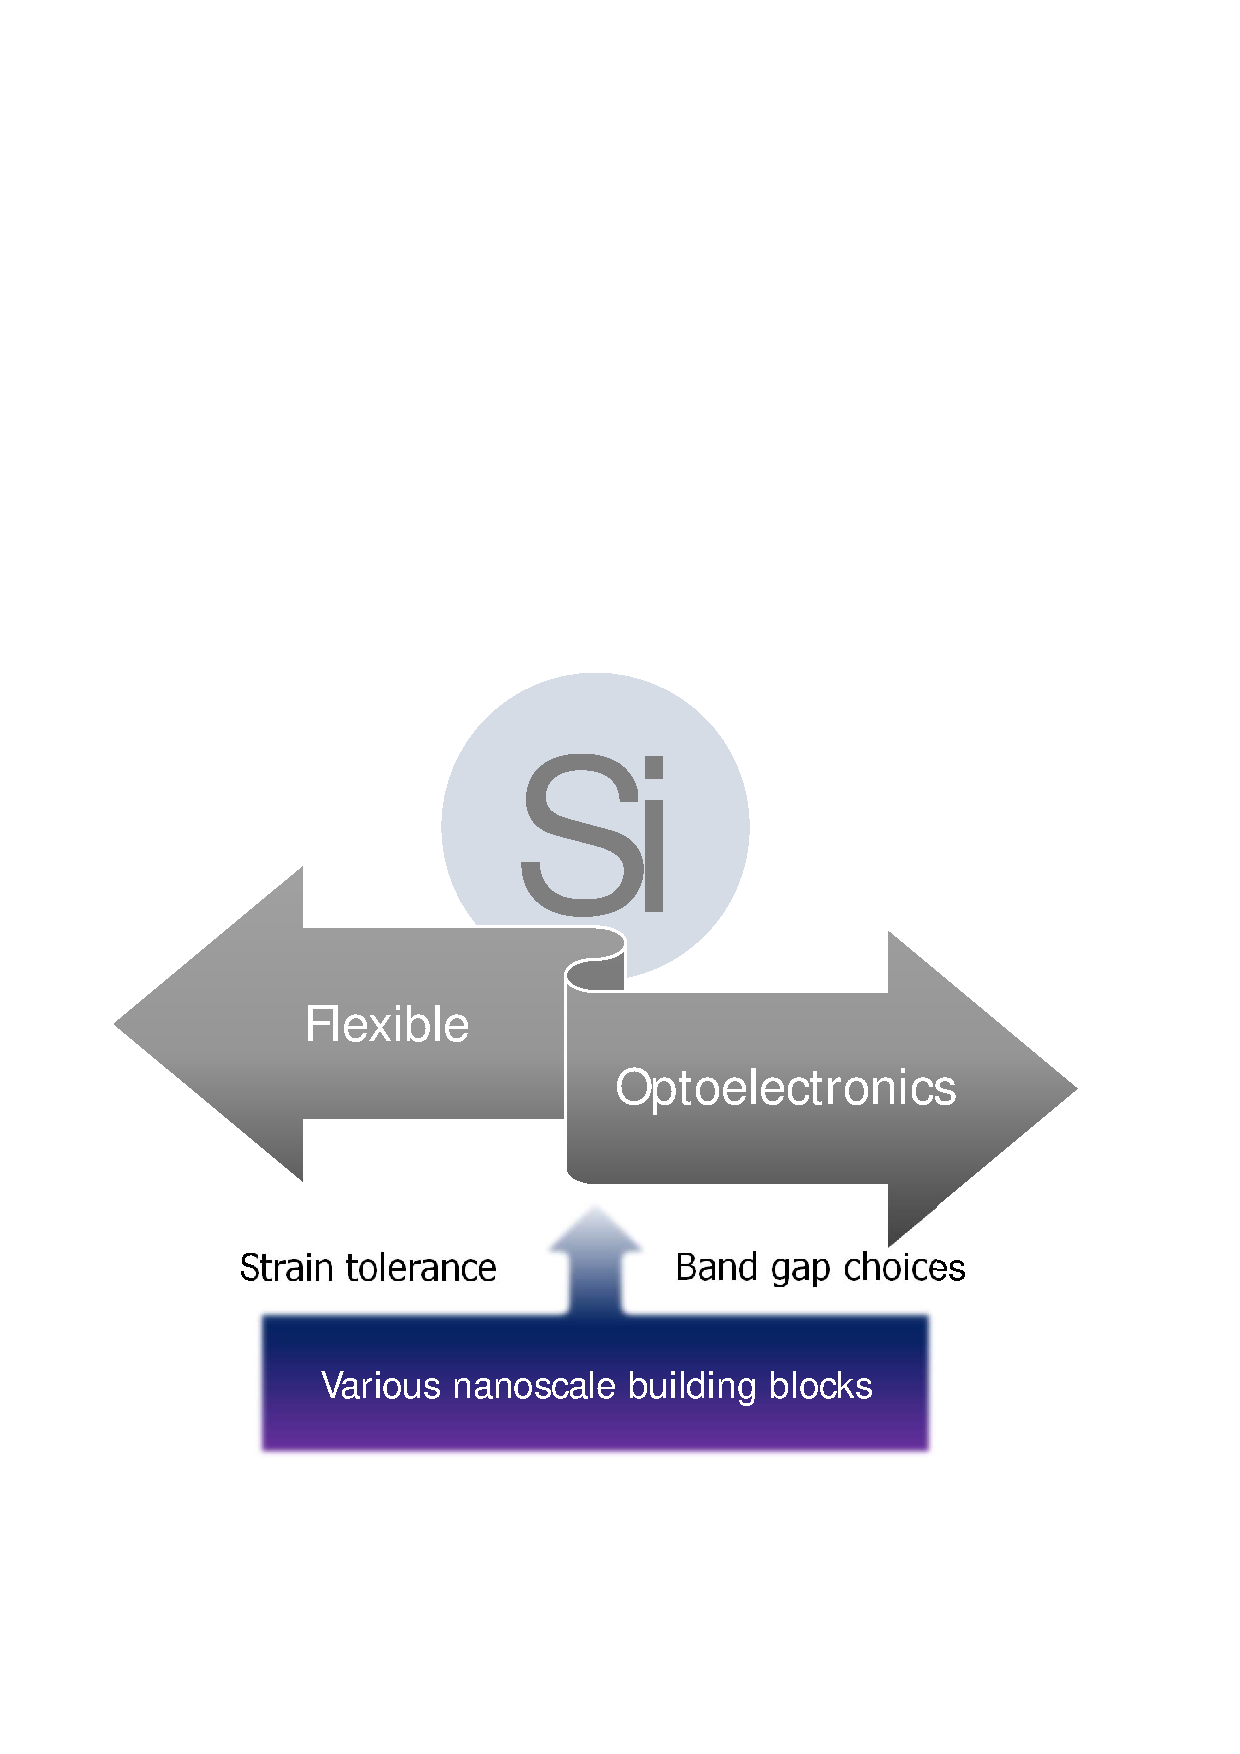
\includegraphics[width=340pt]{figures/figure1_silicon.pdf}
\caption[Future of optoelectronics and flexible electronics]{Silicon's two short-comings for flexible devices and optoelectronics could be backed-up by bottom-up approach using nanomaterials in future integrations.
\label{fig:1si}}
\end{figure}

%So nanomater is good for optoelectronics and flexible applications
Therefore, for optoelectronic and flexible electronic applications, the usage of conventional silicon industries is challenging, as shown in Figure \ref{fig:1si}. Silicon  is an ideal material to meet all requirements within a field effect transistor. The silicon based devices rely on controlling carriers realized \textit{via} structural design and doping. In recent years, silicon-based optoelectronics is growing steadily but not exponentially, as expected by Moore's Law. \cite{Waldrop2016} 
The semiconductor industries produce devices mainly by the top-down strategy. A top-down approach is a smart way to apply desired patterns to the device engineering, which came in effect since 1970s, when human beings were not so experienced to manipulate nanostructures. However, these days a bottom-up approach is emerging and shows a high promise in constructing systems by piecing building blocks together. It is true that some nanomaterials show superior properties for electronics, but it appears that during the last decade, many efforts from various research groups have been unable to establish bottom-up technology as a real market value. \\
It is expected that in the future high quality nanomaterial building blocks could be well handled for device integrating by the automated mass production. The integrated LDs, LEDs and photodetectors could be manufactured using nanowires, nanosheets and even quantum dots to realize fully functioning optoelectronic chips. The current obstacle is to get more knowledge of the building block materials. How does the electrical signal from nanowires or nanosheets behaves under strain and light illumination, what is the photocurrent spectroscopy of the material - such questions are not well studied. Consequently, it is strongly required that we find the answers to these questions in order to provide clues for future flexible electronics and optoelectronics. 

\section{Energy storage applications of nanomaterials}
%energy is important
Electrical energy storage will be far more important nowadays than it was when we had abundant petroleum resources, and when we didn't have smart (smart also means energy consuming) electronics. From powering portable electrical devices (cell phones, tablets, laptops), implantable medical applications (pacemaker), to machines (hybrid electric vehicles), the humans' desire for clean, safe, fast and efficient energy storage is becoming more and more  significant. \\
%ion-batter is important
Among all energy storage applications, lithium ion-batteries (LIBs) are the most needed devices due to their high energy density, which is the key factor for portable electronics and automobiles. In LIBs, lithium ions move from the anode to cathode during discharge, and from cathode to anode during charging. The materials for the anodes and cathodes can dramatically affect the few key aspects of the battery’s performance, including stability and capacity. High capacity materials are eagerly demanded in order to address the needs for better energy density, cycle life and charge lifespan, among other issues faced by Li-ion batteries. 
%Nanomater for ion-battery
However, conventional materials, although being  well developed,  still cannot catch up with the growing demands of battery capacity. Li-ion batteries have struggled with numerous issues, such as poor cycle life, rising internal resistance with cycling and aging, safety concerns (especially when overheated or charging problem), and growing applications demanding higher capacity. \\
A lot of researches have confirmed that nanomaterials are particularly promising to solve these problems. The advantages are as follows\cite{Bruce2008,qifengzhang2013csr}: \\
\begin{itemize}
	\item[a] Many nanomaterials enable electrode reactions to become reversible while they are not reversible for bulk materials; 
	\item[b] The reduced size significantly increases the rate of energy transformation between electricity to chemical energy (such as lithiation and delithiation process) due to the short diffusion lengths; 
	\item[c] Electron conductivity can also be improved in nanomaterials; 
	\item[d] High surface to volume ratio provides high contact area between electrodes and electrolyte; 
	\item[e] Chemical potentials of ions and electrons can be different at the nanometer scale, and, therefore, electrode potential can be modified. 
\end{itemize}

\begin{figure}  
\centering
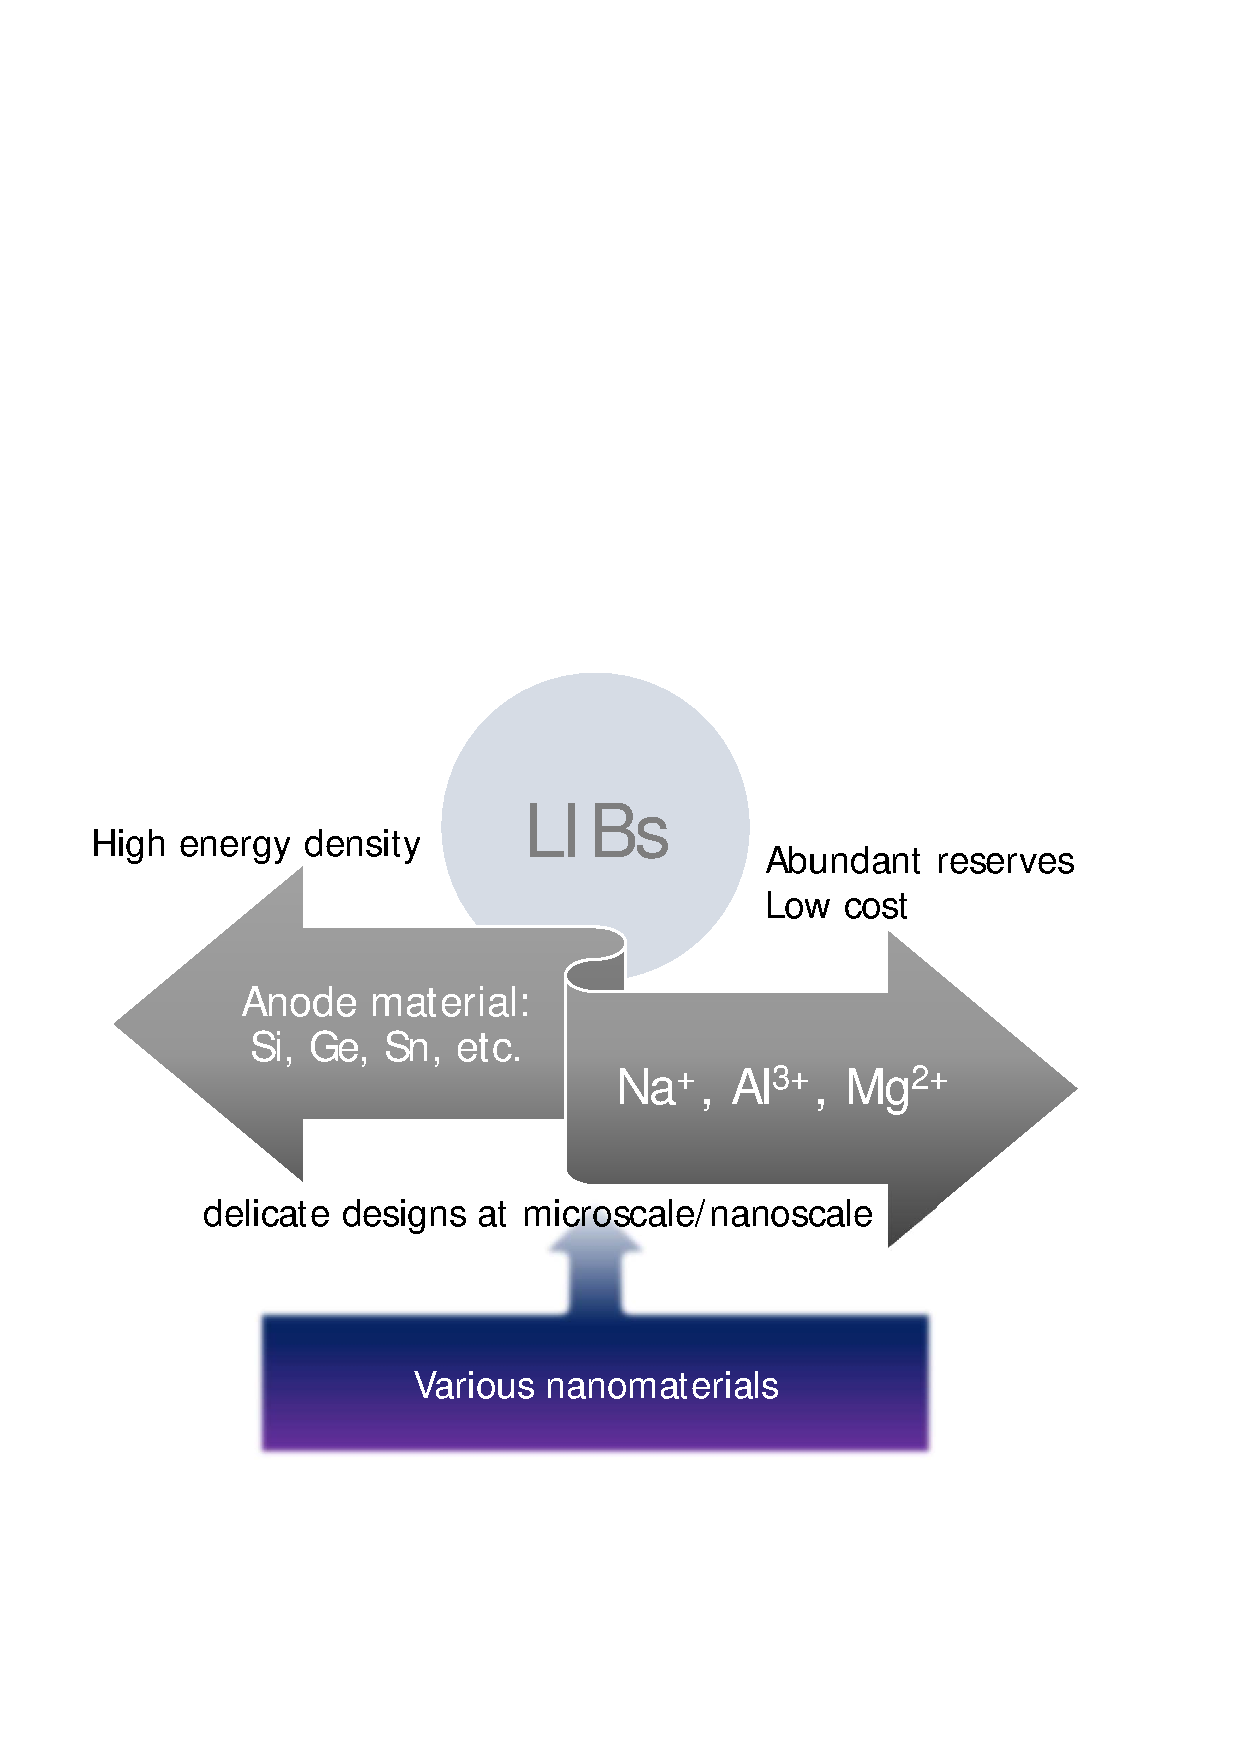
\includegraphics[width=340pt]{figures/figure1_lib.pdf}
\caption[Future of secondary ion batteries]{\textcolor{red}{A scheme showing that secondary batteries are mostly based on Lithium and graphite. However, to gain a higher energy density while using cheaper/abundant elements, nanomaterials might be the key. }
\label{fig:1lib}}
\end{figure}

%silicon for ion battery anode
 Graphite has widely been used as an anode of choice for commercial products, since the first generation of Li-ion chemistry studies appears. Due to strong needs of high capacity, in recent years, researchers have been interested in developing silicon anode materials for high capacity lithium-ion batteries. Among all investigated anode materials, silicon has one of the best  theoretical capacities of $3590 \mathrm{mAh/g}$ (about 10 times higher than carbon) based on the fully alloyed form of \ce{Li15Si4} at room temperature (at high temperature \ce{Li15Si4} can be obtained, giving a capacity of $4200 \mathrm{mAh g−1}$, placing it on top of all other anode materials. In addition, Si anodes show moderate working potential at $0.5$ V, which is higher than graphite anodes at $0.05 $ V. This means that silicon is suitable to solve the safety problem of lithium deposition upon cell overcharge as well as avert the energy penalty of battery cells assembled with the \ce{Li4Ti5O12} anodes.\\
 However, the insertion/extraction of lithium ions result in significant volume change - about 370\% - which leads to structural pulverization and electrical disconnection between anode materials and current collector, and finally the battery loses most of its functions. Some recent designs of LIBs using silicon materials as anodes allows the battery to maintain its initial anode structure and hence to reach high capacity while, at the same time, good stability. 

 Cui et al. designed high performance anode structure using Si nanowires, which were able to accommodate large strain caused by lithium ion insertion and extraction.\cite{Cui2009} 
 Deng et al. reported a tubular configuration made from rolled-up C/Si/C layered nanomembranes which performs with a highly reversible capacity at approximately 2000 mAh /g (50 mA/g), and has approximately 100\% capacity retention (500 mA/g) after 300 cycles.\cite{Deng2013}
 Cui et al. also designed core-shell structures for Si-based LIBs. They proposed a hierarchically structured Si anode which was inspired by the structure of a pomegranate. Si nanoparticles became encapsulated by conductive carbon coatings. This leaves just enough space for the expansion and contraction during lithiation and delithiation cycles. \cite{Liu2014d}
   
\begin{figure}  
\centering
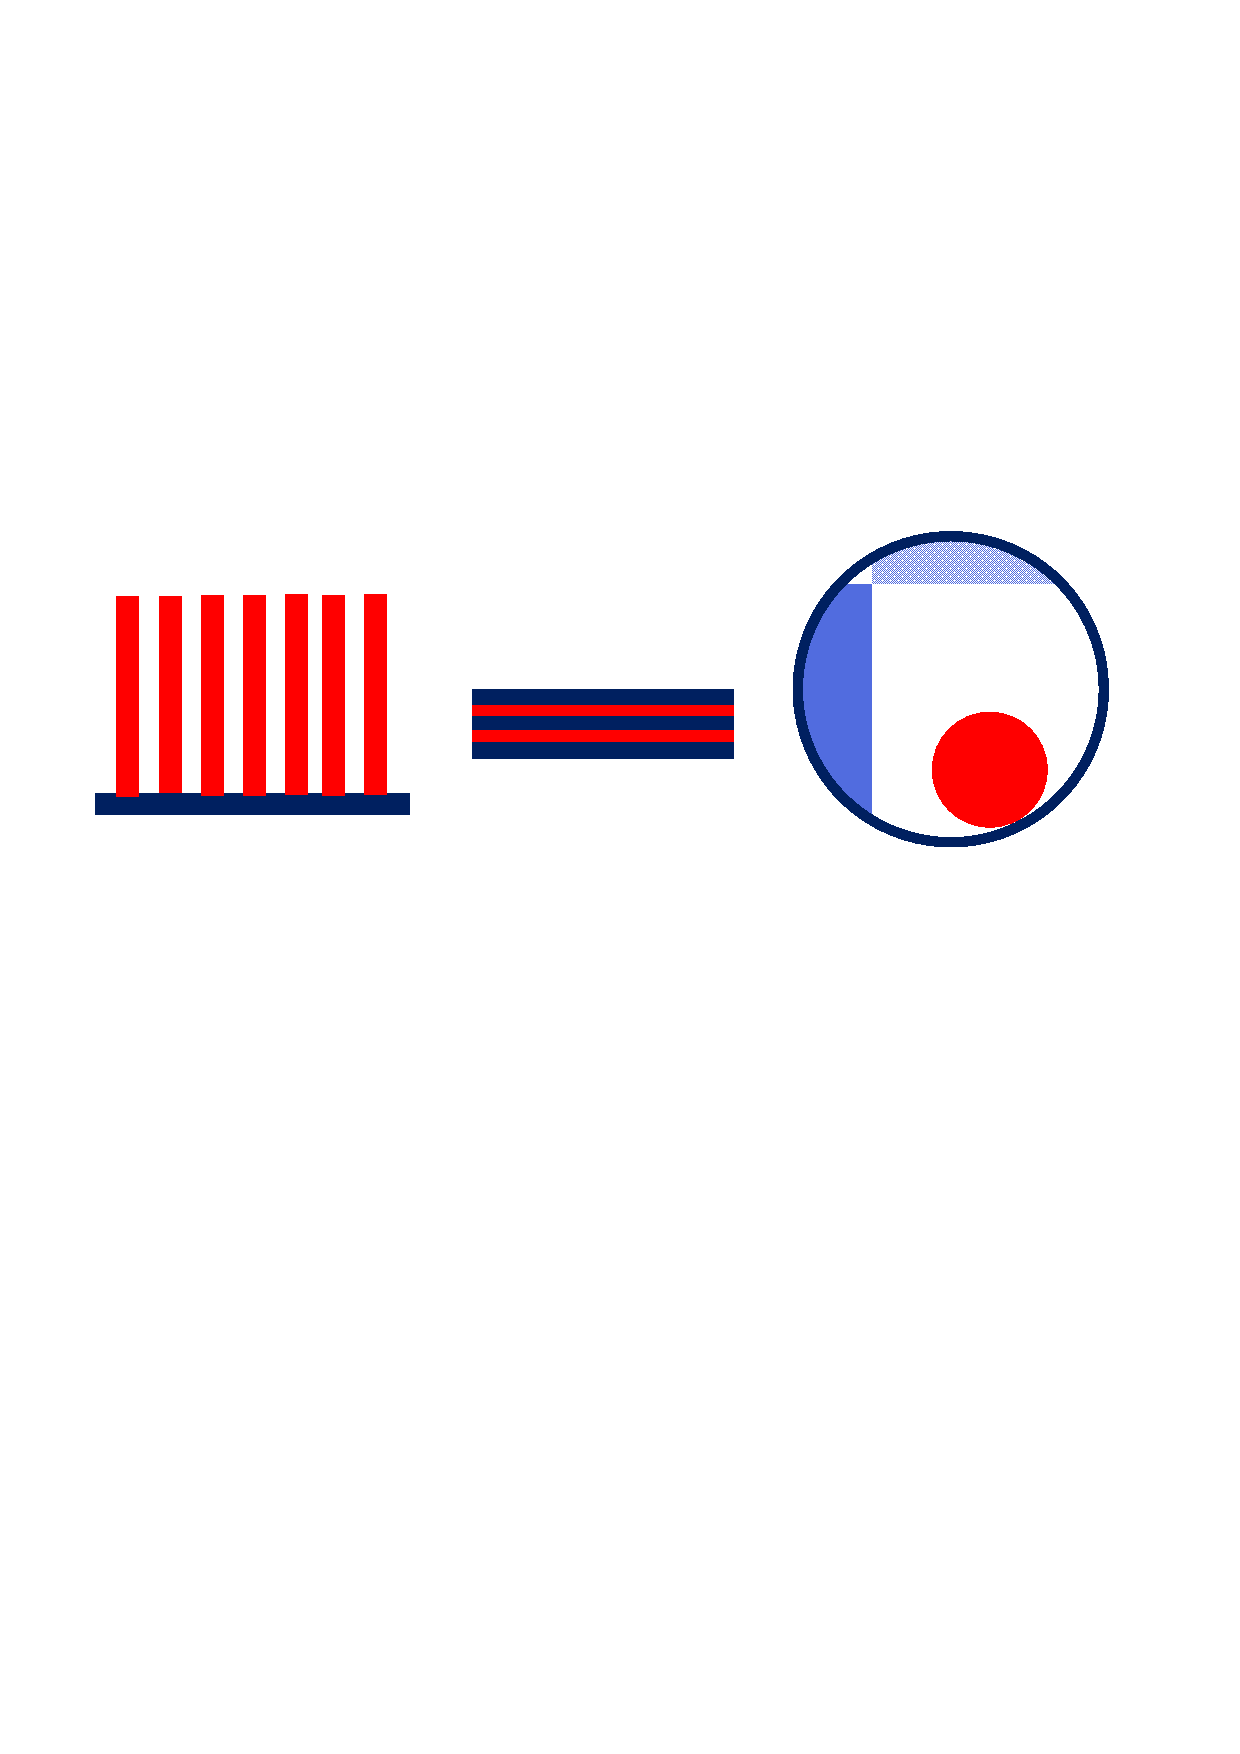
\includegraphics[width=\textwidth]{figures/figure1_silibdesign}
\caption[Designs for large volume expansion anode materials]{Designs for large volume expansion anode materials in batteries. Red correspond to material with large volume expansion/shrinking during cycling, while material in blue color is the confinement material with low volume expansion rate and good mechanical strength. 
\label{fig:1silibdesign}}
\end{figure}
 
Therefore, by designing the microscopic structures, one is able to utilize the high capacity material under structural and mechanical restrictions, as illustrated in Figure \ref{fig:1silibdesign}. Also, many other attempts of combining silicon with carbon materials,  polymers,  metals, were summarized by Liang et al.\cite{Liang2014} 
 
%Na-ion batteries
It is predicted that lithium would be the next energy resource which substitutes for petroleum, which will die out.\cite{Jaskula2016} According to the distribution of lithium on Earth\cite{Jaskula2011a}, Chile could be the next Saudi Arabia it terms of richness of resources. This problem is more essential for many countries with very limited lithium reserves, such as Japan. \\
In order to explore the next generation of secondary batteries, which are called post-lithium ion secondary batteries, many investigations
show that the most promising candidate is the sodium-ion battery (SIB). SIBs use sodium instead of lithium as the charge carrier, and use iron, manganese and other transition metals to replace cobalt for redox reactions. SIBs are expected to be mass produced in the nearest future due to their minor environmental impacts and low cost.

\begin{table}[ht]
\centering % used for centering table
\begin{tabular}{|l|c|c|} % left, centered columns (3 columns)
\hline %inserts double horizontal lines
 & LIB & SIB\\ [0.5ex] % inserts table heading
\hline % inserts single horizontal line
Theoretical capacity & 3,829 mAh/g & 1,165 mAh/g \\[1.5ex] % inserting body of the table
Cost (carbonate) & 5,000 USD/t & 150 USD/t \\[1.5ex]% [1.5ex] adds vertical space
Reserves & 23,000 ppm & 20 ppm \\[1.5ex]
Potential & –3.045 V & –2.714 V \\[1.5ex]
Ionic radii & 79.3 pm & 100.9 pm \\[1.5ex]
\hline %inserts single line
\end{tabular}
\caption{Comparison of LIB with SIB.} % title of Table
\label{table1.1} % is used to refer this table in the text
\end{table}

As shown in Table \ref{table1.1}, although sodium possesses a higher normal electrode potential of ~0.3 V, larger effective radius than lithium (in volume ratio 2.05), and smaller theoretical capacity, the cost and environmental benefits are still very attractive for applications which do not require very high capacity. Actually, it is hard for graphite, which is commercially used as an anode material for LIBs, to store and release sodium ions both theoretically and in practice because of the size of sodium ion is large. \\
However, it was discovered in 2000 that hard carbon having disordered structures could electrochemically store and release sodium ions.\cite{Stevens2000} Several years ago, a work was done on developing and making practical sodium ion batteries, and since recently researchers have been investigating on many anode active materials for sodium ions. It is worth noting that well-established guidelines and experiences acquired for LIBs electrode active materials are not applicable for SIBs.\cite{Lang2010,Armand2008,KUZE2013}

Consequently, the two important research areas of secondary batteries are: finding better anode active materials with higher capacities, and looking for other elements for ion batteries, as illustrated in Figure \ref{fig:1lib}. To apply these elements in secondary batteries, nanomaterials, or nanoscaled designs play very important roles. They enable reactions which may overcome huge volume expansion, to decrease diffusion lengths; while bulk materials are not capable to reach the highest capacity either for LIBs or for special ion-batteries at the moment. 

\section{Motivation of my PhD research}
As stated above, {\em in situ} studies on nanomaterials toward optoelectronics, electronics and ion batteries are required by the Society. My motivation is to take the challenge and to analyze the dynamics of the building blocks, as well as heterostructures, and to provide decent knowledge for advanced applications. 
Therefore, I explored some experimental methods and engineering details, including {\em in situ} TEM setups and the working mechanisms. \\
Then I present manipulation possibilities in the frame of the general \textit{nanoarchitectonics} concept and its applications for nanoengineering. The experiments have been performed on the {\em in situ} TEM-constructed axial nanowire junctions of CdS and p-Si. In addition, detailed electrical probing for energy storage research is discussed. I fabricated an ultra-stable sodium ion battery and analyzed the mechanism of its cycling performance under {\em in situ} TEM probing. Through coupling with {\em in situ} TEM applied mechanical forces, two examples of force-driven optoelectronic phenomena are detailed using the examples of ZnO and CdS. 
%update: Jan 14 fixed grammar according to prof notes
%update: Jan 13 add figure 4ways
%update: Jan 09-11 prof check
%update: finish writing Dec 30
%note: image 4waysprobe is not here

%\begin{savequote}[75mm] 
%We become what we behold. We shape our tools, and thereafter our tools shape us.
%\qauthor{Marshall McLuhan} 
%\end{savequote}

\chapter{Engineering of Probing Techniques inside TEM}

\newthought{We are not satisfied with the limited possibilities provided by TEM}, and we are eager to introduce more variables to the system because that is how we see dynamics in the real applications.
In the following subsections, I will firstly introduce how we cooperate chemicals, light, mechanical manipulations and electrical interactions within a microscopic experiment. 
Especially, for the new optical fiber compatible TEM, where all the four factors could be merged, the inside and outside parts of the \emph{in situ} microscopic setup are described in detail. 
Finally I will take a look at what the system can do and its short-comings. 

\section{Introducing chemicals, electricity, strain into the microsocpe}

As I discussed in Chapter 1, \emph{in situ} microscopy does introduce parameters such as heat, cooling, gas, liquid, etc. to the system, but now I focus on how we delicately introduce these variables into the  microscope. In most cases, {\em in situ} microscopic experiments are performed by means of specially designed TEM holders, such as, heating holder equipped with the heating electrical wire or MEMS microheater. At the same time, some researchers made adaptions to the microscope, to introduce other variables. In my Ph.D. research, in addition to the electron beam, four more variables are introduced: chemicals (solid), mechanical probing, electrical contacting and optical access. \\

For electrical biasing, many TEM specimen holders are commercially available. Such holders provide a combination of TEM and Scanning Tunneling Microscopy(STM) techniques, which are employed simultaneously within one instrument. TEM characterization, STM imaging, introducing chemicals and electrical measurements- all become possible. A STM probe scanner has a very wide range of motions, from picometers to millimeters, which are employed either for a coarse adjustment of the sample orientation, or for the precise probe positioning. \\

Electrical contacts with nanoscaled interfaces can be realized under precise positioning of the movable probe to the desired spot, enabling simultaneous investigation of the specimens' structural and electronic properties under the optional strain or chemical transitions.\\

If the electrical biasing is realized through piezo probing, we can also utilize the probe for introducing chemicals (solid on probe) and a mechanical strain (without force value measurement\footnote{Introducing atomic force microscopy into TEM holder for mechanical measurements is another important {\em in situ} method without electrical biasing functions.}). \\

I briefly discussed the ways to input chemical, electrical biasing and mechanical factors in TEM. However, introducing  the other variable - light - to the system is most challenging. Therefore, I will discuss this part separately, which would be a very good reference for future research, in the next section. 

\section{Introducing light into the microscope}
\subsection{Previously}
Introducing the other factor - light - to the system, while at the same time maintaining the impact from other factors, is very tricky. Some researchers and companies tried to introduce light without probing. This means that no introduction of chemical changes, electricity and mechanics was achieved. We may first investigate how they introduce/collect light to/from the microscope. 
Table \ref{table2.1} compares the two possible ways to implement light into the system. 

\begin{table}[ht]
\centering 
\begin{tabular}{|c|c|} 
\hline 
by adaption to the microscope & by using special holder \\ [0.5ex] 
\hline 
light plane different from specimen & on same plane with specimen \\[1.5ex] 
require take off detector/aperture & a specially designed holder \\[1.5ex]
optics can be realized by lens on bench & only optical fiber\footnote{For the moment only optical fiber, but it is possible to have lens system inside the holder, please read Chapter 7 for more information.} \\[1.5ex]
complicated, high power, high cost & no adaption to TEM\\[1.5ex]
\hline
\end{tabular}
\caption{Two main ways to shine light into a TEM} 
\label{table2.1} 
\end{table}

As shown in the Table, by replacing an aperture or making a window for optical path the light path becomes tilted. The light goes through the microscope body at the different level from the specimen plane. In some cases, it is possible to replace a detector or an aperture by desired modules to provide more variables. As shown in Figure \ref{fig:2_1} under a certain angle, the light can reach the specimen. The system could be very complicated if the optics is realized through the lens system on optical bench including light sources, lens system and options such as CCD camera, chopper and monochromator. The system can be very powerful if the optical system on table is well designed and precisely assembled. However, the pressure of time and high cost are expected to be very significant. \\

\begin{figure}  
\centering
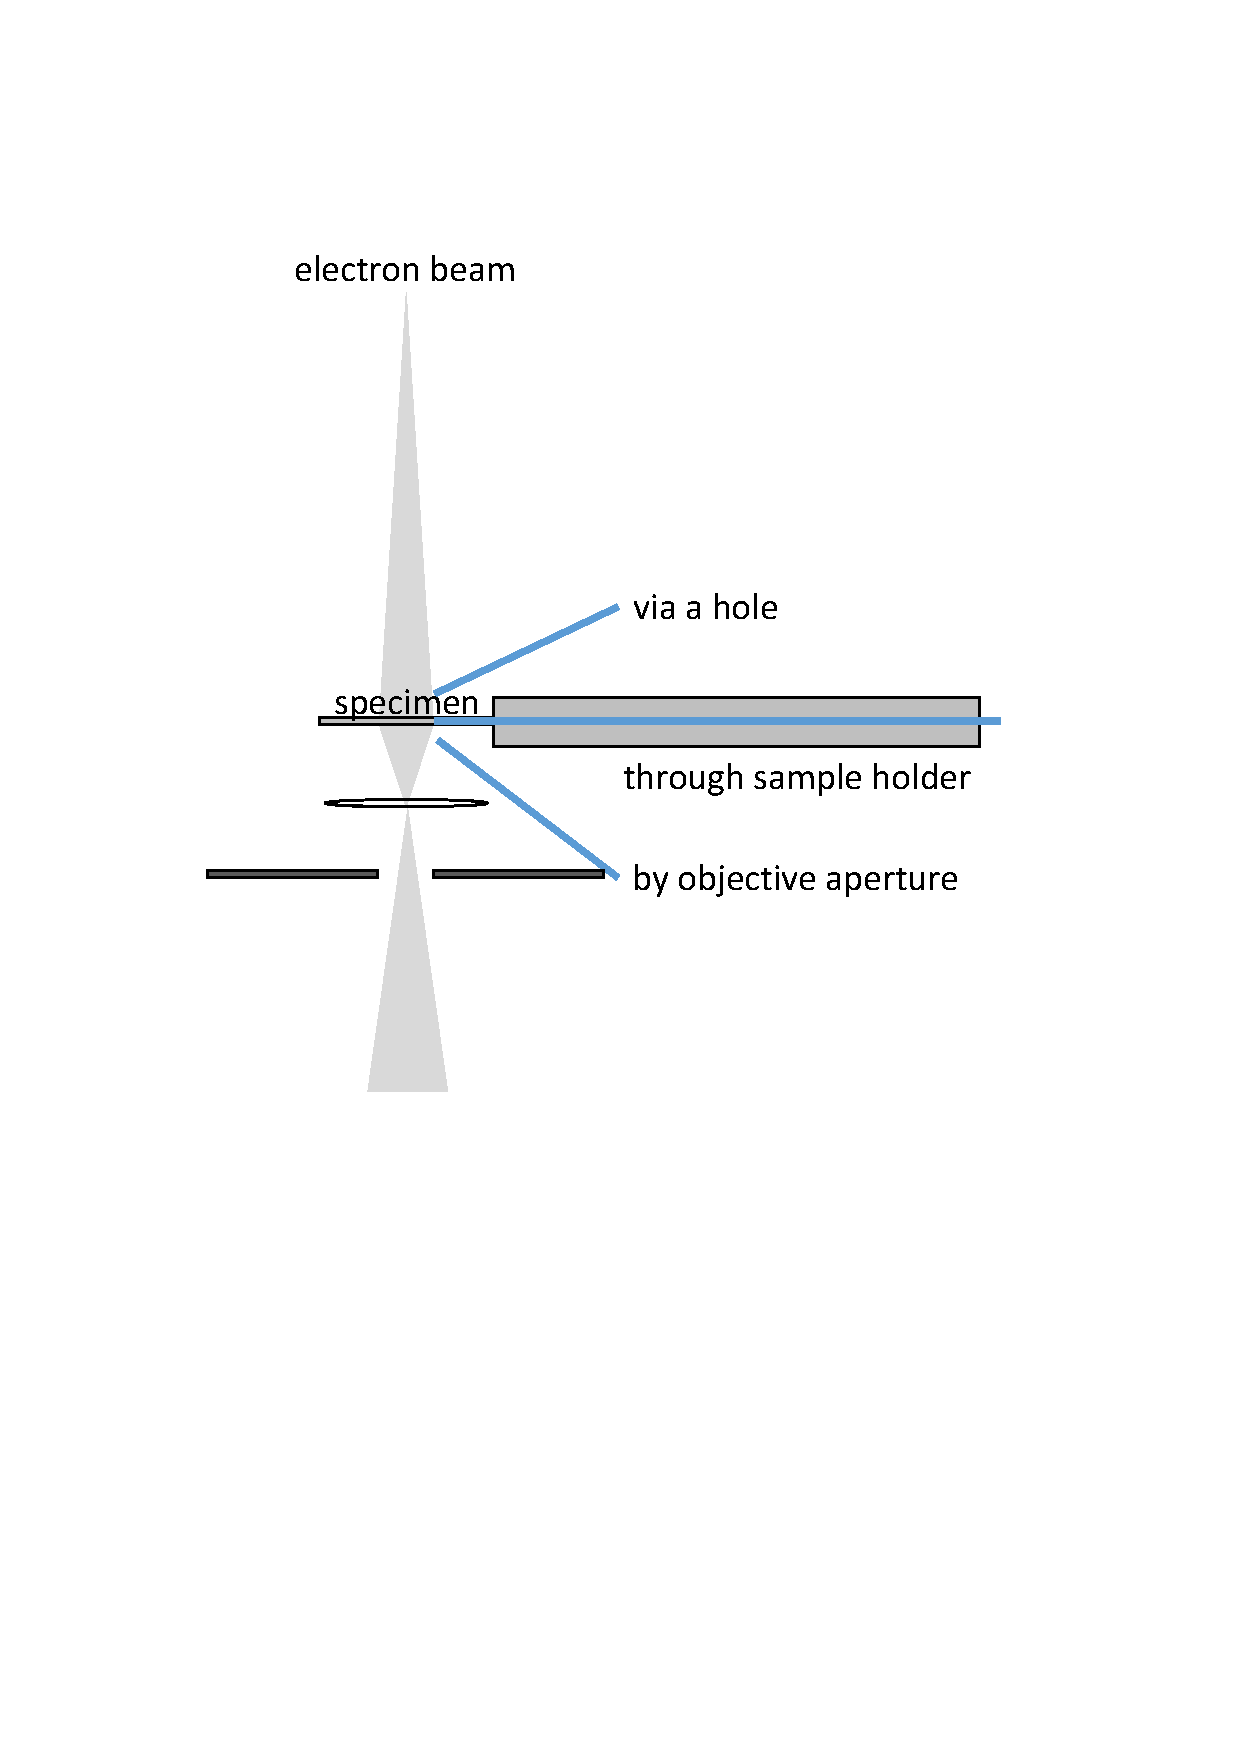
\includegraphics[width=320pt]{figures/figure2_1}
\caption[Putting light into TEM.]{How light is compatible to TEM.
\label{fig:2_1}}
\end{figure}

For a special optical holder, one way is to protrude an optical fiber through the holder, as shown in Figure \ref{fig:2_1}, the light will be shinning on the specimen at about 90 degrees to the direction of the electron beam. In most cases, the microscope is owned by many users for various applications, and, therefore, the approach of using special optical holder is more practical - it's quite unpractical to drill a hole in the microscope column and to install an optical bench on the microscope (given the fact that not every user will be happy with such operations). \\
A few groups have tried to deliver light into TEM. \\
Muto et al. (Kyushu University) managed to install an optical fiber through a 2 mm hole at an angle of 45 degrees.\cite{Tanabe2002,Furumoto2013} They manufactured the prototype of TEM-CL system with the light collecting parts integrated on the holder, but no parabolic reflector was needed within the pole piece. The system is able to take cathodoluminescence(CL), X-ray emission spectroscopy and Electron Energy Loss Spectroscopy (EELS) at the same time, even under large angle sample tilts. The main disadvantage of the holder was a significant background level from the thermal glow of the electron gun and the CL signal from the optical fiber. Later, the same group and the staff from {\it Nanofactory Instruments} developed a prototype optical holder implemented with an optical fiber inserted through the holder, on the side of a specimen. The reflectors and optical fiber are placed away from the TEM optical axis. The light-collecting solid angle is approximately 1.3 strad, approximately 100 times larger than that of their first generation prototype. The sample is mounted at the end of the metal wire, which  position can be controlled to the focal point of the mirror by a piezo-driven manipulator. In years of 2012-2013, a few groups, including us, secured the optical holder (beta version) from {\it Nanofactory Instruments}. \\
One of the groups is in Brookhaven National Laboratory. Yimei Zhu et al. obtained the prototype optical holder from {\em Nanofactory} which allows for two optical fibers and several delicate mirrors to direct the light beam to a specimen. \\

\begin{figure}  
\centering
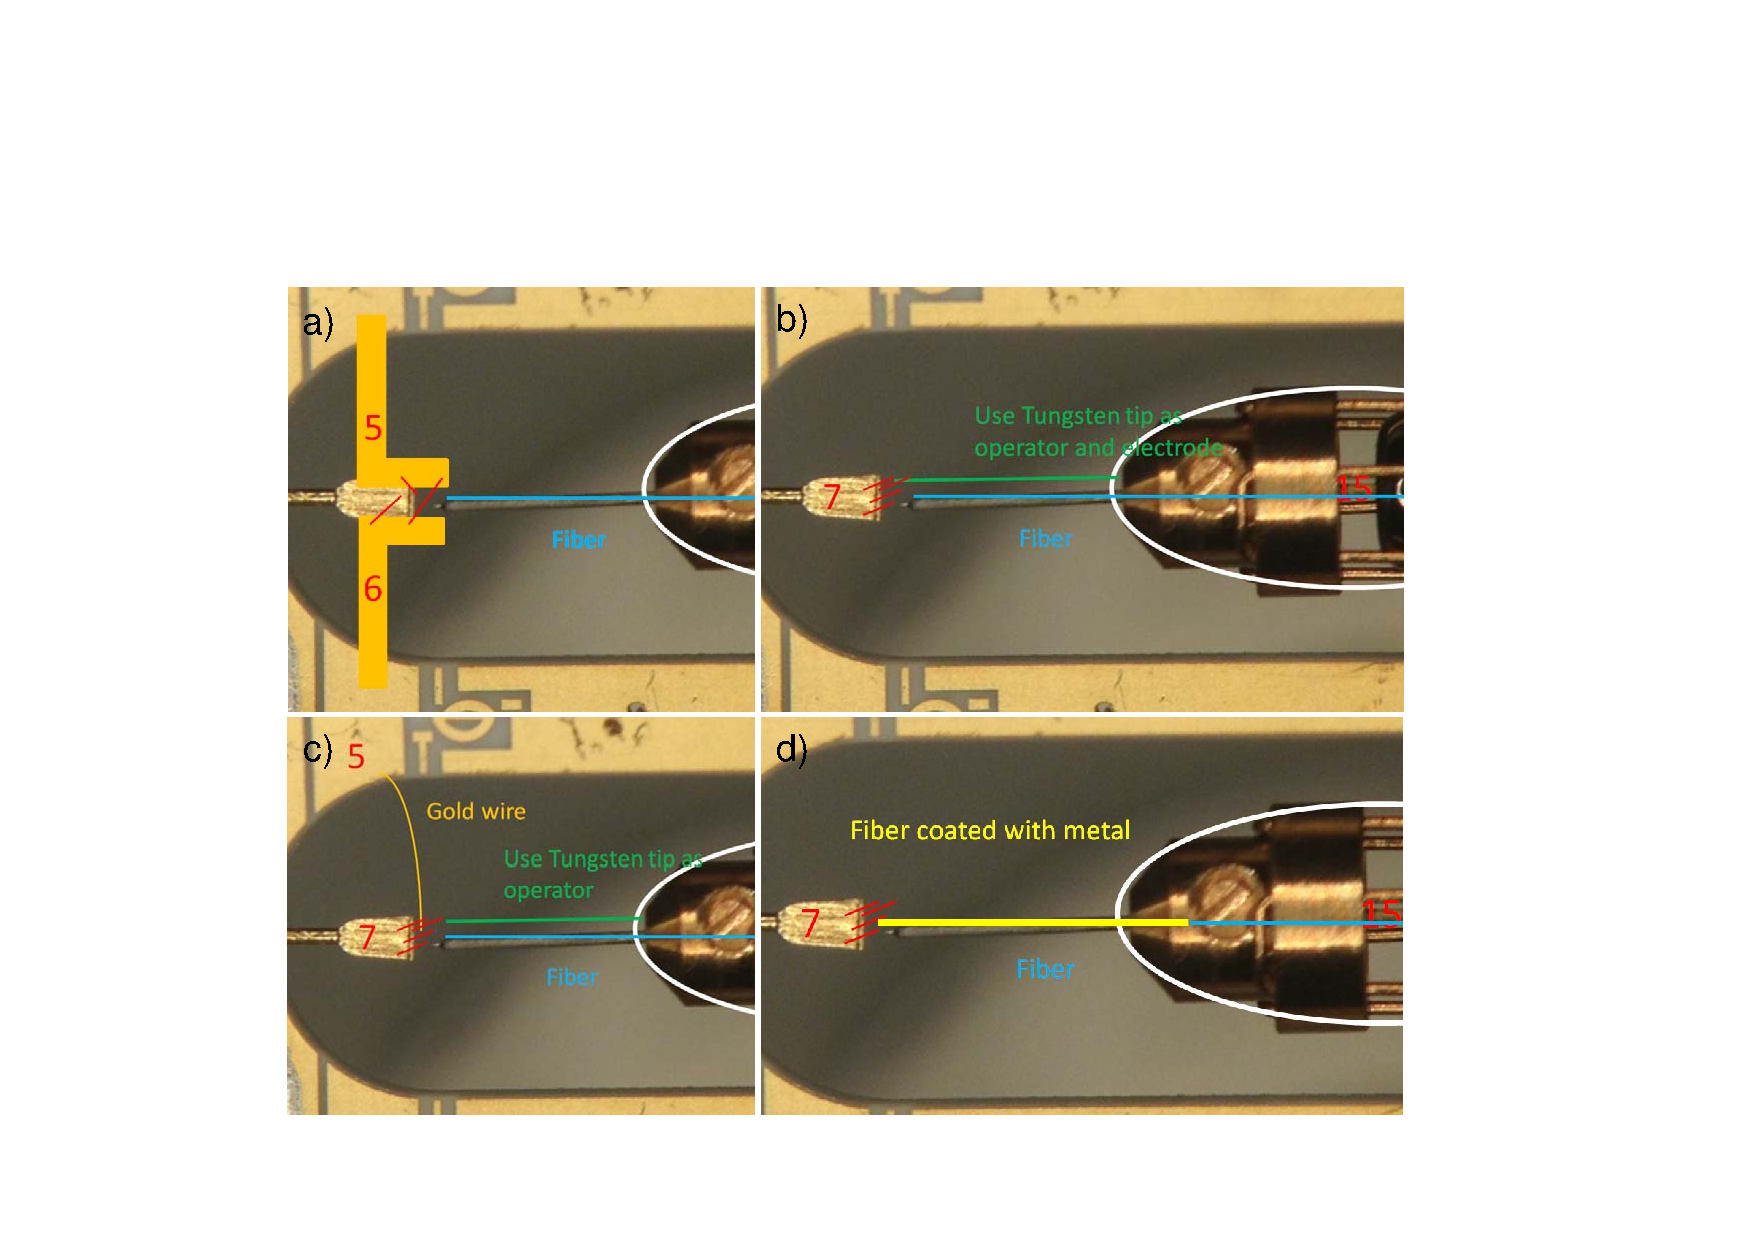
\includegraphics[height=0.95\textwidth, angle=-90]{figures/figure2_4ways}
\caption[Proposed four ways of holder adaption]{Four schemes I proposed for introducing probing functions into the optical holder.
\label{fig:4ways}}
\end{figure}

A multimodal optical nanoprobe allows scientists to perform standard experiments natural for TEM in addition to those involving optical excitation and measurements on the sample, including electrical measurements, STM and combinations of those. They emphasized the ability to simultaneously measure optical and electrical properties of the sample at the nanoscale.\cite{Zhu2012Multimodal}  The operations introduced were very similar to our case, but their serious problems were related to the calibration of light spot location, which had been realized by the adjustment of the tiny mirror screws; also, they were not able to confirm the location of light spot. Therefore the system was not that practical. \\
Minor et al. have implemented an {\it in situ} TEM monitoring technique to observe the crystallization of a-Si during high power pulsed laser irradiation by directly coupling laser into a TEM through a fiber-optics probe. By realizing a near-field scanning optical microscopy (NSOM) fiber probe scheme, this technique opens up a wide variety of new characterization possibilities.\cite{Xiang2012}\\
Kociak et al. of the Université Paris-Sud \cite{Zagonel2011} developed a STEM-CL system on a \textit{Nion} microscope which also uses an optical fiber as a light guide from the microscope column to the CCD camera outside the microscope. The light is collected by the specially designed mirror system of which the focus point is on the specimen. This CL-STEM imaging can be applied to obtaining luminescence spectra and observing the structures simultaneously.\cite{Nagarajan2016Simultaneous}

\begin{table}[ht]
\centering 
\begin{tabular}{|c|c|c|c|c|} 
\hline 
Organization & Fiber & Through & Probing contact & Practical for\\ [0.5ex] 
\hline 
Nagoya U. & Yes & hole, holder direct & No & CL\\[1.5ex] 
BNL & Yes & holder by sides & Yes & N/A\\[1.5ex]
LBNL & Yes& holder direct & No & NSOM heating\\[1.5ex]
U. Paris-Sud & Yes & holder direct & No & CL-Map, NSOM\\[1.5ex]
ASU & Yes & detector/aperture & No & Photochem.\\[1.5ex]
NIMS & Yes & holder direct & Yes & all above\\
\hline
\end{tabular}
\caption{Comparison of the groups which introduced light to TEM} 
\label{table2.2} 
\end{table}

In another group, Miller in Prof. Crozier's group in Arizona State University replaced the EDS detector (first version) or objective aperture (second version on a FEI Titan microscope) with an optical fiber to shine a light onto chemicals to observe dynamics of photochemical reactions.\cite{Miller2012} 
But the problem was that they had not been sure about the location of the light spot, because they just could not observe it.

To conclude, by introducing light into TEM, these days, the researchers are capable of observing dynamics of photochemical processes or thermo-effects, and to simultaneously obtain high resolution CL with EELS and Dark field imaging. As summarized in Table \ref{table2.2}, almost all groups used optical fibers for introducing light rather than lens system on bench, whereas most groups do not offer probing contact capabilities. In my case (NIMS in Table), I would like to realize all these functions based on the redesigned optical holder. 

\subsection{Our holder adaption}
To choose between the fiber technology and the breadboard, it is necessary to define the objectives and a budget. 
A honeycomb core breadboard is a complex and powerful layout to customize optical input/output parameters with high precision. 

However, building of an optical system on a honeycomb core breadboard could be costly. 
At least one optical window should be opened on the body of a microscope, so as to transmit an aligned laser beam into the chamber, and to collect optical signal from it. 
In contrast, by using an optical fiber, a laser light could be easily introduced into the microscope without breaking the TEM column. 
The solution is to make a continuous hole through a special TEM holder, so as to insert an optical fiber in it. The former {\it Nanofactory Instruments AB} developed a holder for our Laboratory with a 250 micrometer pipeline. 

In our system, the microscope is not modified at all, and we integrate all the experimental dynamics through the specimen holder. 

The front frame of the special holder was placed into the 4 mm gap of the TEM pole
piece. And with the optical fiber inserted, the light connection between the TEM chamber and the outer space was realized. 

To develop the whole system based on the regarded general idea, the two issues for the setup should be of our prime concern. One issue is the inner TEM side – how to place the samples, how to design the fiber tip, how to operate and apply/test electrical signals on the samples. The other side is the outer TEM side – board development, space for light source and signal processing.  

\begin{figure}  
\centering
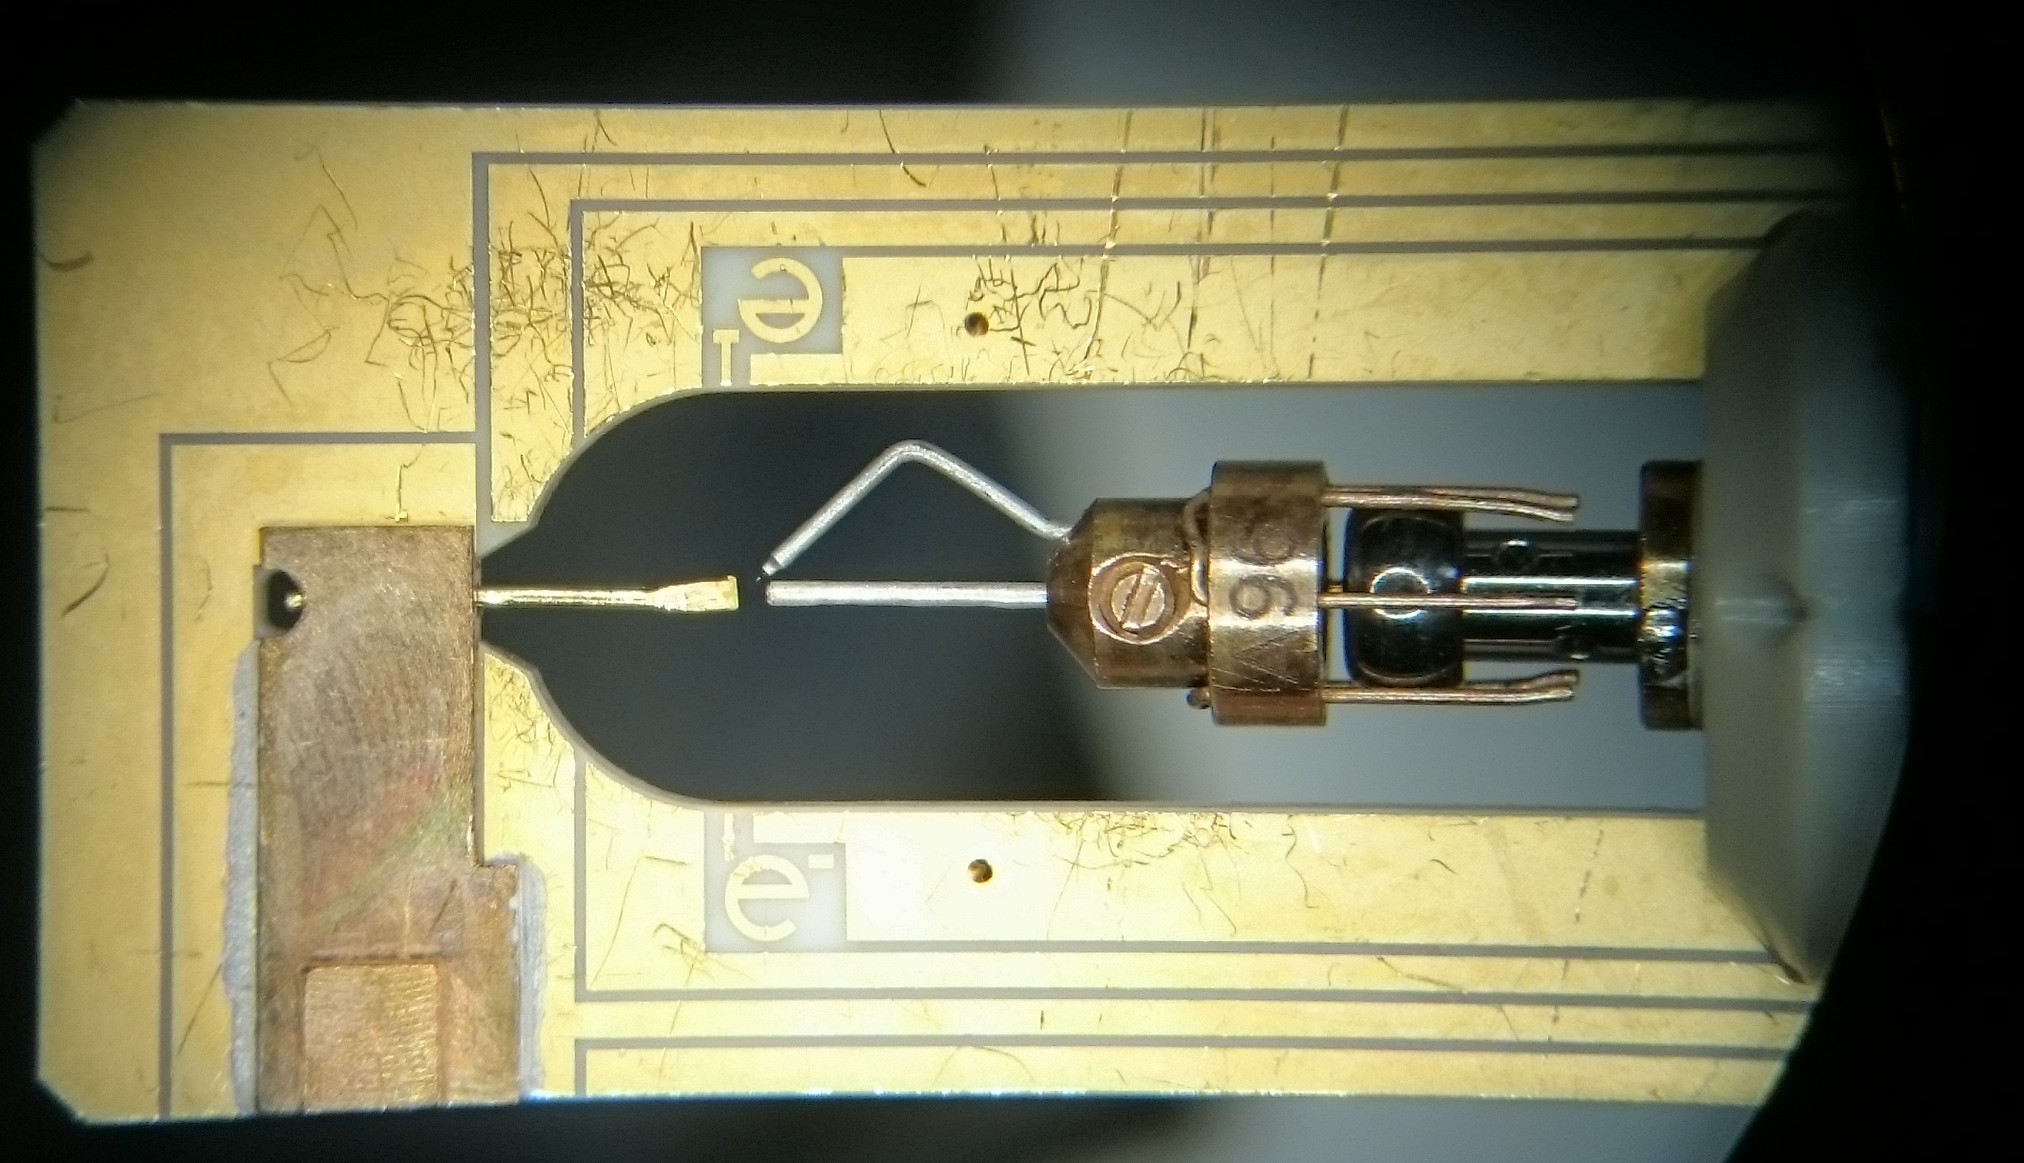
\includegraphics[width=0.7\textwidth]{figures/figure2_holderframe}
\caption[Inner part of the holder]{The part of a holder inside the pole-piece of TEM to illustrate geometrical relationship between sample stage, probe, fiber and electron beam.
\label{fig:2_frame}}
\end{figure}

I proposed 4 ways to add electrical capabilities to the piezo-driven optical holder based on the \textit{Nanofactory} optical holder, as shown in Figure \ref{fig:4ways}. 
The are namely: \\
\begin{itemize}
	\item[a)] To build the separated arms on the frame and to place a sample across the arms (this can be very difficult) where it can be illuminated; 
	\item[b)] To drill a hole on the original cap, or to make a new hat with two holes and to install an additional probe; 
	\item[c)] Based on design b), one end of a gold wire can be placed on the electrical pad using a wire bonding machine, the other end of wire can be manipulated to make contact with the specimen, therefore, in total three electrodes become available; 
	\item[d)] To coat a conductive metal onto the surface (cross section is not affected) of the optical fiber (which is marked in yellow), the coating electrically joins the end (edge) of the fiber and the cap (an electrode); 
\end{itemize}
The possible ideas are not limited by these four ways. Combinations of a) and b), or a) and d) are also possible. By building arm(s), installing probe(s), bonding wire(s) and coating conducting layers, electrical probing can enrich the functionality of the optical holder. 

Considering the fact that attaching a probe onto the piezotube driven hat would enable more dynamic options available for our microscopy, I finally decided to drill a hole on side of the hat and to attach an additional metallic probe to it, while at the same time to coat a gold layer onto the fiber tip to reduce fiber charging during its exposure to an electron beam. 

\begin{figure}  
\centering
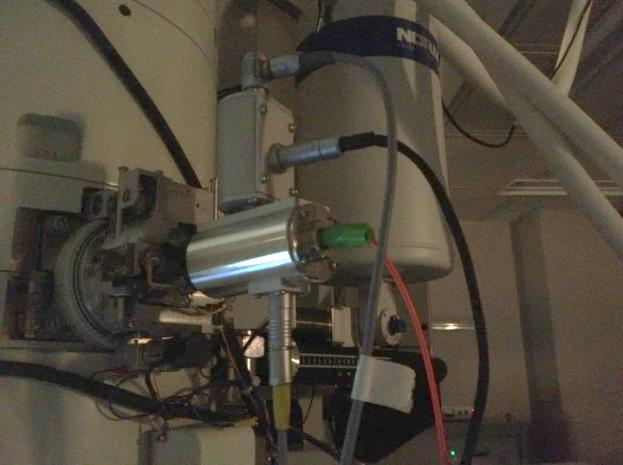
\includegraphics[width=0.7\textwidth]{figures/figure2_holderbot}
\caption[Outside of the holder]{The holder has several I/O ports for {\em in situ} mechanical, electrical and optical access.
\label{fig:2_bot}}
\end{figure}

For nanostructures, sampling is rather easy, the samples can be attached to the gold wire tip by touching, pressing, dipping or dropping, so that they could finally be exposed to an electron beam.
However, the optoelectronic {\em in situ} system could be more complex. The fiber tip inside TEM is clamped by a specialized cap which is driven by a XYZ-piezo controller. A tungsten probe for manipulation and electrical contacting is attached on the specialized cap manually. \\
Therefore, the sample is exposed to the electron beam and light, while, at the same time, it is controlled and connected by the stage (gold wire) and the tungsten probe. \\

For thicker samples, the specimens can be made by using a focused-ion beam (FIB) technique, or a half TEM grid may be used. 
The alignments of a sample, a fiber tip and the probe are quite important whereas rather difficult. If the fiber tip is far away from the sample, then the light will be divergent; this means that the power intensity of light could be reduced in progression. Since the tungsten probe will approach and connect the sample, the fiber tip should be as close as possible to the probe also. 

\begin{figure}
\centering
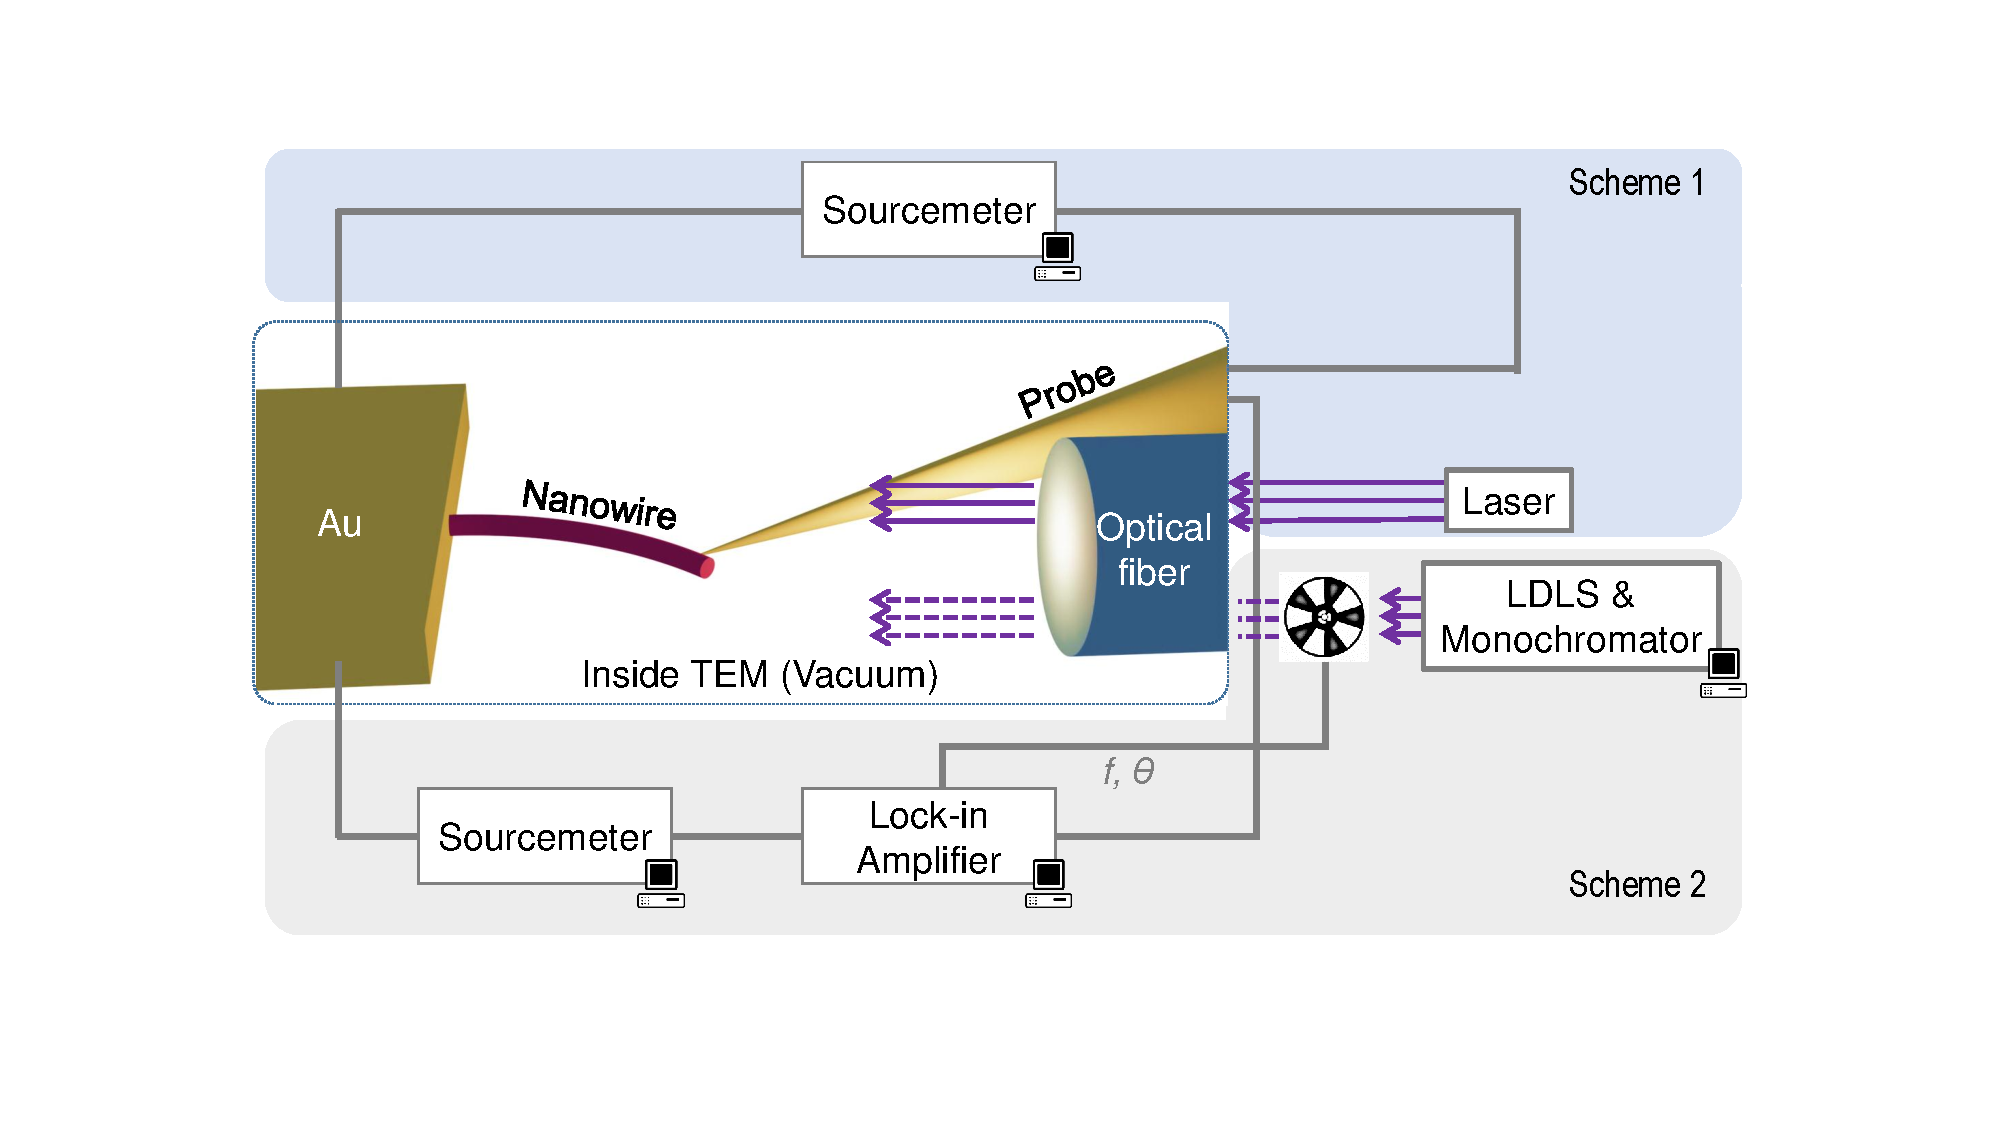
\includegraphics[width=\textwidth]{figures/figure6_1}
\caption[Optoelectronic {\em in situ} TEM scheme]{Optoelectronic {\it in situ} TEM scheme with two different light sources. }
\label{fig:6_1}
\end{figure}

In Figure \ref{fig:2_frame}, an image shows the geometrical relationship between the sample stage, probe, the fiber tip and electron beam. 

\subsection{Outer part of the microscope}
The individual coaxial electrical wiring through the holder for each contact gives pA level noises during the electrical measurements, allowing to measure low currents in Ohmic and non-Ohmic contact conditions. 

As shown in Figure \ref{fig:2_bot}, the holder has several ports for electrical, mechanical and optical signals to go in and out. 
The mechanical wire is at the downside, which is connected to the holder controller. 
The two electrical wires on top are connected to various electrical units depending on the experimental goal. 
At the bottom of the holder, optical fiber goes through and may serve as either a light source or a light detector, depending on application. 

A lock-in amplifier is used to extract a signal with an understandable carrier wave from a relatively noisy background. 
Because the light signal or photocurrent signal produced from a nanoscaled structure could be rather weak, detecting the signal against a bright noise could be accomplished using such amplifier. 
For example, in order to detect the photocurrents as a function of the wavelength of the incident beam one can apply a strong white light source, a chopper, a monochromator, a low-noise amperemeter and a lock-in amplifier, whereas the probe allows for measuring the electronic and optoelectronic responses. 

\begin{figure}  
\centering
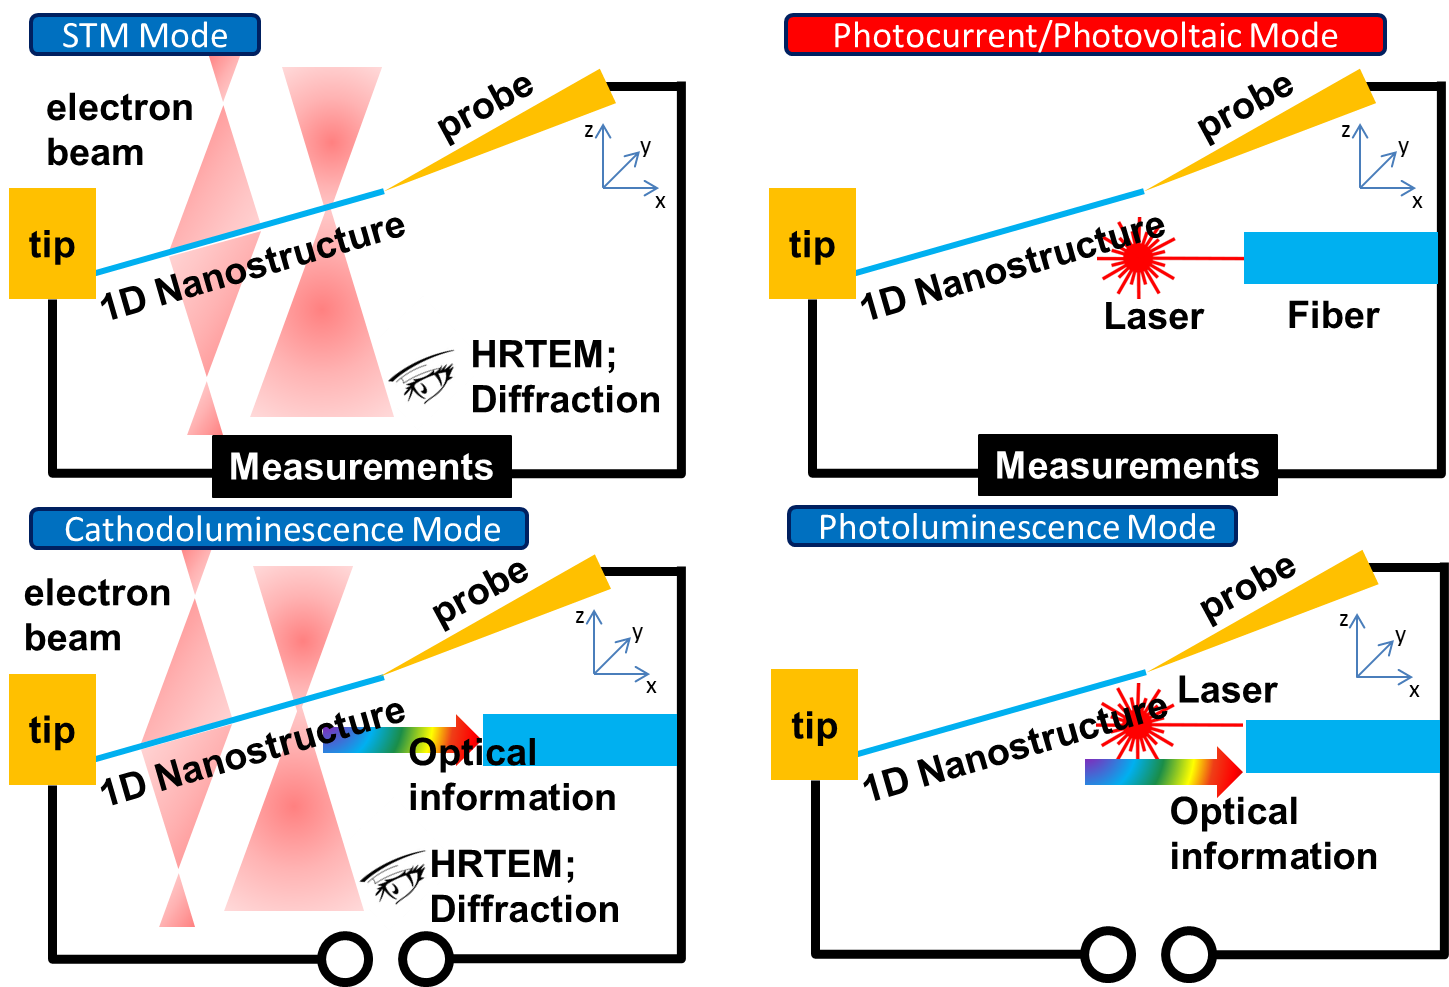
\includegraphics[width=0.9\textwidth]{figures/figure2_fourmodes}
\caption[Four modes]{Four modes of light-compatible {\em in situ} TEM.
\label{fig:2_fourmodes}}
\end{figure}

Thus, the optical {\em in situ} TEM system was developed and optimized by me during the last few years. It is now multi-functional: 
as shown in Figure \ref{fig:6_1}: the white light source and monochromator are used together with the chopper and lock-in amplifier to measure the photocurrents as a function of wavelength. The laser diodes and wave signal generator are used together with the lock-in amplifier to measure photocurrents and photovoltages at a certain wavelength. 

The final system is fully compatible with both the laser light source and other light sources such as the Lazer-Driven Light Source (LDLS, Energetiq Technology, Inc.) used by us. Usually, the white light source is utilized in tandem with a monochromator. 

\section{Applications and limitations}
\subsection{Applications}
 The interface morphology, the contact area and orientation, the material crystallography - all of these factors can precisely be determined under high resolution microscopy, while a bias and a light applied onto the sample. 

Four modes were designed for different purposes. These modes are demonstrated in Figure \ref{fig:2_fourmodes}.\\

The first mode is the conventional STM-TEM mode, which allows for controlling, measuring and observing a nanostructure. This mode is used to manipulate with the structures and to observe the samples for detailed imaging, including high-resolution imaging and diffraction analysis. 
The system is also capable for applying chemical functions to the specimen for electrochemical experiments inside TEM. \\

The second mode is thought to be the most effective one. Photocurrent and photovoltage could be measured in addition to the conventional STM-TEM mode.
However, in order to get rid of the influence of electron beam on the sample, it should often be moved away from the sample when measuring.\\

The third mode is the CL mode. On the opposite way, the optical signal could be obtained through the fiber tip when one applies an electron beam to the structures. By collecting the optical signal from a specimen through the optical fiber, spatially resolved CL information can be gained and correlated to the crystallography information. Also electrical biasing or current flow are optional in this mode. \\

The fourth mode is the photoluminescence mode. The interference is only happened when two coherent waves are superimposed. The system is not yet available, but it is possible to be established. 

\begin{figure}  
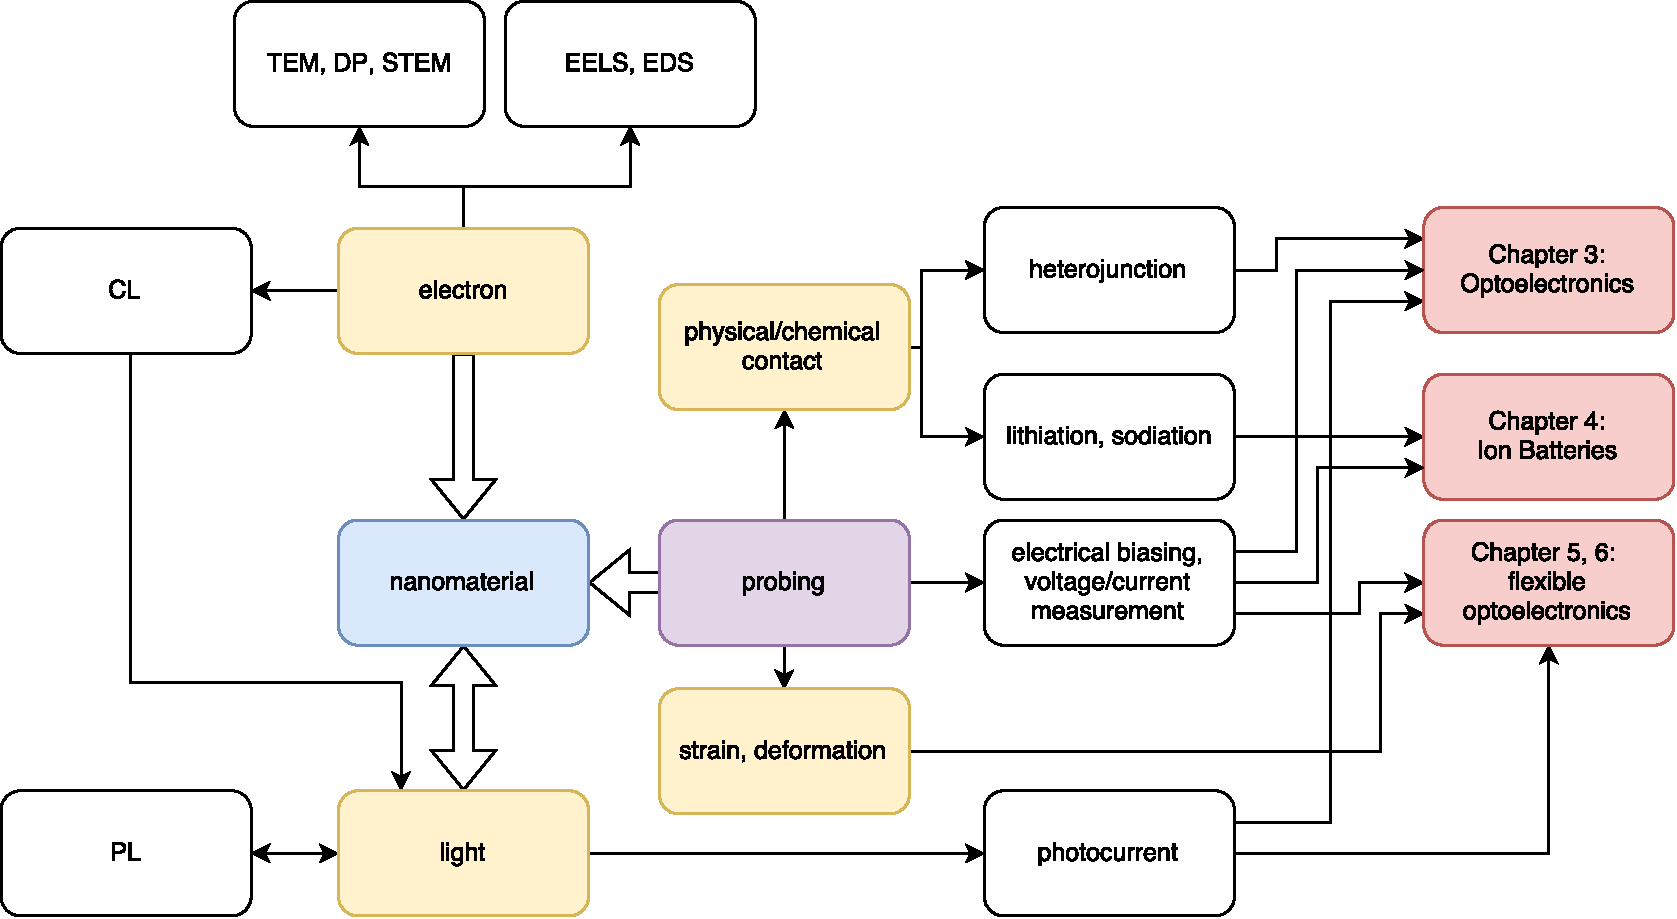
\includegraphics[width=\textwidth]{figures/figure2_apply}
\caption[Relationships between factors and applications.]{Relationships between factors and applications. Important dynamics is marked by yellow, some applications are marked by red, which will be detailed in other chapters.
\label{fig:2_apply}}
\end{figure}

In Figure \ref{fig:2_apply}, the relationships between all factors are presented. The applications of our light-compatible probing {\em in situ} TEM are not restricted to optoelectronics, flexible electronics/optoelectronics and lithium/sodium ion batteries, which are detailed in Chapters 3-6. More fields, such as a research on CL, PL, photovoltaic and photochemistry applications are expected to be explored in the nearest future. 

\subsection{Limitations}
First, the system is based on TEM, therefore, all limitations of TEM are also applied to our system; that is, the sampling requirement is strict, the sampling efficiency is low, TEM imaging gives only 2D information, and electron beam may either damage a specimen, or interfere the experiment. 

Secondly, the incident beam is limited by the properties of the optical fiber and the light source. The optical fiber is not easy to replace, and is not recommended to do this frequently. 
Also, the optical fibers always have their own band pass windows for light, as well as maximum power limitations. 
For special requirements, for example, for UV/NIR light experiments, a proper UV/NIR light source and a proper UV/NIR fiber are required, the polarization of light needs a special optical fiber, etc. 

Thirdly, the mechanical force is not measurable. Even though I list mechanics as one factor of the system, the mechanical information is quite limited and is only related to the manipulation. In fact, we are able to see a strain (and then evaluate the force by simulations, at least qualitatively) based on deviations on 2D TEM images or diffraction patters, but we are not able to measure the detailed force values or strain/stress distributions directly. 

However well designed experiments and professional manipulations can eliminate, or, at least, reduce the burden of the limitations mentioned above. 

%update: Jan 15 fixed figure/table numbers, fixed figure captions.  
%update: Jan 14 fixed grammar according to prof notes
%update: Jan 13 prof rewrite for ithenticate
%update: Jan 11 table 3.1 fixed
%update: Jan 09-11 prof check
%update: Jan 03 table ok. 
%update: Nov 21 fixed equation part. 
%update: Nov 09 by professor, rewrote all text. 

%\begin{savequote}[75mm] 
%It's rather easy to play any musical instrument: all you have to do is to touch the right key at the right time and the instrument will play itself.
%\qauthor{Johann Sebastian Bach} 
%\end{savequote}

\chapter{Nanoarchitechtonics of Axial Nanowire Junctions of CdS and p-Si}

\newthought{A high-precision technique} was implemented to build and analyze axial nanowire heterojunctions inside a high-resolution transmission electron microscope (HRTEM). Through {\em in-tandem} using of a sharp tungsten probe as the nanomanipulator and an optical fiber as the optical waveguide the nanoscale CdS/p-Si axial nanowire junctions were constructed, and \textit{in situ} recorded photocurrents from them were detected. Compared to the individual constituting nanowires, the CdS/p-Si axial nanowire junctions exhibit a photocurrent saturation effect which protects them from damage under high voltages. In addition, a set of experiments demonstrates the clear relationship between the saturation photocurrent values and the incident light intensities. The applied technique is envisaged to be valuable for bottom-up nanodevice fabrications, and the documented photocurrent saturation feature should solve the Joule heating-induced failure problem in nanowire optoelectronic devices caused by a fluctuating bias. 

\section{Introduction}
These days, the the key progresses in nanoscale photonics and electronics are made thaks to the significant improvement of functional device performances. Nanowires, as prime building blocks in the bottom up technology, have been shown to be the key candidates for the next generation booming nanophotonic applications because of their good crystallinity, high carrier mobility, confinement effects and infinite possibilities of assembling any required architecture for diverse utilizations \cite{lieberprogramable2014,tsai2014,zhangx2014}. However, till now, fabrication of a desired nanoarchitecture employing nanoscale building blocks has been a challenge. Several nanowire-based devices, such as transistors \cite{577926446,577926447,577926448}, diodes \cite{577926449}, photodetectors \cite{577926451,577926452} and logic circuits \cite{577926453,577926454}, have successfully been constructed on substrates through diverse lithography techniques. By contrast, controlled manipulation with two or more individual objects with a nanoscale precision and on-site creation of axial heteroarchitectures made of them (for the immediate optoelectronic probing) has never been tried. Building of the regarded junctions and \textit{in situ} testing of their optoelectronic characteristics would be highly important in relation to the “nanoarhitectonics” concept and uncovering novel physical properties and phenomena.\\ 

Cadmium sulfide (CdS) is known as one of the key materials in heterojunction type solar cell because of its advantageous type II window band structure  \cite{577926455}. Also, it was shown that merging of CdS and Si materials results in a decent junction. Therefore, numerous new functions and  utilizations may be envisioned. In addition, a careful study revealed that CdS/p-type-Si junctions are basically better than CdS/n-type-Si junctions for rectifying properties because of their specific type II band structure \cite{577926457}. Nevertheless, reliable usage of these two "hot" optical materials, i.e. CdS and Si, is rather rare, because both junction constituents are not transparent to a solar light. And the normal layered structures are considered not to be efficient. In order to directly expose the heterojunctions to the light, a smart way is to build the nanowire array structures \cite{577926458,577926459}. In addition to the wide-spread core-shell nanowire ensembles, constructing axial nanowire heterojunctions by means of two semiconducting materials is a promising experimental route.\\

\begin{figure}  
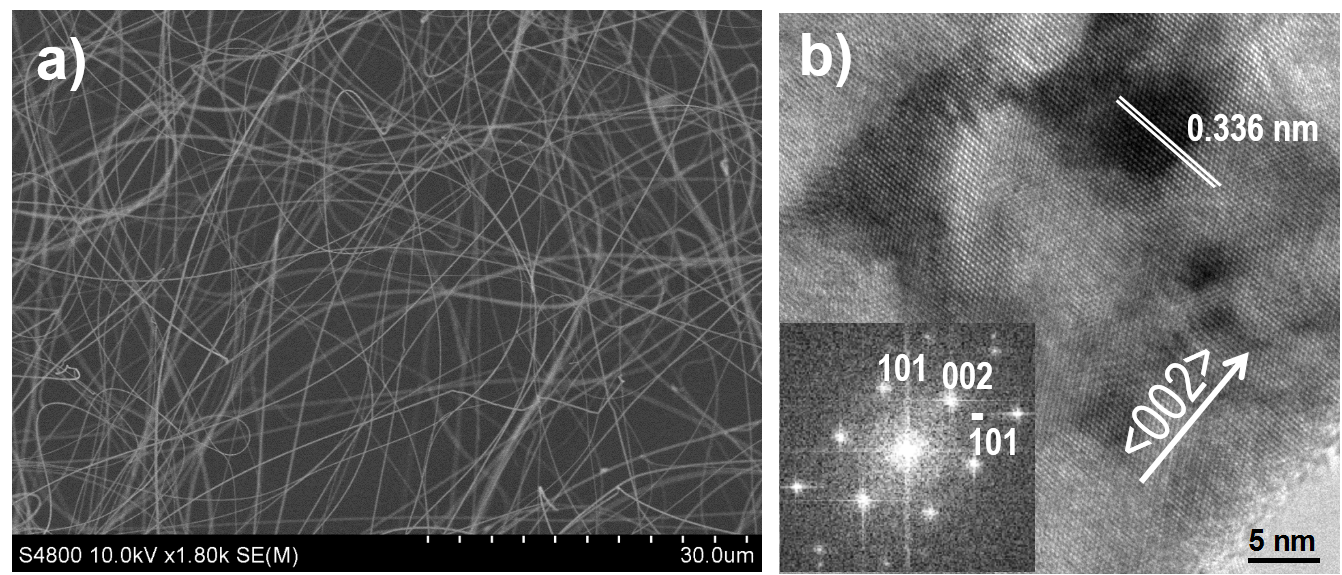
\includegraphics[width=\textwidth]{figures/figure3_s1}
\caption[SEM and TEM of CdS nanowires.]{(a) SEM image of CdS nanowires. (b) TEM image and corresponding fast Fourier
transform pattern of an individual CdS nanowire. 
\label{fig:fig3_s1}}
\end{figure}

Following previously made axial nanowire heterojunctions for diverse optoelectronic applications, CdS nanowires and B-doped Si nanowires have been selected by me as the targeting building blocks. Thus, in this Chapter, I demonstrate an accurate nanomanipulation technique pioneered in a HRTEM for building new axial nanowire architectures. Straightforward \emph{in situ} electronic and optoelectronic tests are then carried out on them using the light of various wavelengths shining into the TEM column. The designed experiments allow me to simultaneously have an entire control over the crystallography and spatially-resolved chemistry of the two constituting domains and their interfacial region before, during and after optoelectronic probing with high spatial and temporal resolutions specifically achievable with HRTEM. 
My experiments reveal clear photosensing properties of the axial CdS/p-Si nanowire junctions. The latter demonstrate selective sensitivity to blue and purple lights rather than to the light of larger wavelengths. Also, the junctions display a photocurrent saturation effect. This implies that such junctions are applicable in detecting light intensity due to their low energy consumption and stability under unexpectedly pulsing biases. 

\section{Experimental}
\subsection{Material Synthesis}

\begin{figure}  
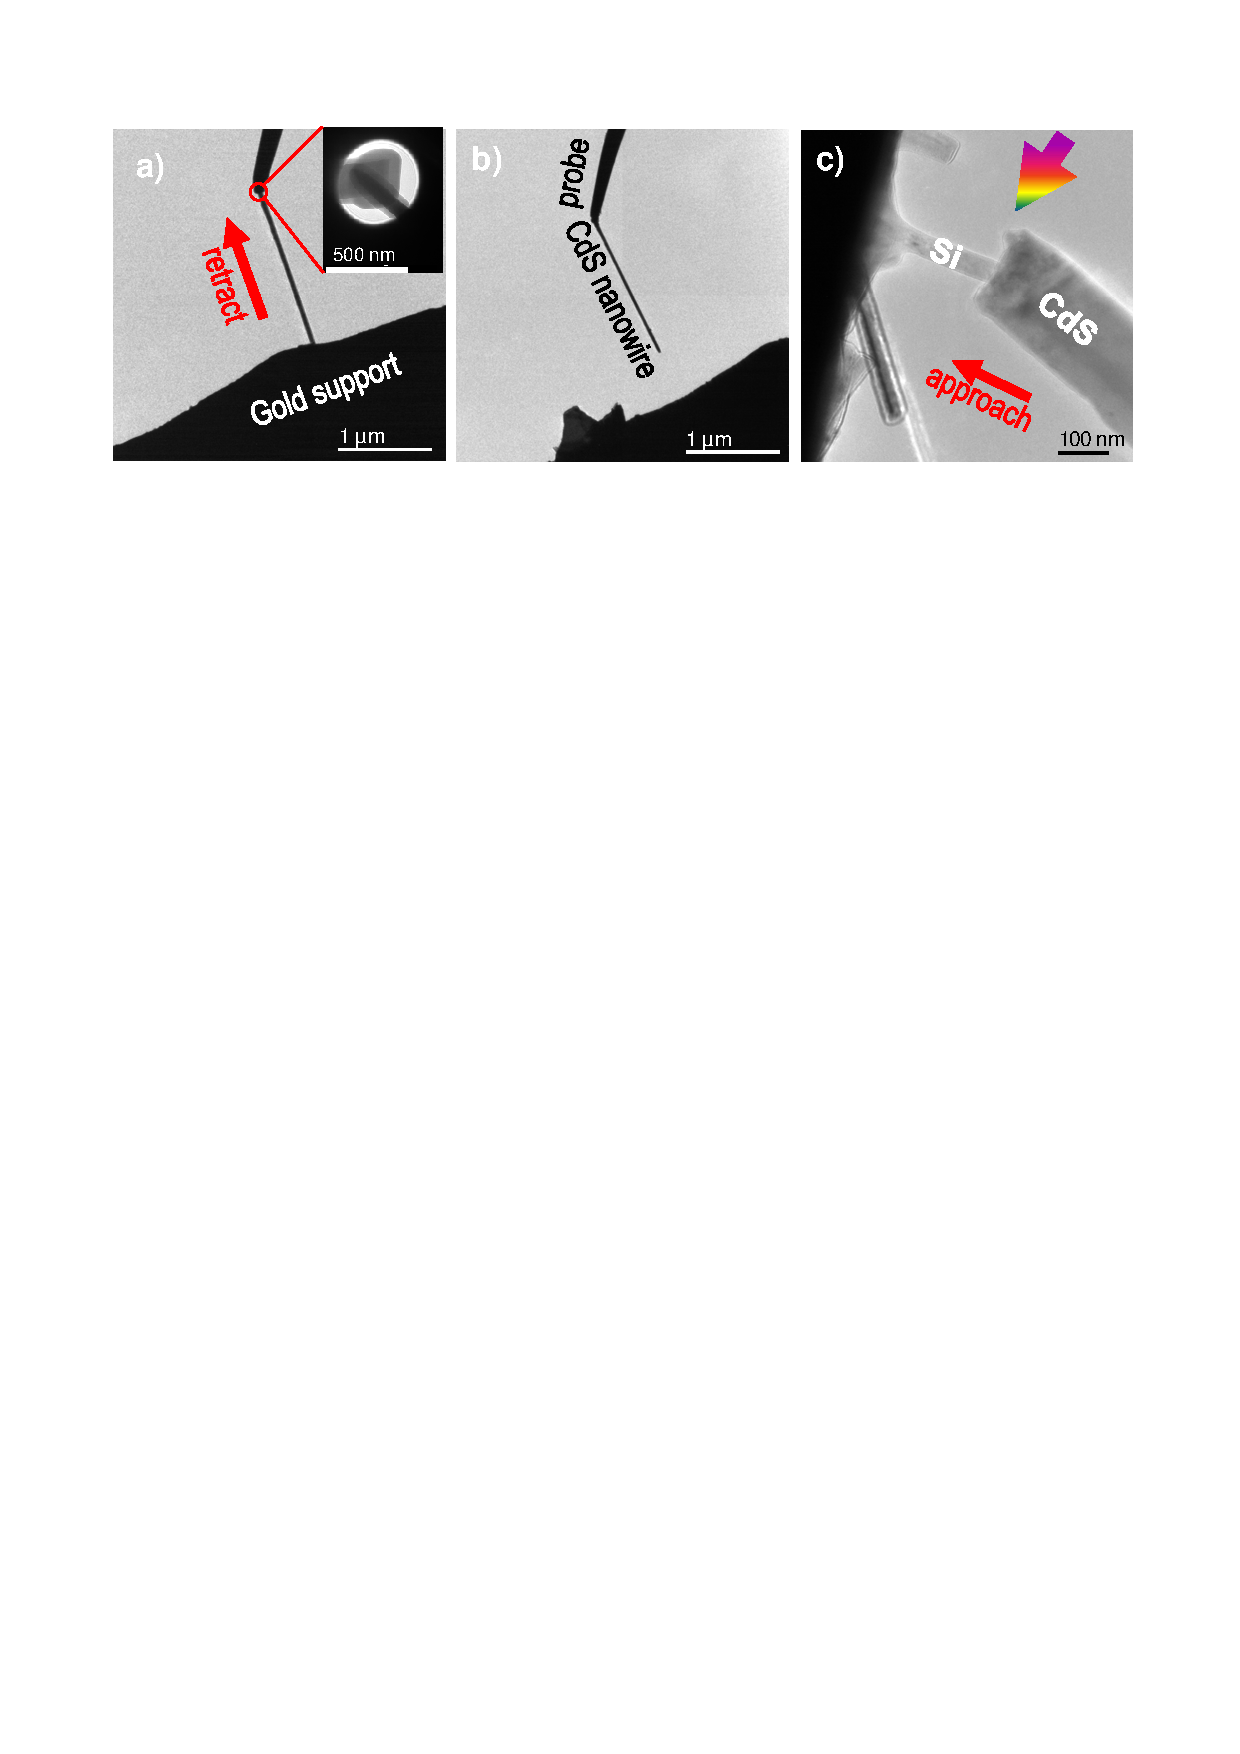
\includegraphics[width=\textwidth]{figures/figure3_1}
\caption[Making an axial junction.]{\textit{In situ} TEM images representing the fabrication process of an axial CdS/p-Si nanowire junction under manipulation in the electron microscope. (a) Making physical contact of a piezo-driven sharp tungsten probe with an individual clean CdS nanowire on a gold support during the first step of the manipulation; the inset shows soldering the tungsten probe and the wire under focused electron beam irradiation. (b) Pulling away the nanowire from the gold support; (c) connecting a CdS nanowire to the individual B-doped Si nanowire during the second step of the manipulation. The incoming light shining on the junction is marked with an arrow.
\label{fig:fig3_1}}
\end{figure}

The CdS nanowires were prepared using an Au-catalyzed vapor-liquid-solid (VLS) growth  in a chemical vapor deposition (CVD) system, which is analogous to that used in many works \cite{zhang2014photosensing,577926461}. 1 gram of a CdS powder (99.995\%) was put on a graphite plate at the tube furnace center as the source material. A (100) Si wafer covered with a 10 nm thick Au layer was put on the other graphite plate located downstream, at a distance of 11.5 cm from the tube center. The tube was purged under nitrogen flow at 200 °C for 2 h, and then heated to 1000 °C at a rate of 30 °C per min. After 30 min of reaction, the furnace was naturally cooled down to room temperature. The process took place under a \ce{N2} flow of 300 sccm. A wool-like yellowish product was found on the Si substrate after cooling. 
Si nanowires were fabricated via VLS mechanism in a separate CVD system. Au particles of 3 nm in diameter were taken as a metal catalyst. The B-doped nanowires were directly prepared onto Au-coated (111) Si substrates at 600°C for 30 min in a flowing 19 sccm of \ce{SiH4} as a Si reactant gas, and diborane (\ce{B2H6}) was employed as a B precursor. The \ce{B2H6} flow in \ce{H2} was 0.2 sccm and 30 sccm of \ce{N2} served as the carrier gas. Other details on B-doped Si nanowires characterizations were presented in the literature. \cite{577926462,577926464,577926465}.

\begin{figure}  
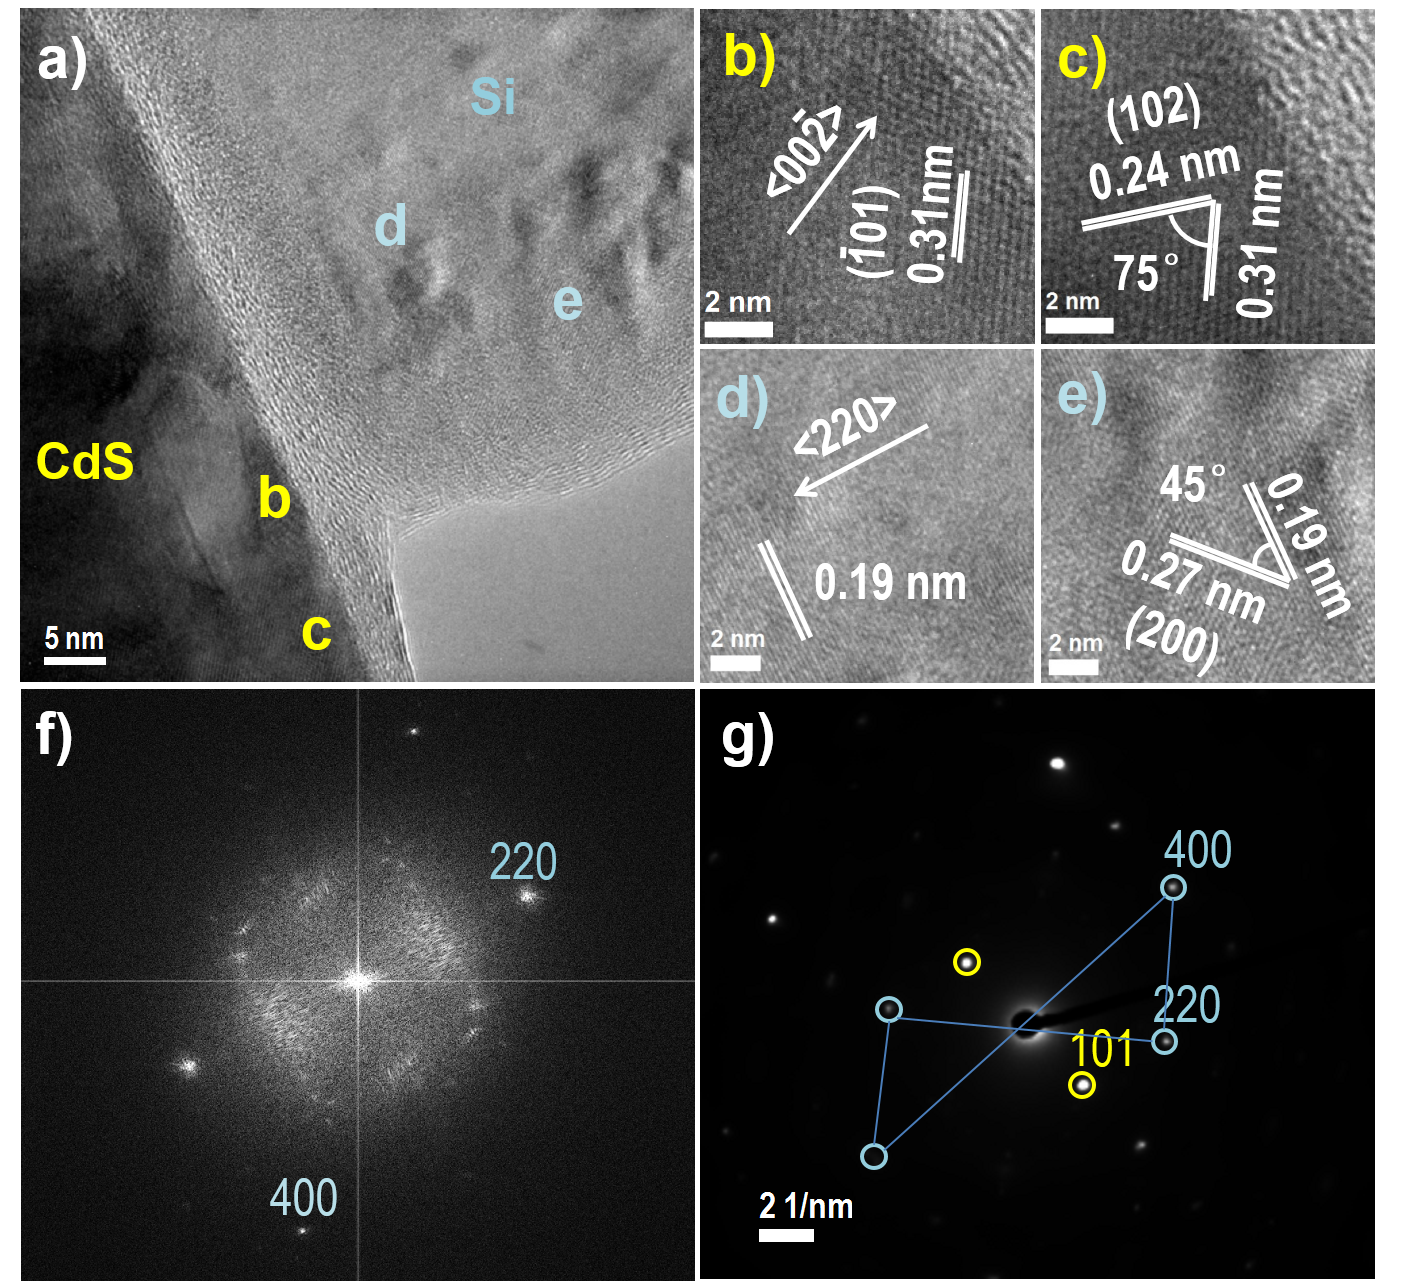
\includegraphics[width=\textwidth]{figures/figure3_2}
\caption[HRTEM anaysis on junction.]{(a) General HRTEM image of the interfacial area of the created CdS-p-Si junction; (b)–(e) HRTEM images taken in the areas marked in (a) showing the single-crystalline character of both nanowire branches, and (f), (g) corresponding FFT pattern and selected area electron diffraction pattern (SAED) taken from the interfacial region. Characteristic crystallographic directions (b)–(e) and reflections (f), (g) are marked.
\label{fig:fig3_2}}
\end{figure}

\subsection{Techniques}
Field-emission scanning electron microscopy (FE-SEM) of the prepared nanostructures was performed on a Hitachi S-4800 FE-SEM operated at 10 kV. HRTEM analysis and {\em in situ} experiments were carried out using an optimized piezo-driven optical TEM holder, which is discribed in detail in Chapter 2, in an energy-filtering 300 kV JEM 3100FEF (Omega Filter) high-resolution TEM. The multimode fiber (Nanonics Imaging, Ltd.) was threaded through the holder inner channel. The fiber was connected to four laser diodes, with 405, 488, 638 and 808 nm wavelengths, and a tunable power and temperature (Thorlabs, Inc.) were used. \\
The working temperatures of laser diodes were set at 30°C. Firstly, the numerous CdS nanowires were placed onto a fresh-cut flattened Au tip covered with an electrically conductive Ag epoxy under the flash tip immersing into the CdS nanopowder sample. After heating the paint, the Au tip with the specimen was placed within the sample holder. The ultrasharp W probes used as counter-electrodes and manipulators were prepared under NaOH electrochemical etching. The W tip movements were controlled inside TEM in 3 dimensions using a piezoelectric motor for making a contact, and to test and retract the selected CdS nanowires which had been conveniently oriented with respect to the manipulator. Then the fabrication of axial CdS/p-Si nanowire junctions was gently performed in two steps, as described in the following section. Typically, prior to contacting the two nanowire building blocks, an electron beam was applied to focus on the tip-ends of both CdS and p-Si nanowires for 30 s to clean the surfaces. The current–voltage (I–V) curves were recorded by using a Keithley 2612B sourcemeter. The electron beam was typically turned off during the electrical and optoelectronic tests. 


\section{Results and discussions}
As depicted in SEM image of Figure \ref{fig:fig3_s1}a, prepared CdS nanowires, $>50$ μm long, were evenly distributed over a Si substrate over a large area. In Figure \ref{fig:fig3_s1}b, a high-resolution TEM image and the fast Fourier transform pattern (FFT) confirm that an individual nanowire has a well-crystallized hexagonal structure. The growth direction is parallel to the $c$-axis and the lattice constant $c = 0.672$ nm. 

\begin{figure}  
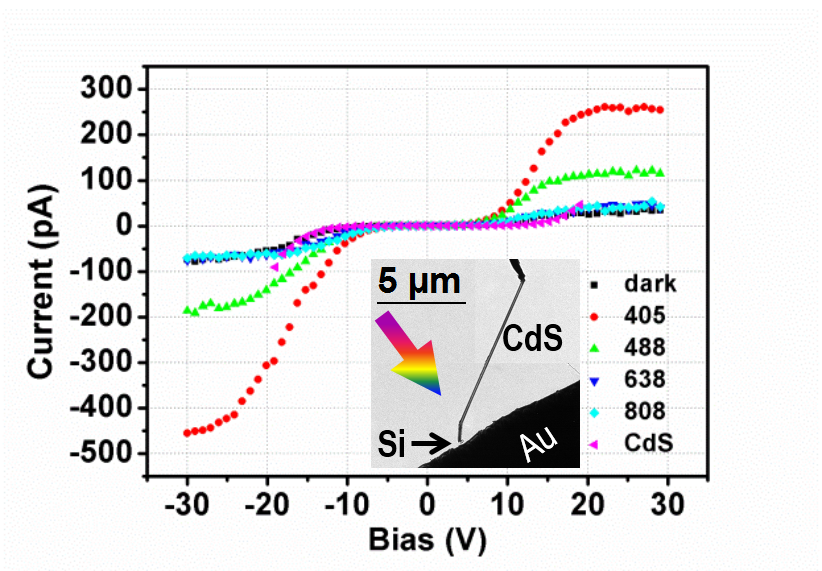
\includegraphics[width=\textwidth]{figures/figure3_3}
\caption[Photocurrent through junction.]{A photocurrent response of an individual CdS/p-Si axial nanowire junction under a dark condition and during illumination with the light of various wavelengths and with fixed intensity. The inset is the low-magnification TEM image of the CdS nanowire structure under testing. The colored arrow shows the incoming light incidence; the black arrow marks a short Si-branch segment.
\label{fig:fig3_3}}
\end{figure}

Because the deoxidized Si nanowires are less stable than CdS nanowires in air, for constructing heterojunctions, it was important to transfer a CdS nanowire into the HRTEM first, and then to contact a Si nanowire, not \textit{vice versa}. As shown in Figure \ref{fig:fig3_1}a, the sharp W probe was precisely manipulated inside HRTEM to contact a pre-selected clean individual CdS nanowire on the Au stage. To pull out the CdS nanowire from the sample stage, an electron-beam soldering, i.e. "glue" technique, was utilized for making the tight contact between the probe and the nanowire. \\

As illustrated in the inset of Figure \ref{fig:fig3_1}a, by focusing a convergent electron probe (about 500 nm in diameter) on the contact area for 20 min, nearly 75 nm thick layer of the residual amorphous carbon (always present in the TEM chamber from lenses, apertures etc.) formed on the probe/nanowire surfaces  resulting in their intimate nano-soldering. \\

Then, the targeted CdS nanowire was detached from the Au sample tip under delicate pulling back the W probe, as shown in Figure \ref{fig:fig3_1}b. To build a final heterojunction, the second step was to contact the pulled-out CdS nanowire with an individual pre-selected boron-doped-Si nanowire. To do so, after retracting the sample holder (with the regarded CdS nanowire on the tungsten probe) from the microscope, the gold sample stage with CdS nanowires was replaced in HRTEM by the fresh Au sample stage with attached numerous deoxidized B-doped Si nanowires. By precisely approaching and contacting the end of the CdS nanowire probe to a selected Si nanowire tip, the axial heterojunction architectures were formed. Figure \ref{fig:fig3_1}c depicts a typical CdS/p-Si axial nanowire junction. These representative CdS and Si nanowires have diameters of ~187 nm and ~46 nm, respectively. The electron beam intensity was immediately weakened after the junction had been constructed. This was done to avoid the nanostructure overexposure to the electron beam which would lead to insurmountable structural changes, e.g. formation of irradiation-induced defects in the material.

\begin{figure}  
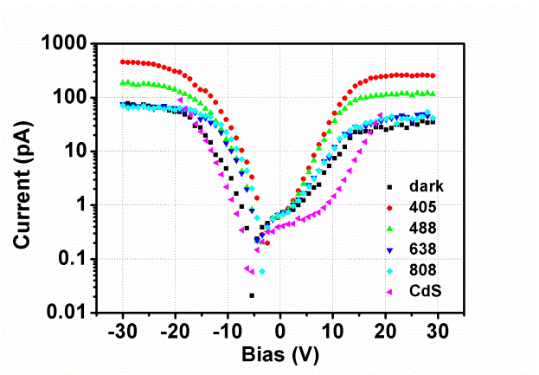
\includegraphics[width=\textwidth]{figures/figure3_4}
\caption[Photocurrent in Log scale.]{Photocurrent through junction in Log scale.
\label{fig:fig3_4}}
\end{figure}

Then, a detailed structural study of the junction was conducted using HRTEM imaging and electron diffraction analysis. The HRTEM images of a representative CdS/p-Si axial heterojunction are depicted in Figure \ref{fig:fig3_2}. These confirm that both nanowires are perfectly-structured single-crystals. The contact interface between two nanowires is atomically smooth. A thin transient graphitic layer is noticed between the wires. It has the origin similar to that mentioned above. In Figure \ref{fig:fig3_2}a, the left-hand-side panel shows the CdS nanowire, whereas the right-hand-side depicts the B-doped Si nanowire. Figures \ref{fig:fig3_2}b and \ref{fig:fig3_2}c present the entire crystallography of the CdS branch. Figure \ref{fig:fig3_2}d and \ref{fig:fig3_2}e present the crystal lattice of the constituting Si nanowire. Figure \ref{fig:fig3_2}f is the fast Fourier transform pattern of Figure \ref{fig:fig3_2}a. Figure \ref{fig:fig3_2}g is the selected area diffraction pattern taken at the junction interfacial region. After the complete structural analysis, which confirmed that high-quality axial heterojunction, constructed of two defect-free pure nanowire single crystals, had indeed been prepared, electrical and optoelectronic tests on it were promptly started. 

\begin{figure}  
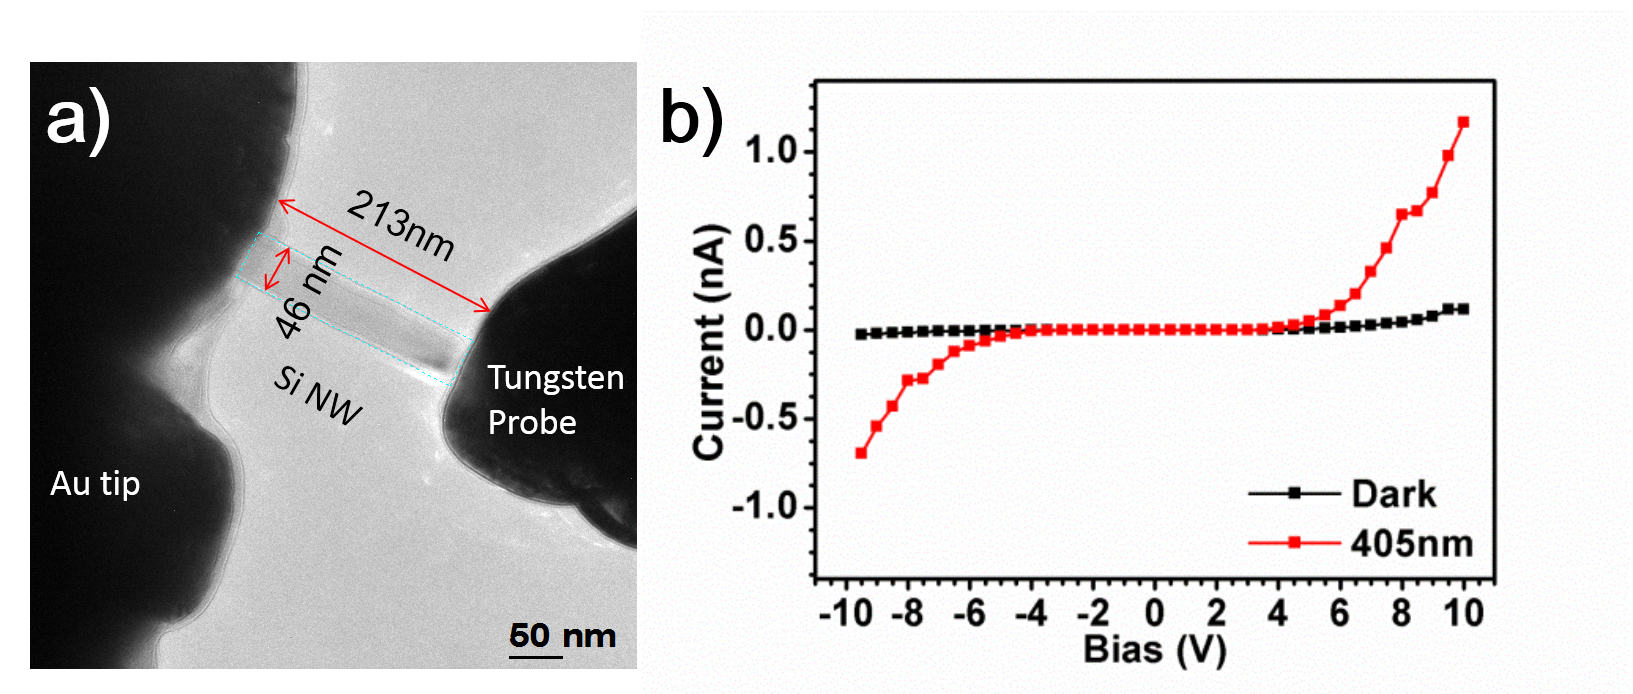
\includegraphics[width=\textwidth]{figures/figure3_s2}
\caption[TEM and currents of a Si NW]{(a) In situ alignment of a single B-doped Si nanowire for photocurrent measurements. (b) Dark current and photocurrent from the nanowire. 
\label{fig:fig3_s2}}
\end{figure}

While applying a bias and illuminating the preformed CdS/p-Si heterojunction with a light through the optical fiber threaded inside the holder, dark current and photocurrent data were collected. Figure \ref{fig:fig3_3} and Figure \ref{fig:fig3_4} illustrate a typical current – voltage diagram of a junction illuminated with lasers of 4 different wavelengths. The powers of all laser diodes were fixed to be the same, 13 mW. A photocurrent from the junction at 405 nm was larger than that at 488 nm, and much higher than those at 638 nm, and 808 nm, and the dark current. Because laser diode wavelengths of 405 nm, 488 nm, 638 nm and 808 nm correspond to energies of 3.06 eV, 2.54 eV, 1.94 eV and 1.53 eV, respectively, while CdS and Si nanowire band gaps are ~2.4 eV and ~1.5 eV, respectively, \cite{Fabbri2014}, the heterostructure light absorption at 3.06 eV and 2.54 eV must be easier than that at the energy below 2.4 eV. The higher photoresponse at 3.06 eV than that at 2.54 eV could reflect a complex band diagram of the heterostructure which gives more light absorption possibilities at the higher energy, and hence results in more photo-induced carriers. 


The I-V curves of the CdS/p-Si axial junction, where CdS is considered to be an n-type semiconductor (due to S vacancies), and B-doped Si as a p-type semiconductor, did not display an ideal p-n junction parameters. In the forward bias regime, below 10 V, the I-V curves reveal small currents, and the currents become saturated at a bias higher than 20 V. In the reverse bias regime, the currents also exhibit a saturation tendency, over 30 V. 

\begin{figure}  
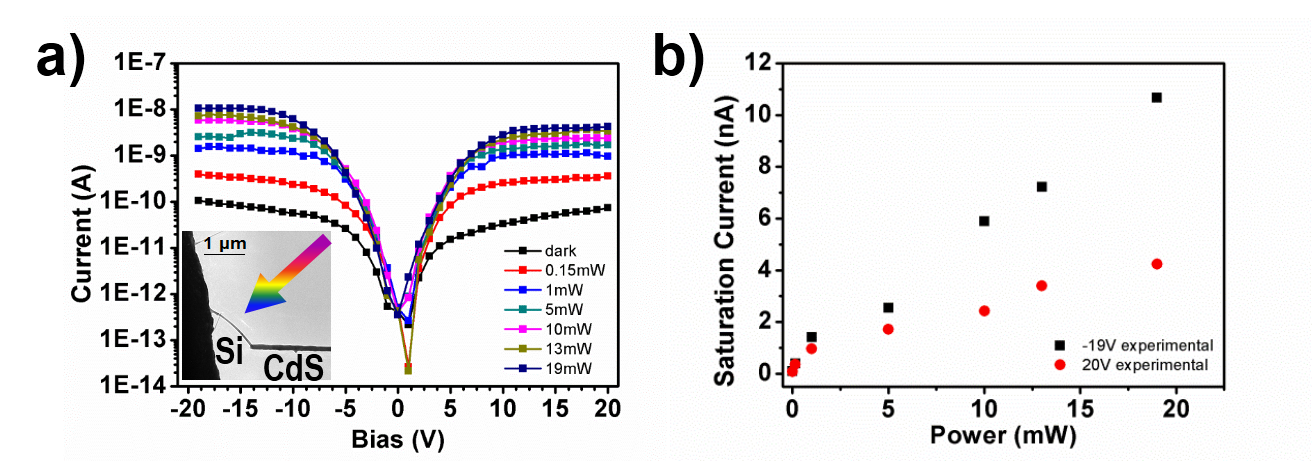
\includegraphics[width=\textwidth]{figures/figure3_5}
\caption[Photocurrent at different power]{Saturation of the photocurrent and dark current at different levels of light intensity. (a) Current–voltage plots at various laser powers; the inset shows the low-magnification TEM image of the structure under the measurements; the colored arrow illustrates the light incidence; (b) current-laser power plots at the two selected bias voltages.
\label{fig:fig3_5}}
\end{figure}

To compare, for an individual  CdS nanowire or a B-doped Si nanowire, saturation did not occur up to 10 V, as marked in Figure \ref{fig:fig3_3} and Figure \ref{fig:fig3_s2}. Once a bias larger than 10 V had been applied to a single CdS or Si nanowire, their structural breakdown readily happened. This was due to Joule heating at a high current density. \cite{Wu2004} In my experiments, the single crystalline nanowires (having narrow contact areas with the electrodes) were particularly vulnerable to current densities larger than ~104 $A\cdot cm^{-2}$. Therefore, it is apparent that the CdS/p-Si junction effectively hampered the current density at a high bias, and thus protected the structures from damage. 


Test experimental runs were performed to understand the associated factors responsible for the current saturation. As marked in Figure \ref{fig:fig3_5}, by recording  photocurrents for different light intensities at 488 nm, we observed that photocurrents and dark current of the CdS/p-Si axial nanowire junction at changing laser powers were saturated accordingly.The saturated currents were proportional to the laser diode power. Such phenomenon implies that the CdS/p-Si junction transfers light intensity into an electrical signal with the excellent voltage tolerance. As shown in Figure \ref{fig:fig3_s3}, another junction with a smaller contact area, which was illuminated by a 405 nm laser at 13 mW, also demonstrated a profound saturation effect. The photocurrent saturated at 5 V, the saturation current values were 15 nA and –75 nA. Therefore, it is likely that the junction contact conditions largely affect the saturation threshold and the current value. Generally, the photocurrents of nanowire photodetectors are proportional to the voltage \cite{577926470}, while, at the same time, they are proportional to the light intensity. This means that the voltage should be certain and stable within a limited tolerance for reliable light detection. Consequently, the presently built CdS/p-Si axial nanowire junctions show a great promise toward light intensity sensing not only because they can restrict the current density at a high voltage, but also because they do not need an entirely stable voltage. 

\begin{figure}  
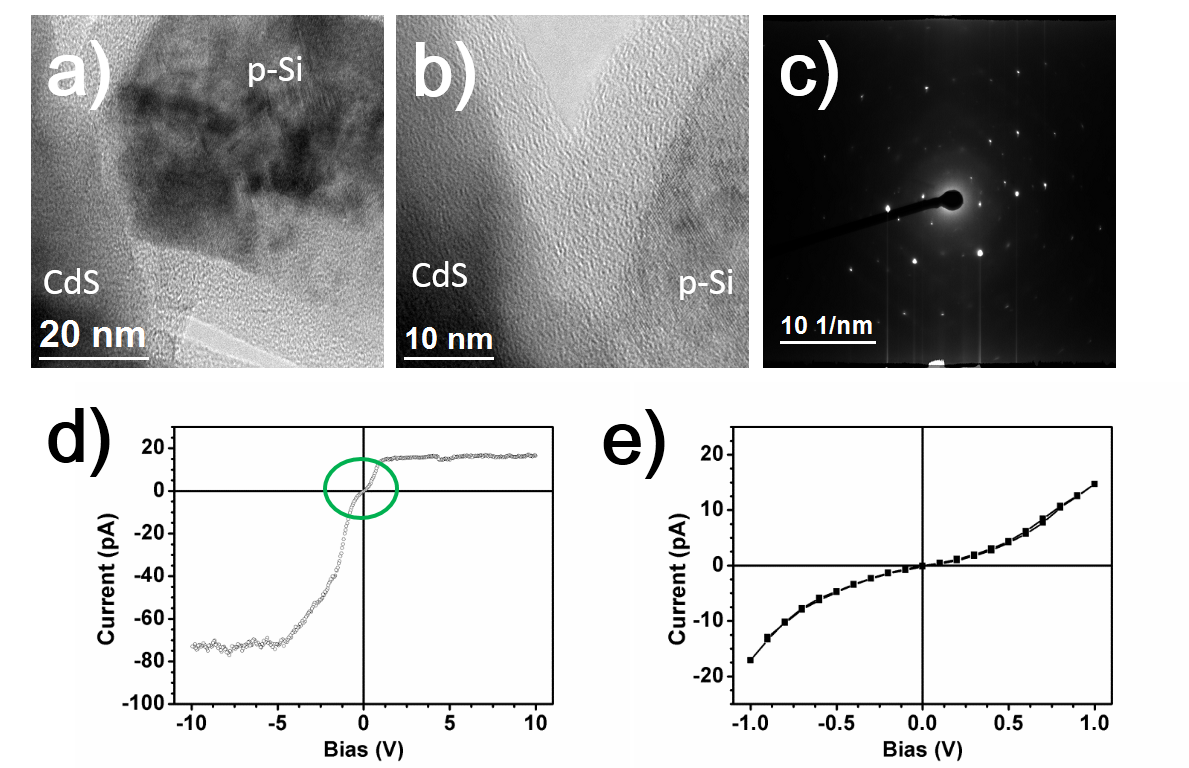
\includegraphics[width=\textwidth]{figures/figure3_s3}
\caption[Another junction]{ (a,b) TEM images, and (c) SAED pattern of a CdS/p-Si junction having the narrow contact region. (d-e) Photocurrent measurements on this junction. 
\label{fig:fig3_s3}}
\end{figure}

The observed phenomenon of photocurrent saturation at the high bias levels seems to to be analogous to that discovered for a planar Metal-Semiconductor-Metal (MSM) photodetector \cite{577926472}, electron beam excited CdS single crystals \cite{Dervos2004}, a model p-n junction \cite{577926474} and a p-n junction solar cell \cite{Gu2005}. Firstly, the electron beam excitation mechanism should be excluded, because the electron beam was shut during the measurements, and it did not have a continuous effect on a photocurrent of the material \cite{Dervos2004}. Secondly, the as-prepared CdS nanowires were confirmed to be defect-free single crystals with a marginal number of sulfur vacancies, and, hence, they did not operate as a heavily doped donor. For an ideal p-n junction, the dark current could be written as: 
$$I=I_s\left(e^\frac{V_D}{nV_t}-1\right)\eqno{(1)}$$

Equation ($1$) is named as Shockley’s diode equation \cite{577926477} and the dark current density of a non-ideal diode could be expressed as: 
$$J_F\approx-\frac{q(2D_p)N_i}{L_p}e^\frac{qV}{mk_0T}\eqno{(2)}$$
The factor $m$ in Equation ($2$) is changeable. Under circumstances of very low and very large biases, $m = 2$, and $J_F\propto e^\frac{qV}{k0T}$, the recombination current or the high injection takes an effect, current densities increase linearly; when bias is on a medium level, $m=1$, $J_F\propto e^\frac{qv}{2k0T}$, the diffusion current becomes important, and the current density exponentially increases. This is similar to the observed I-V curve trends, but Equation (2) does neither exactly explain the photocurrent saturation phenomenon nor the relationship between the saturation current value and incident light intensity. From the theory of photocurrent saturation developed by Mohammad and Abidi \cite{577926474}, for lightly degenerated semiconductors, where spatial variations of dielectric constant, effective mass, carrier lifetime, mobility and diffusivity are significantly small and could be neglected, the total current could be expressed as: 
$$I=Aqg\left ( L_{n}^{*}+L_{p}^{*} \right )-\frac{\left ( e^{\frac{qV_j}{kT}-1} \right )\cdot \left (  I_0+I_{0}^{'} e^{-z} \right )}{1-e^{-2z+z_1+z2}}\eqno{(3)}$$
where, 
$$I_0=\frac{qA}{\tau_a}(n_0(x_{p2})L_n^*+p_0(x_{n2})L_p^*)$$
$$I_0=\frac{qA}{\tau_a}(n_0(x_{p2})L_p^*e^{z2}+p_0(x_{n2})L_n^*e^{z1})$$
$$L_n^*=L_p^*=L_a=\sqrt{D_a\tau_a}$$
$D_a$, $\tau _{a}$ and $g$ are defined as ambipolar-diffusion coefficient, ambipolar lifetime and amibipolar-carrier generation rate in ref [33], respectively. We do not neglect injection, $V_j, V_d$, and  it is considered that $z_1=z_2=0$, $z=\frac{q}{kT}(V_d-V_j)$ in nondegenerated semiconductors with uniform doping, Equation (3) could be written as: 
$$I=2qAg\sqrt{D_a\tau_a}-k_v(n_0x_{p2}+p_0x_{n2})\eqno{(4)}$$
$k_v$ is defined as a factor to simplify the equation. The first term in the right-hand side of this formula represents the uncompensated current relative to light intensity, and the second term expresses the reduction of this photocurrent owing to spatial dependence of band structure of the junction and the junction potential produced by high injection. For a single B-doped Si or a defect-free CdS nanowire, the current densities increase with bias, as these do for a normal semiconductor nanowire with Schottky contacts. However, for the CdS/p-Si nanowire junctions with a limited junction area and under a large bias, the second term of Equation (4) becomes insignificant, and, therefore, the photocurrent does not increase with a bias but does with the light intensity. 
The observed saturation current values in correspondence with incident light intensities could be explained based on several factors. Because a sufficient bias must be applied to have the flat band at the anode and separate the generated carriers, after the threshold bias, the photocurrent started to notably rise, but when the bias is large enough, effective carriers generated by the incident light become saturated for transmission. In addition, we claim that the CdS/p-Si axial nanowire heterostructures are particularly sensitive to three factors: the relative sizes of the two building blocks (this affects carrier mobility), carrier density and light absorption efficiency; interface crystallography (which also affects mobility), junction parameters; and light intensity; which influences the photocurrent saturation value. 

%table with figure number
\begin{table}[ht]
\centering
\begin{tabular}{|c|c|c|c|c|c|}
\hline
Experiment No. & 1 & 2 & 3 & 4 & 5\\
\hline
CdS NW Length ($\mu$m) & 3 & 0.8 & 1.6 & 10 & 13\\
CdS NW Diameter (nm) & 240 & 38 & 135 & 187 & 120\\
Si NW Length ($\mu$m) & 0.9 & 1.5 & 1.3 & 0.2 & 1\\
Si NW Diameter (nm) & 55 & 44 & 44 & 46 & 63\\
Photoresponse detected & 26/26 & 22/22 & 16/16 & 57/57 & 16/16\\
Saturation current positive (nA) & 16 & 0.50 & 3.2 & 0.12 & 0.16\\
Saturation current negative (nA) & -27 & -0.69 & -7.2 & -0.19 & -0.2\\
\hline
\end{tabular}
\caption[Reproducibility of the saturation effect]{Five independent CdS/p-Si nanowire axial heterojunctions exhibiting the saturation effect all having varying values of sizes and currents. 
\label{table:3_1}}
\end{table}

Over this work I fabricated and thoroughly tested 5 distinct CdS/p-Si nanowire junctions. All of them exhibited the regarded saturation effects with somewhat varying parameters, as depicted in Table \ref{table:3_1}. The results imply that the saturation effect is natural and highly reproducible during \emph{in situ} TEM. 

\section{Conclusions}
To sum up, an original {\em in situ} HRTEM technique to construct individual axial nanowire junctions (perfectly emphasizing the modern {\em nanoarchitectonics} concept) has been demonstrated for the first time. 
{\em In situ} HRTEM and in-tandem structural characterizations and optoelectronic tests highlight the photosensing properties of the single-crystalline axial CdS/p-Si nanowire junctions. The junctions exhibit good selectivity toward the light frequencies higher than those of the yellow range. The junctions possess a specific photocurrent saturation effect; this could be utilized in low-consumption light intensity sensing and integrated tunable voltage-driven applications thanks to the corresponding current limitations and excellent tolerance toward possibly unreliable and unstable bias. \\
The developed nanoarchitectonics-based approach employing \textit{in situ} structural design and measurements gives a strong motivation for establishing new operational principles of single crystal nano-devices. 
Furthermore, it is also envisaged that the near-field scanning technique could be also integrated within the designed system for even better understanding of the exciting nanoscale optoelectronic phenomena.\cite{Gu2005,Xiang2012}.




%update: Dec 29 rewrite all. 
%update: Nov 21 citation done , figure done. 
%update: Nov 10 by zc, add more text(slightly edited), uploaded and compiled all figures. 
%update: Nov 09 by professor, rewrite the first half of text. 

\begin{savequote}[75mm] 
I am somewhat exhausted; I wonder how a battery feels when it pours electricity into a non-conductor?
\qauthor{Sherlock Holmes (Arthur Conan Doyle)} 
\end{savequote}

\chapter{\emph{In situ} TEM electrical probing for ultrastable sodium ion batteries}

\newthought{Sodium-ion batteries (SIBs)}, as an important alternative for future energy storage, have been on stage since 1980s. Among many anode materials, elemental phosphorus (P) has attracted most of the interest in recent years because of  large theoretical capacity, i.e. 2596 $mAh/g$. The prime disadvantage, however, of a P anode is its poor conductivity and fast structural degradation due to volume expansion, as much as $>$490$\%$, over working cycles. To address this issue, I redesigned the anode structure via fabricating a flexible paper made of amorphous P and N-doped graphene. The as-fabricated anode delivers ultrastable characteristics and superb rate capability, 809 $mAh/g$ at 1500 $mA/g$. The extraordinary structural integrity of this new anode was then studied via \emph{in situ} experiments inside a high-resolution transmission electron microscope (HRTEM), thereby the cyclic dynamics and sodiation/desodiation mechanisms were thoroughly understood. To confirm my experimental results, Density Functional Theory (DFT) calculations were additionally performed to indeed confirm that the N-doped graphene contributes to an increase in capacity for Na storage, and to an improved anode rate performance.

\section{Introduction}
Sodium ion batteries (SIBs) are receiving considerable attention and have bright expectations as one of the most promising alternatives to lithium ion batteries (LIBs) for energy storage.\cite{Ren2014c,Yang2011c,Liu2014a,Wen2014b,Shen2015b,wang2014e,Wu2014b,Yao2015b,Ni2014b} Both battery types possess analogous chemistry, but SIBs are cheaper because of more abundant sodium natural resources. In the recent reports, the cathode performance in SIBs was found to be comparable with that of the LIBs.\cite{Sun2014b,Barpanda2014b} However, such performance is still the major constraint for the immediate practical applications. There have been an increasing interest in developing high-power and high-capacity anode materials for the next generation SIBs,\cite{Ong2011b,Palomares2012b,Zhu2014b,Yu2014b,Berthelot2011b,Qian2012d,Wang2013g,Komaba2011b,Cao2012b,Wang2013h,Xu2013b,Qian2012e} such as transition metal oxides,\cite{Zhu2014b,Yu2014b,Berthelot2011b} Prussian blue analogues,\cite{Qian2012d,Wang2013g} hard carbon materials,\cite{Komaba2011b}, nanowires,\cite{Cao2012b} graphene,\cite{Wen2014b,Wang2013h}, tin composite, \cite{Xu2013b} and antimony-based materials,\cite{Qian2012e} but their specific capacities are still not competitive for future applications(<800 mAh/g). \\

\begin{figure}  
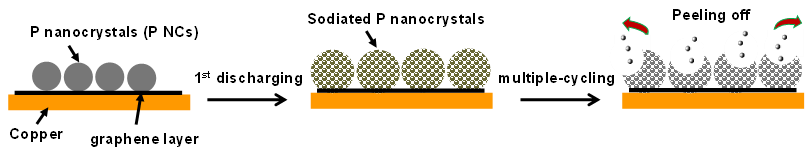
\includegraphics[width=\textwidth]{figures/figure4_s1}
\caption[Peeling off after cycling]
{Schematic diagram of the structural fracture of a high-volume-change type P anode, in which P nanocrystals anchored on the graphene layer are placed on the surface of a Cu current collector. After 1st discharging, there is a large volumetric expansion (>200-500\%) for P NCs; during cycling, such large volume change will lead to the pulverization and thus peeling off the electrode.
\label{fig:4_s1}}
\end{figure}

Among the hottest materials, elemental phosphorus (P) is one of the most attractive candidates with an ultra-high theoretical capacity of 2596 mAh/g\footnote{All capacities mentioned though the thesis are calculated based on the weight of composites.},\cite{Qian2013b,Kim2013c,Li2013c} i.e. about seven times higher than that of the commercial graphite anode in LIBs. The key challenge associated with a phosphorus anode is its rapid structural degradation caused by huge volume change (>490\%) under cycling. For conventional crystalline phosphorus (Figure \ref{fig:4_s1}), upon Na insertion, the P crystals are pulverized and thus the electrode film surface cracks (as a result of ~200-500\% volumetric expansion), leading to phosphorous peeling off from the current collector, which, in turn, gives a significant performance fading. So, stabilizing or sustaining the rigidness of the phosphorus anode structure during cycling is the practical key toward the improvement of the cycling performance of a P-based SIB anode. Very recently, notable breakthroughs have been witnessed in stabilizing anode structure through a design of amorphous P/carbon hybrids.\cite{Qian2013b,Kim2013c,Li2013c} For example, Qian et al. reported that the amorphous P/C hybrids prepared under high-energy mechanical milling had demonstrated a considerable capacity retention of 68\% after 60 cycles at the current density of 250 mA/g.\cite{Qian2013b} Kim et al. demonstrated that a similar amorphous P/C structure is able to deliver as high as 80\% reversible capacity and less than 7\% capacity fading after 30 cycles at a current density of 143 mA/g.\cite{Kim2013c} In addition, Chou et al. fabricated a composite anode via simple hand-grinding of commercial microsized red phosphorus and carbon nanotubes (CNTs); this demonstrated a high capacity retention of 76.6\% over 10 cycles.\cite{Li2013c} The improvements in cycling stability in the regarded reports were indeed remarkable, however, capacity retentions of less than 80\% still indicate that further developments are still needed in order to meet the practical requirements.\cite{Luo2015b}\\

\begin{figure}  
\centering
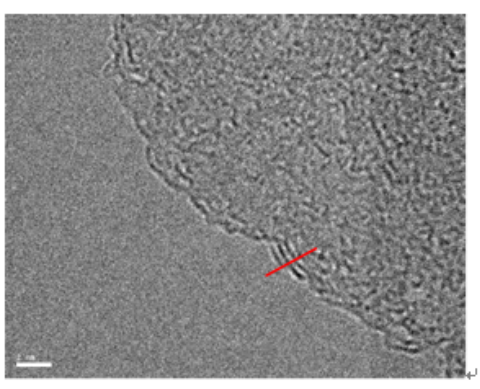
\includegraphics[width=300pt]{figures/figure4_s2}
\caption[TEM of GN]
{HRTEM image of an N-doped graphene (GN).
\label{fig:4_s2}}
\end{figure}

\begin{figure}  
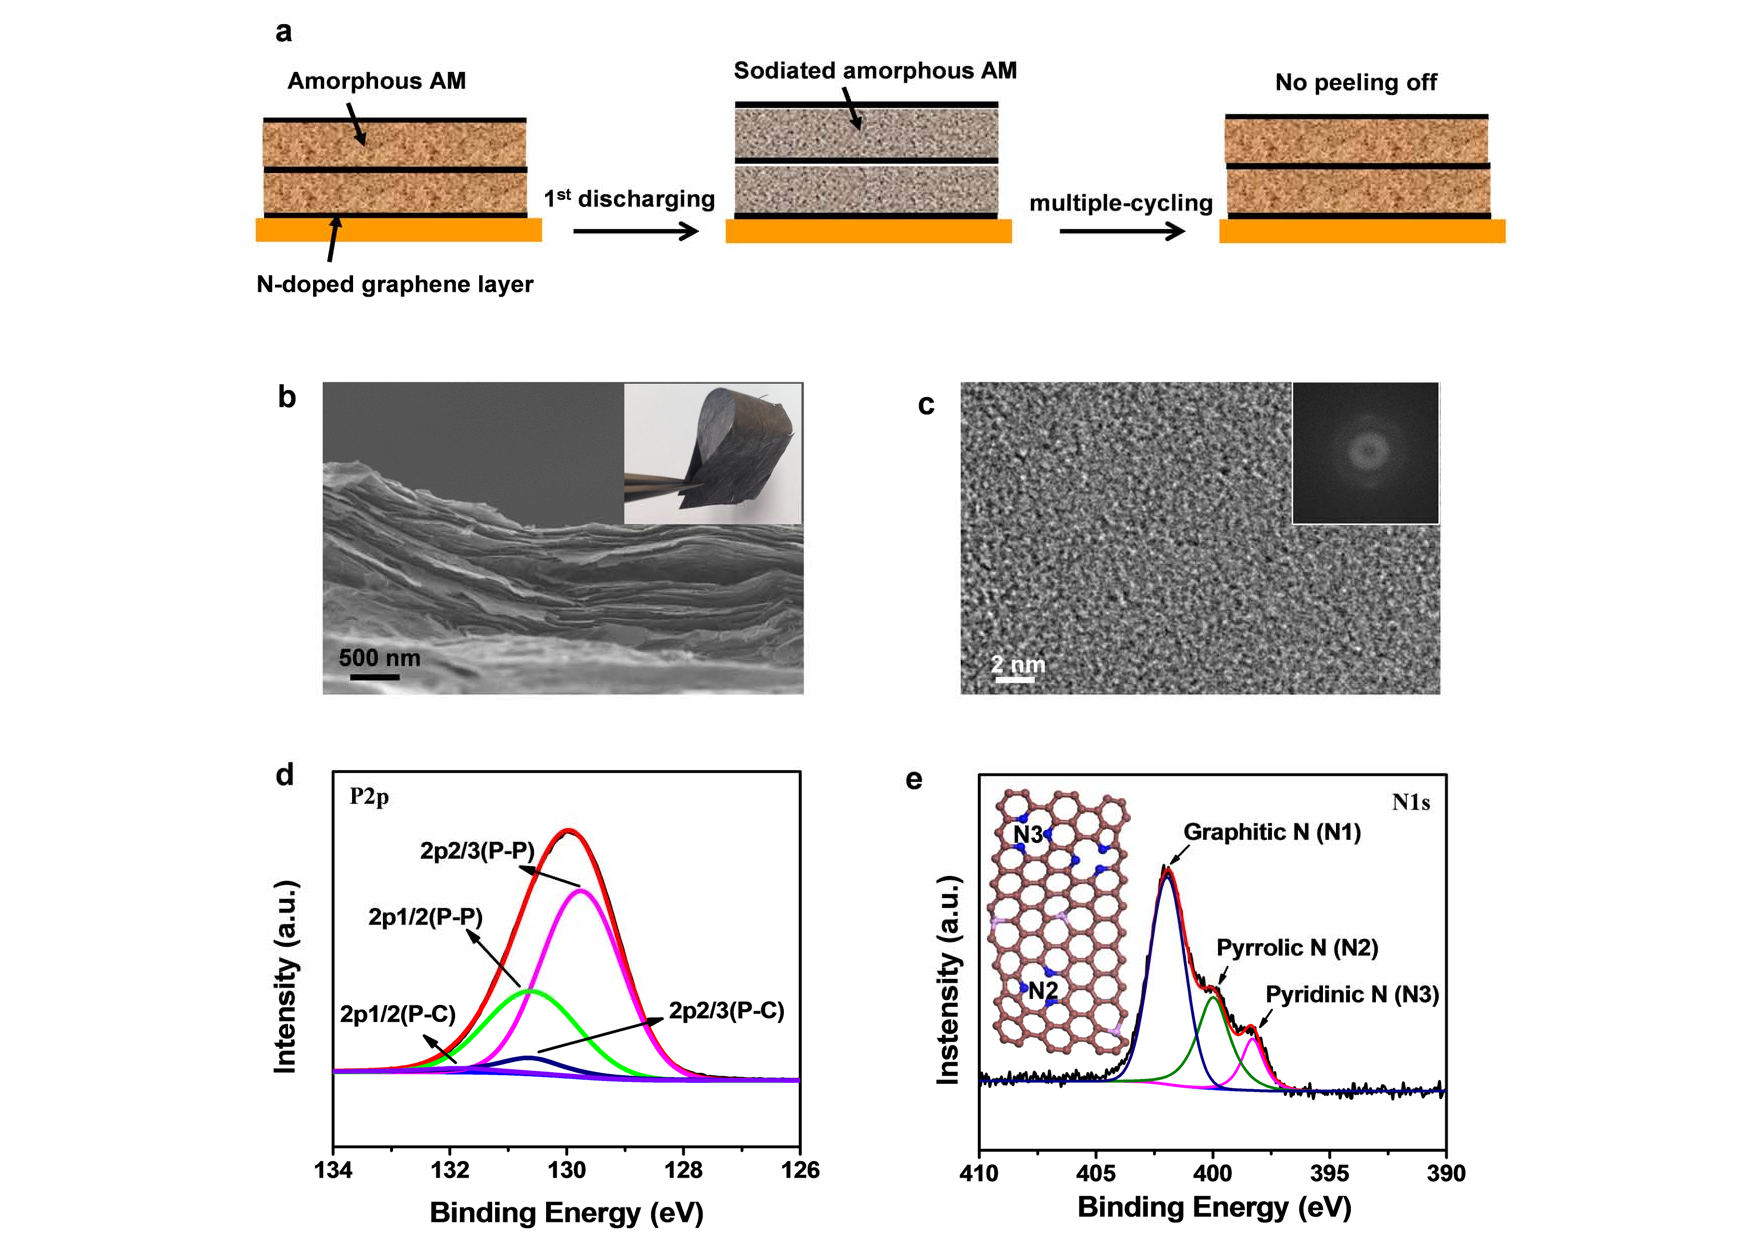
\includegraphics[width=320pt, angle=-90]{figures/figure4_1}
\caption[Layered structure design]
{(a) Illustrative scheme of the designed layered anode structure. (b) SEM image of the cross section of a P@GN paper, the inset shows its paperlike appearance. (c) HRTEM image and the corresponding FFT pattern of the P@GN portion confirming its amorphous structure. d-e) P2p and N1s XPS spectra of P@GN. N2 and N3 represent pyrrolic N and pyridinic N, respectively. 
\label{fig:4_1}}
\end{figure}

To obtain a stable P-based Na-ion battery anode having high capacity retention and rate performance, a flexible hybrid amorphous P-embedded N-doped graphene paper was designed and studied in my work. Unlike the standard methods which assemble the P and C components via any mechanical mixing (milling or grinding), a smarter design should tackle the existing problems, such as electrode chemical stability during sodiation-desodiation and mechanical robustness after hybridization. Therefore, a few-layered N-doped graphene (GN) (Figure \ref{fig:4_s2}) is herein selected as a substrate, whose two-dimensional (2D) nanosheet architecture provides a decent framework ensuring uniform deposition of amorphous P.\cite{Nicolosi2013b,Huang2015b} Several advantages associated with the designed amorphous P@GN hybrids (Figure \ref{fig:4_1}a) prepared by the developed so-called “phase-transformation” route are:\\
(1) Compared with crystalline P (Figure \ref{fig:4_s3}), amorphous P is more stable because of its relatively small volume change.\cite{Qian2013b,Kim2013c} Through the uniform confinement of the amorphous P within GN frameworks, the flexible GN can effectively buffer the volume change. This effectively prevents the electrode fracture and ensures the improvement of the battery capacity retention during electrochemical cycling;\\
(2) The possibly formed robust P-C bonds between P and GN layers anchor both components, serving like several elastic “springs” between them; this also helps to further enhance the stability of the anode;\\
(3) The GN nanosheets provide high conductivity electron transport networks and robust mechanical backbones, so that amorphous P could be very electrochemically active. In addition, the high tenacity of GN is useful to accommodate the volumetric expansion of P without mechanical damage or peeling off effects. Furthermore, N-doped graphene also contributes with a certain capacity to the SIBs and brings the fast sodium ion transport according to the DFT calculations.
Thus in this Chapter, I show that the above-mentioned three key features of the amorphous P@GN structure endows the large-volume-change anode with a superb capacity retention (>85\% over 350 cycles), outstanding cycle stability (0.002\% decay per cycle from 2nd to 350th cycle), and excellent rate capability (809 mAh/g at 1500 mA/g). Most importantly, state-of-the-art {\em in situ} probing experiments in HRTEM and supporting theoretical calculations finally uncover the key advantages of the present design and ensure the future developments of the P-based high-performance SIB anode structures, while getting deep insights into the associated atomistic mechanisms. 

\begin{figure}  
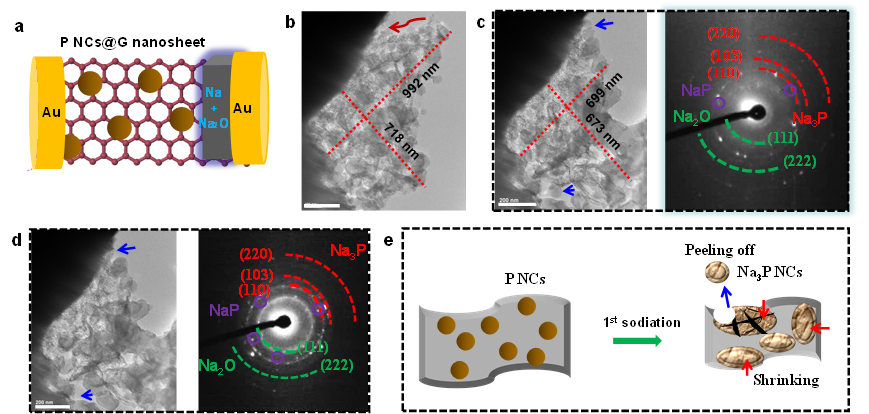
\includegraphics[width=320pt,angle=0]{figures/figure4_s3}
\caption[Layered structure design]
{a) Schematic illustration of an individual P nanocrystals@G (P NCs@G) nanosheet prototype sodium battery device fabricated under {\em in situ} TEM. b) TEM image of the nano-SIB at the initial stage. c-d) Time-dependent TEM images and SAED patterns of sodiated P NCs@G nanosheet upon sodiation at 5 s and 120 s. e) The schematic illustration of the 1st sodiation-desodiation process of P@GN nanosheet. Red arrows indicate the shrinkage, while blue arrows indicate particles peeled off. Scale bars: 200 nm. 
\label{fig:4_s3}}
\end{figure}

\section{Experimental}
%from main text.
Amorphous P@GN paper was prepared by a designed "phase-transformation" route. Bulk red P was heated to form P4 vapors in a sealed ampule, which were adsorbed and deposited within the inter-layers of GN; it changed back into amorphous red P after condensation.\cite{Roth1947b} Thus, a butter-bread-like structure composed of flexible conductive GN layers and thin amorphous red P layers between them was fabricated (Figure \ref{fig:4_1}b). 
%from SI.
Synthesis of P@GN. Graphene oxide (GO) suspension used in this work was prepared via a modified method. 50 mg of graphene oxide was loaded in a ceramic boat in a tube furnace followed by its heat treatment at 600 degrees Celsius for 1.5 hours in a gas mixture of NH3 and Ar (1:2 vol/vol) under a total flow rate of 150 ml/min. Commercial red phosphorus was dispersed in water and put into a Teflon-lined stainless autoclave. The autoclave was heated to 200 degrees Celsius and maintained for 12 h to remove surface oxides. As-prepared N-doped graphene (GN) products were properly mixed together with the pretreated red phosphorus powder, and sealed in an ampule in an inert Ar atmosphere. The sealed reactors were thermally treated at 500 degrees Celsius for 1 hour and then at 280 degrees Celsius for several hrs in the furnace, before natural cooling to room temperature. The final product was washed with CS2, water and methanol, and then dried at 60 degrees.\\

Characterization. TEM images were taken with a 300 kV JEOL 3000F microscope. Samples were first dispersed in ethanol and then collected using carbon-film-covered copper grids. To avoid possible electron beam effects (such as radiolysis or sputtering damage of both Na-containing species and graphene lattice) the beam intensity was minimized. Scanning electron microscopy (SEM) images were recorded on a Hitachi S4800 electron microscope operating at 15 kV. XRD patterns were taken on a Philips X Pert PRO MPD X-ray diffractometer operated at 35 kV and 45 mA with Cu Kα radiation. XPS measurements were carried out on an ESCALab220i-XL spectrometer by using a twin-anode Al Ka (1486.6 eV) X-ray source. All the spectra were calibrated to the binding energy of C 1s peak at 284.6 eV. The background pressure was ~3 x 10-7 Pa. Raman spectra were collected on a Horiba Jobin-Yoon T6400 Raman spectrometer.\\
Electrochemical tests: The electrochemical properties of P@GN and P NCs@G samples were studied using a 2032-type coin cell on a Hokudo Denko Charge/Discharge apparatus. The working electrode was prepared by directly pressing a piece of sample onto the Cu mesh current collector. Na metal foil was selected as the reference and counter electrode. The electrolyte was 1 M NaPF6 in ethyl carbonate (EC) and diethyl carbonate (DEC) ($EC : DEC = 1 : 1 vol/vol$). The cells were assembled in a glove box filled with a pure argon gas.\\ 
Construction of individual prototype P@GN (P NCs@G)-based SIB. In situ TEM observations were conducted in a JEOL-3100 FEF equipped with an Omega filter and a {\em Nanofactory Instruments} STM-TEM holder. In order to build up the test cell, an individual P@GN or P NCs@G nanosheets were attached to the fresh-cut flattened Au wire, which was then attached to the piezo-manipulator. A small piece of Na foil was placed to another Au wire as a reference and counter electrode. Before insertion of the holder into the TEM column, a piece of Na foil covered with a Na2O layer was placed on the surface of metal Au tip. Then isolated P@GN or P NCs@G samples were chosen for direct electrochemical tests. Under the following delicate piezo-driven TEM mechanical manipulations the two electrodes were connected and the probe cell was finally constructed. The sodiation was carried out at a negative bias in the range of -2 V to 0 V with respect to the Na metal.\\
DFT calculations. The first principle calculations were carried out using the Vienna ab initio simulation package (VASP),\cite{Kresse1996} where projected-augmented-wave (PAW) potential was adopted.\cite{Kresse1999} The functional of Perdew, Burke, and Ernzerhof (PBE) and the generalized gradient approximation (GGA)\cite{Perdew1996} were employed in the calculations. We used a $3\times3\times1$ mesh in the irreducible Brillouin zone for structure relaxation and $6\times6\times1$ mesh for self-consisted calculations. In all the calculations the forces were relaxed to the values lower than 0.02 eV per angstrom.

\section{Results and disscussions}

%text above is edited by prof on Nov9. 
%the following part is added on Nov10, which is rephrased by zc on Dec 29.

\begin{figure}  

\includegraphics[width=\textwidth]{figures/figure4_s4}
\caption[TGA curve of P@GN]
{TGA curve of P@GN sample.
\label{fig:4_s4}}
\end{figure}

It is considered that some P-C bonds possibly exist between amorphous P and GN layers which would tightly anchor those layers. Scanning electron microscopy characterization (Figure \ref{fig:4_1}b) illustrates the cross section of the structure of anode, where we can see a lot disordered and flexible layered structures. It is considered that most GN sheets can not be tranfered back to graphite by restacking even under longtime heating or mechanical induced compression.\cite{Huang2015b} From HRTEM image and the corresponding fast Fourier transform (FFT) patterns, crystallography of P is amorphous as depicted in Figure \ref{fig:4_1}c. We are able to observe the disordered nature of P@GN of structure from the diffused rings and the absence of all contrast due to lattice fringes. 

\begin{figure}  
\centering
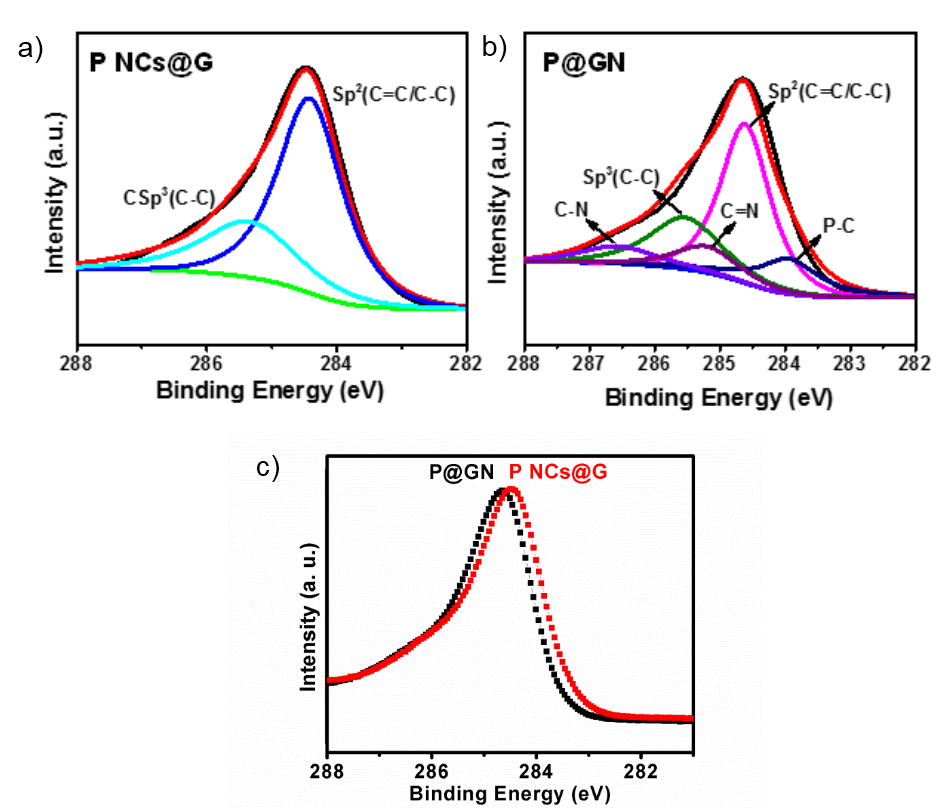
\includegraphics[width=320pt]{figures/figure4_s5}
\caption[C1s XPS spectra comparison]
{a-b) C1s XPS spectra of PNCs@G and P@GN samples. c) Overlay overlay of the two surveys for C1s spectra of the two samples. 
\label{fig:4_s5}}
\end{figure}

The constitution of P in the composite was characteried to be ~66\% by thermogravimetric analysis curve as shown in Figure \ref{fig:4_s4}. In Figure \ref{fig:4_1}d, the P2p X-ray photoelectron spectroscopy (XPS) fit 2p1/2 and 2p3/2 doublets, where two peaks at 129.75 eV (2p3/2) and 130.6 eV (2p1/2) suggest the possible existance of P-C bonding.\cite{Jiao2014b,Niu2014b,Zhang2013b} 

According to theoretical simmulations,\cite{Sun2014b,Claeyssens2009b} among all P-C bonding types -- sp3, sp2 in plane, sp2 at edge, and sp2 in aromatic ring -- the most stable one is the sp2 hybridized P-C bonds in aromatic ring because of bond length in the \pi-p* conjugation plane is the shortest. As the inset image illustrates in Figure \ref{fig:4_1}e, GN would provide sp2 P-C bond at edge and or at aromatic rings. In addition, more evidence from C1s XPS spectra as shown in Figure \ref{fig:4_s5} depicts the possibly existed P-C bonds are observed in P@GN. In order to get clear comparison, P nanocrystlas in pure graphene (this sample name will be short as P NCs@G) sample was also prepared for test. As shown in Figure \ref{fig:4_s5}a, clearly, there is no P-C bond found in P NCs@G. 

As compared with the sample set of P NCs@G, the sp2 carbon atom fraction decreases while sp3 C-C (285.3 eV) bonds prevail in P@GN (Figure \ref{fig:4_s5}b) possibly due to some defects caused by nitrogen doping. Three N-doping types are characterized to exist in P@GN (Figure \ref{fig:4_1}e): graphitic, quaternary N (N1, 401.7 eV), pyrrolic N (N2, 400.2 eV), and pyridinic N (N3, 399.1 eV).\cite{Roth1947b,Wang2012e,Wang2014f,Wang2013i} The N2 and N3 dopants are generally acknowledged to be located at the edges or surface defect sites such as vacancies.\\

\begin{figure}  
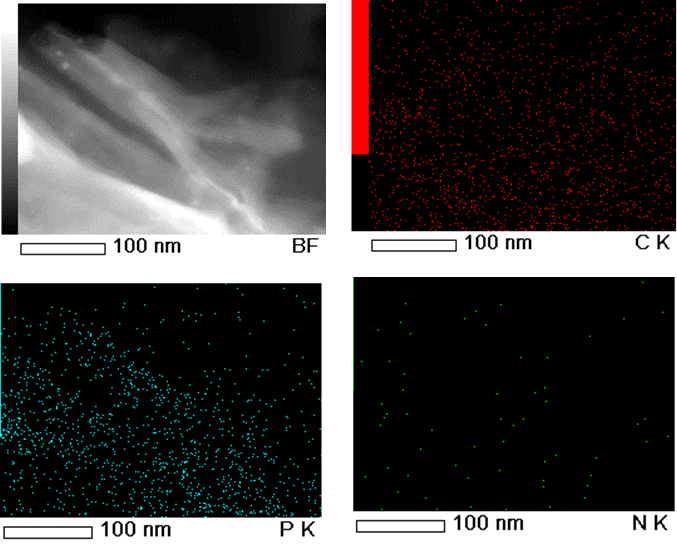
\includegraphics[width=\textwidth]{figures/figure4_s7}
\caption[Elemental maps of P@GN]
{
HAADF-STEM image, and C-, P- and N-elemental maps of a P@GN nanosheet. 
	
\label{fig:4_s7}}
\end{figure}

The specially designed layere structure exhibits revolutionary electrochemical performances. In Figure \ref{fig:4_2}, the battery performances of the P@GN were evaluated by using standard CR2032 coin cells. 

As comparison sample set, red P nanocrystals (NCs) placed on pure graphene (P NCs@G) were also manufactured by grinding of nanoscal red phosphorus and graphene. As shown in Figure \ref{fig:4_2}a, the initial Coulombic efficiency of P@GN is 87\%, higher than a that of 85\% for a reported P@C hybrid electrode.\cite{Li2013c} 
From the 2nd to 120th cycles at 200 mA/g or 350th cycle at 800 mA/g, the Coulombic efficiencies are more than 98\%. A discharge plateau as dipicted in Figure \ref{fig:4_2}b corresponds to an anodic peak starts from 0 V to 0.5 V, implying the formation of \ce{Na3P} with theoretical capacity of 2596 mAh/g. The conversion chemical reaction from P to \ce{Na3P} takes place. 
The chemical reaction process is then eventually proved by {\em in situ} HRTEM experiments which will be discussed in the following paragraphs. In reversed scan, a main anodic peak appears at 0.53 V, which possibly matches to a main sodium ion de-intercalation process of chemical reaction from Na3P to P. However, no clear peaks at any other potentials (for instance 0.63 V assigned to NaP) was found. This indicates that this electrode probably experience a reversible discharging/charging chemical cycling between \ce{Na3P} and P and affords very high capacity because of existence of \ce{Na3P}. \\

\begin{figure}  
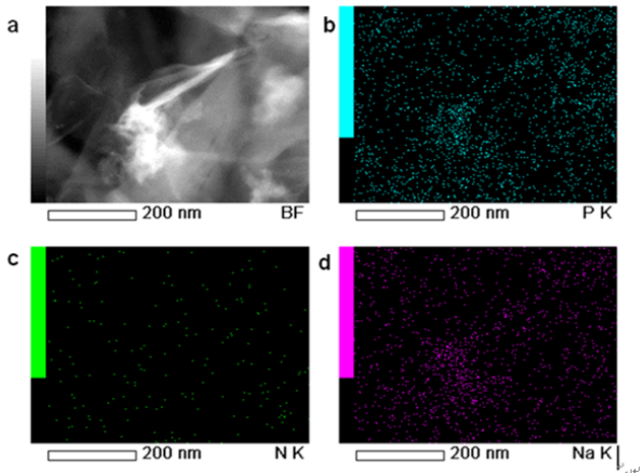
\includegraphics[width=\textwidth]{figures/figure4_s8}
\caption[Elemental maps of P@GN after 150 cycles]
{
The HAADF-STEM image and the corresponding elemental maps of a P@GN nanosheet at the fully desodiated state after 150 cycles.
	
\label{fig:4_s8}}
\end{figure}

Over 350 battery cycles, the capacity retention of P@GN battery is more than 85\%. From the 2nd to 350th cycle at 200 mA/g, the capacity decay is even less than 3\%. 
The excellent capacity retention and stability (about 0.002\% decay per cycle) are among the best cycling stablity performances of all reported P-based anodes to date. 
To reveal the mechanism of the unusual cyclic stablity, the original and after-cycled P@GN electrodes were examined by a high angular annual dark field (HAADF) imagine in scanning TEM (STEM) mode with the EDS mapping as illustrated in Figure \ref{fig:4_2}c, Figure \ref{fig:4_s7} and Figure \ref{fig:4_s8}. 
Obviously, integrity of the battery structure is maintained quite well in the desodiated states after even 120 cycles. 
It is also noted that upon sodiation, distribution of sodium species is very homogeneous over all nanosheet (Figure \ref{fig:4_2}c), this suggests the successful intercalation of sodium ions. 
The reduced volume expansion of P layers are significantly buffered and confined by GN layers, which is the key for refraining failure of anode structural. 
Moreover, P@GN anode material exhibits improved rate capability as compared with P NCs@G material, which are listed in Figure \ref{fig:4_2}d. 
At high current rate (1500 mA/g), the reversible capacity still reaches 809 mAh/g for P@GN. This capacity is twice higher than that of the theoretical capacity of commercial graphite (370 mAh/g) in LIBs. And, of course, these results are far better than those of the P NCs@G (~10 mAh/g at 1500 mA/g). \\
This is especially meaningful for future secondary battery choice. Sodium batteris are expected to be low cost with high capacity. 

%following part is now reprased by zc on Dec 30. 

\begin{figure}  
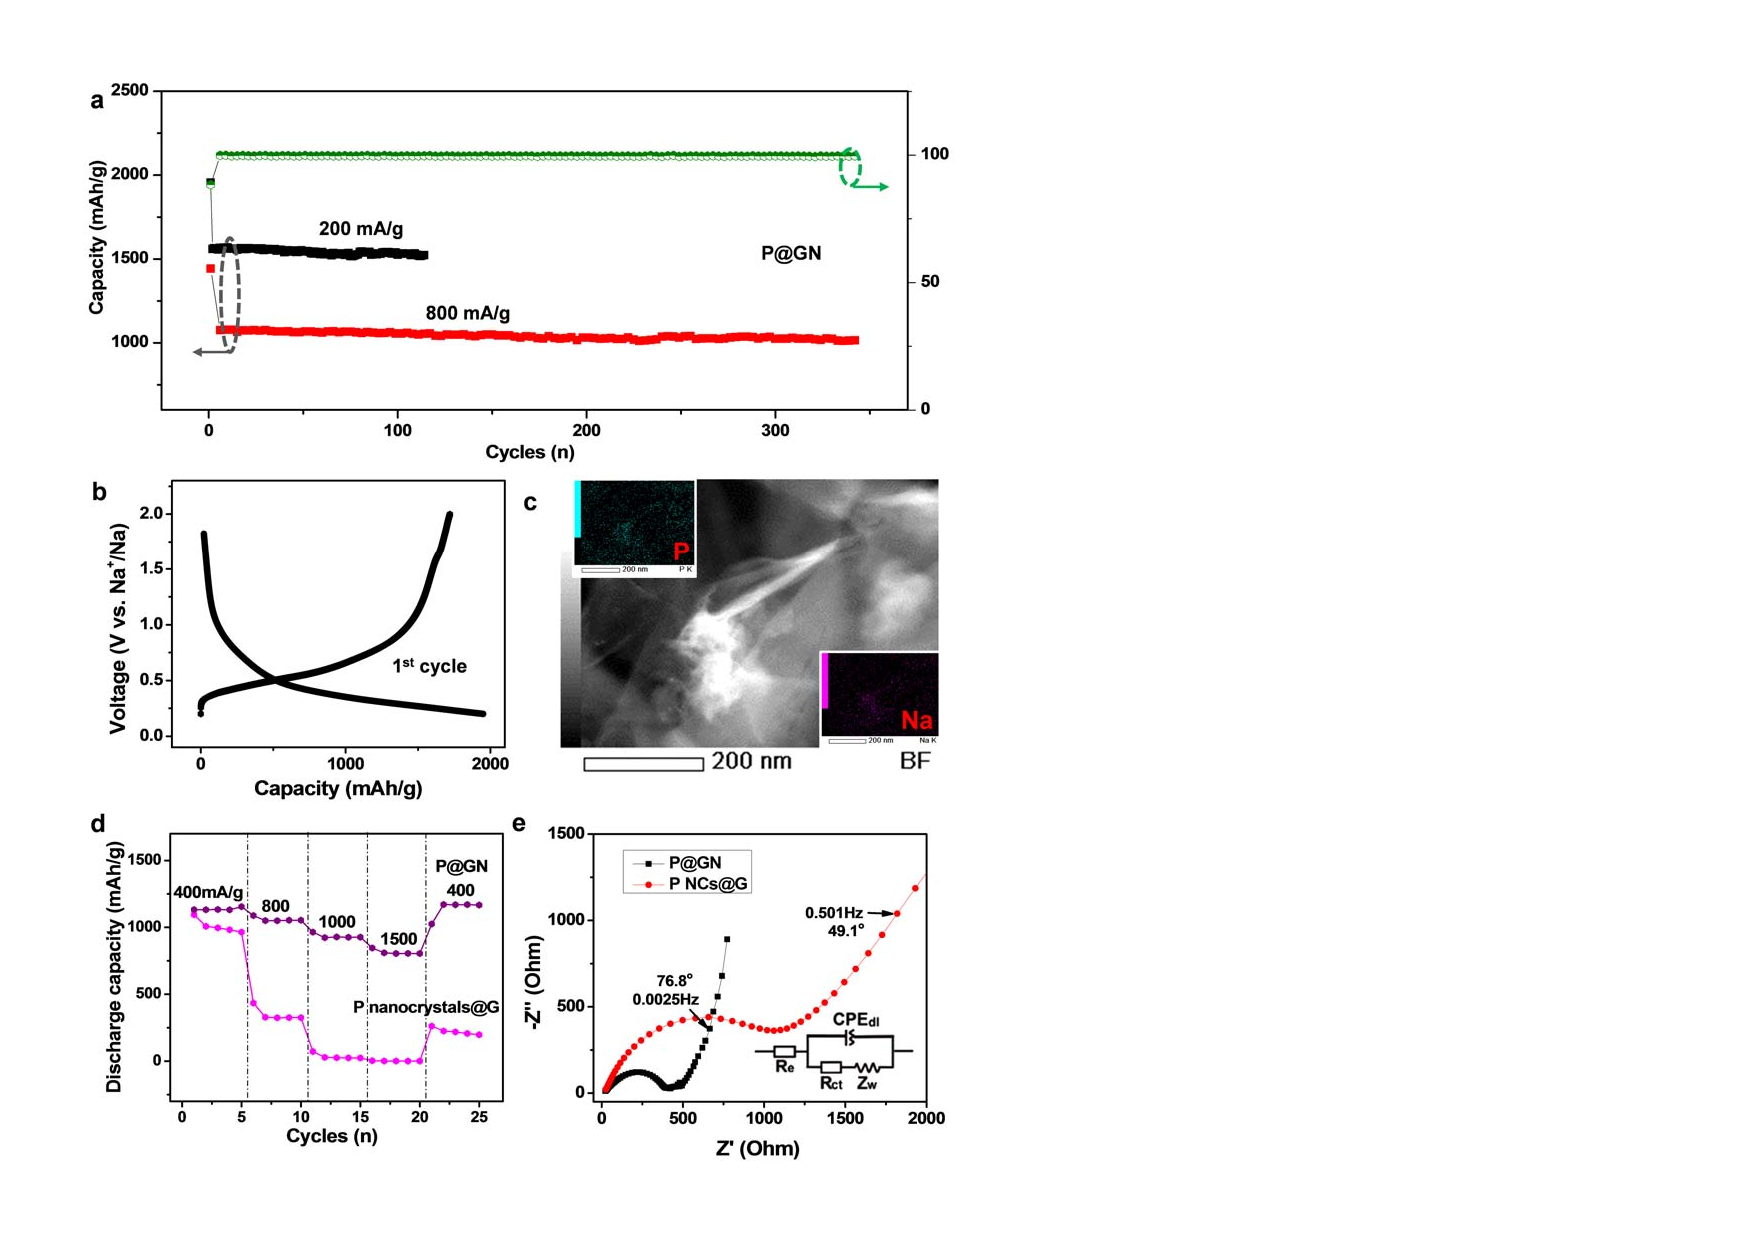
\includegraphics[width=400pt,angle=-90]{figures/figure4_2}
\caption[Performance of P@GN SIB]

(a) Cyclic capacity and Coulombic efficiency of P@GN at 200 mA/g and 800 mA/g. (b) Galvanostatic charge and discharge profile of P@GN anode at 200 mA/g. (c) The HAADF-STEM image and the corresponding EDS maps of a P@GN nanosheet at the desodiated state (after 120 cycles). (d) Rate capabilities of P@GN and P NCs@G. (e) Nyquist plots and equivalent circuit model of P@GN and P NCs@G electrodes after 10 cycles at 0.1 A/g in the discharged state. 
	
\label{fig:4_2}}
\end{figure}

To compare the battery anode kinetics of P@GN and P NCs@G, their electrochemical impedance spectroscopy (EIS) was performed as ploted in Figure \ref{fig:4_2}e. The Nyquist curves demonstrate that a diameter of the semicircle for P@GN anode material in high-medium frequency region is much less than that of P NCs@G electrode. This suggests that P@GN anode possess lower contact and better charge-transfer impedance. Based on the modified Randles equivalent circuit, shown in the inset of Figure \ref{fig:4_2}e, the P@GN anode exhibits a significant lower charge-transfer resistance. Therefore, P@GN holds a high electrical conductance and also provides more stable surfaces such as SEI layer. This leads to the better rate capability and reversible capacity as comparison with P NCs@G. 
In addition, the angle of low-frequency slope for P@GN (76.8 degrees) is steeper than that of P NCs@G (49.1 degrees), indicating higher diffusivity of \ce{Na+} for sodium ion uptake and extraction in P@GN anode due to the steep low-frequency tail.\cite{Sun2014b} \\

\begin{figure}  
\centering
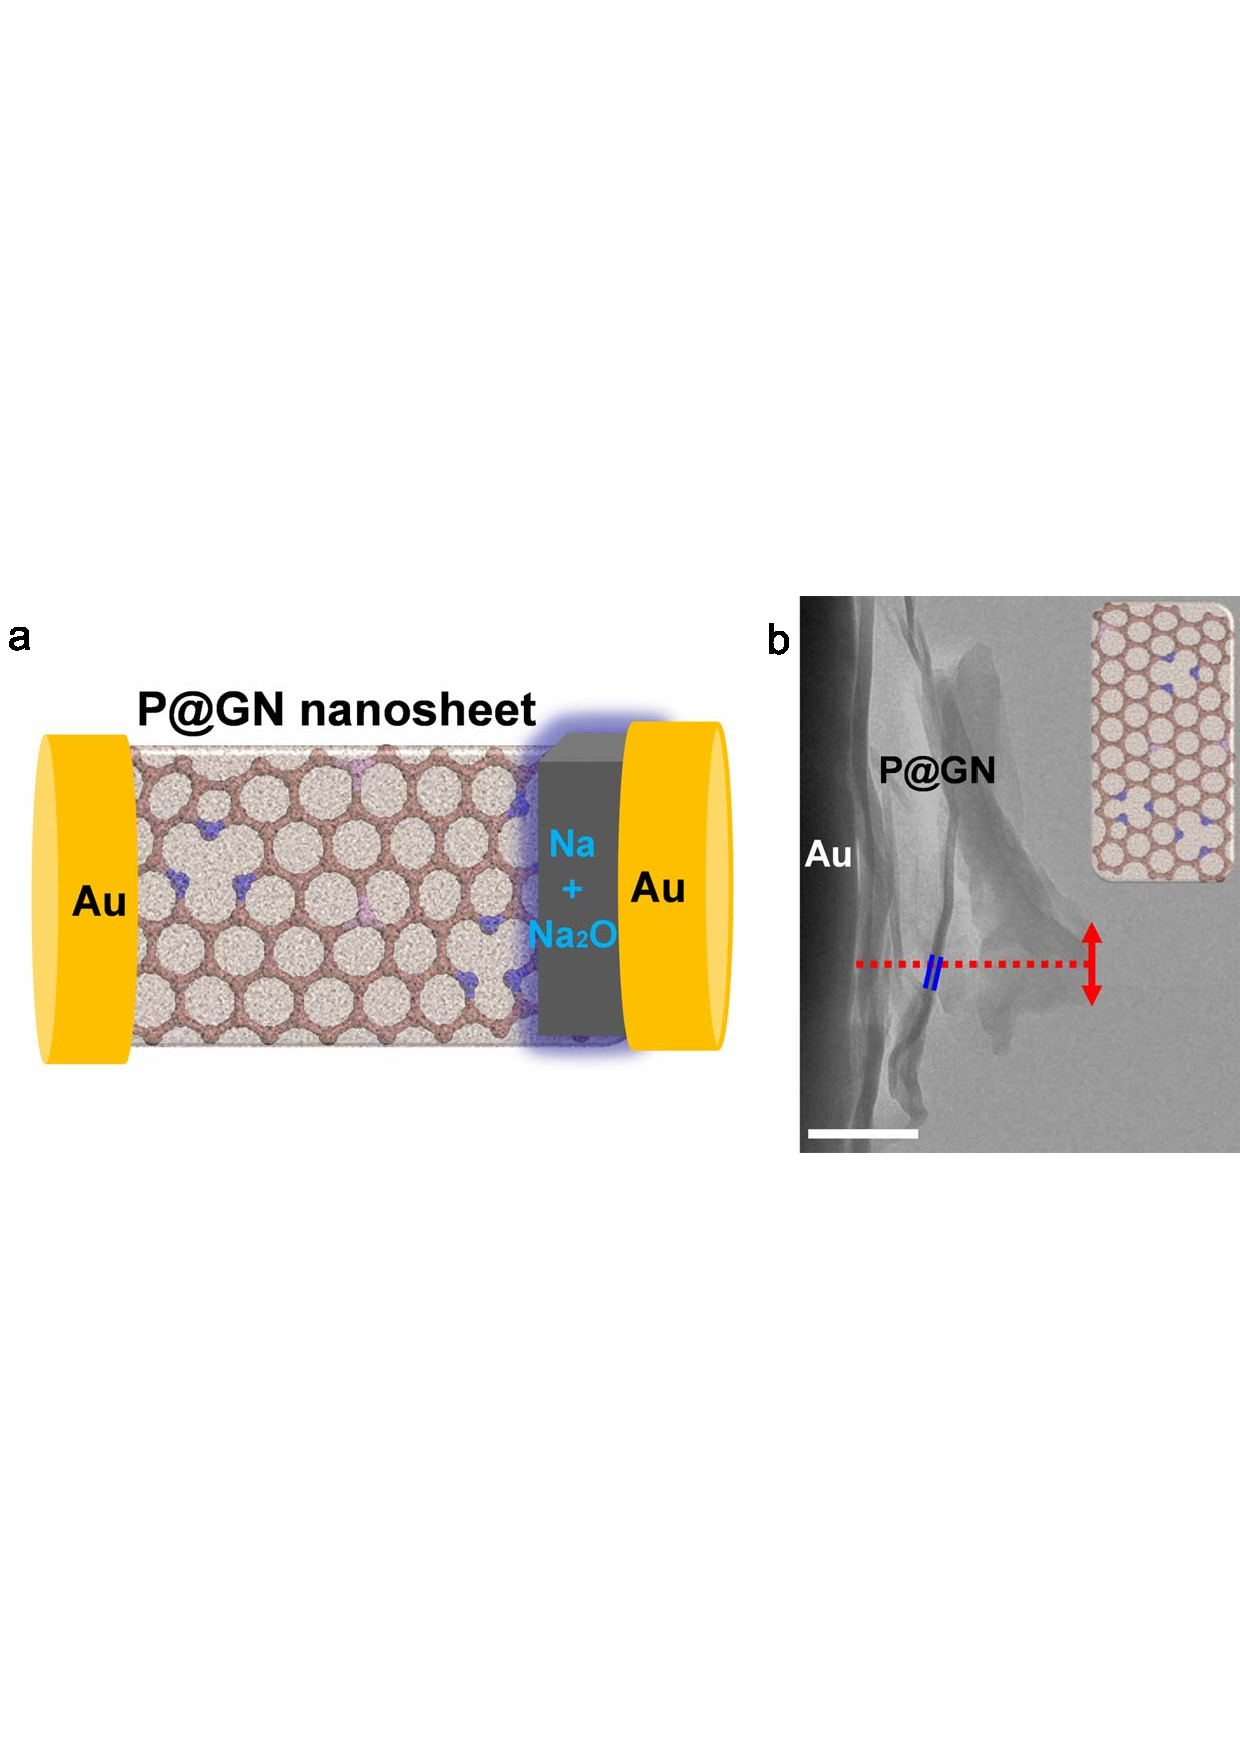
\includegraphics[width=300pt,angle=0]{figures/figure4_3ab}
\caption[{\em in situ} probing on P@GN SIB setup]
{
(a) Schematics of an individual P@GN nanosheet sodium ion battery device test performed by {\em in situ} TEM. 
(b) TEM image of the SIB at initial stage. Scale bars: 100 nm.
\label{fig:4_3ab}}
\end{figure}

It is very important to maintain the structural integrity during cycling to realize stable performance for large capacity and low-cost anode material.\cite{Liu2014a} 
To research mechanism of the anode stability of our ultra-stable decice, I performed an {\em in situ} TEM study of the chemical and structural changes of the as-fabricated anode during electrochemical cycling (Figure \ref{fig:4_3ab}). The {\em in situ} TEM experimental set-up is very similar to some previous reports (Figure \ref{fig:4_3ab}a).\cite{Wang2014f,Wang2012g} 
The setup mainly consists of two parts: the sample is on a gold wire tip, while another gold wire with a small piece of sodium is on the opposite side. Special care is required for sodium loading. Sodium is loaded to the probe (which is on the TEM holder) in glovebox with argon atomosphere. Then the holder was capped with argon. A few seconds before insertion of holder, the cap was removed. 
For transferring process, a very thin layer of \ce{Na2O} was formed on the sodium metal surfaces. The \ce{Na2O} layer serves as natural solid electrolyte for the single nanostructure SIB. Figure \ref{fig:4_3ab}b depicts a TEM image of a freestanding P@GN nanosheet material. 

\begin{figure}  
\centering
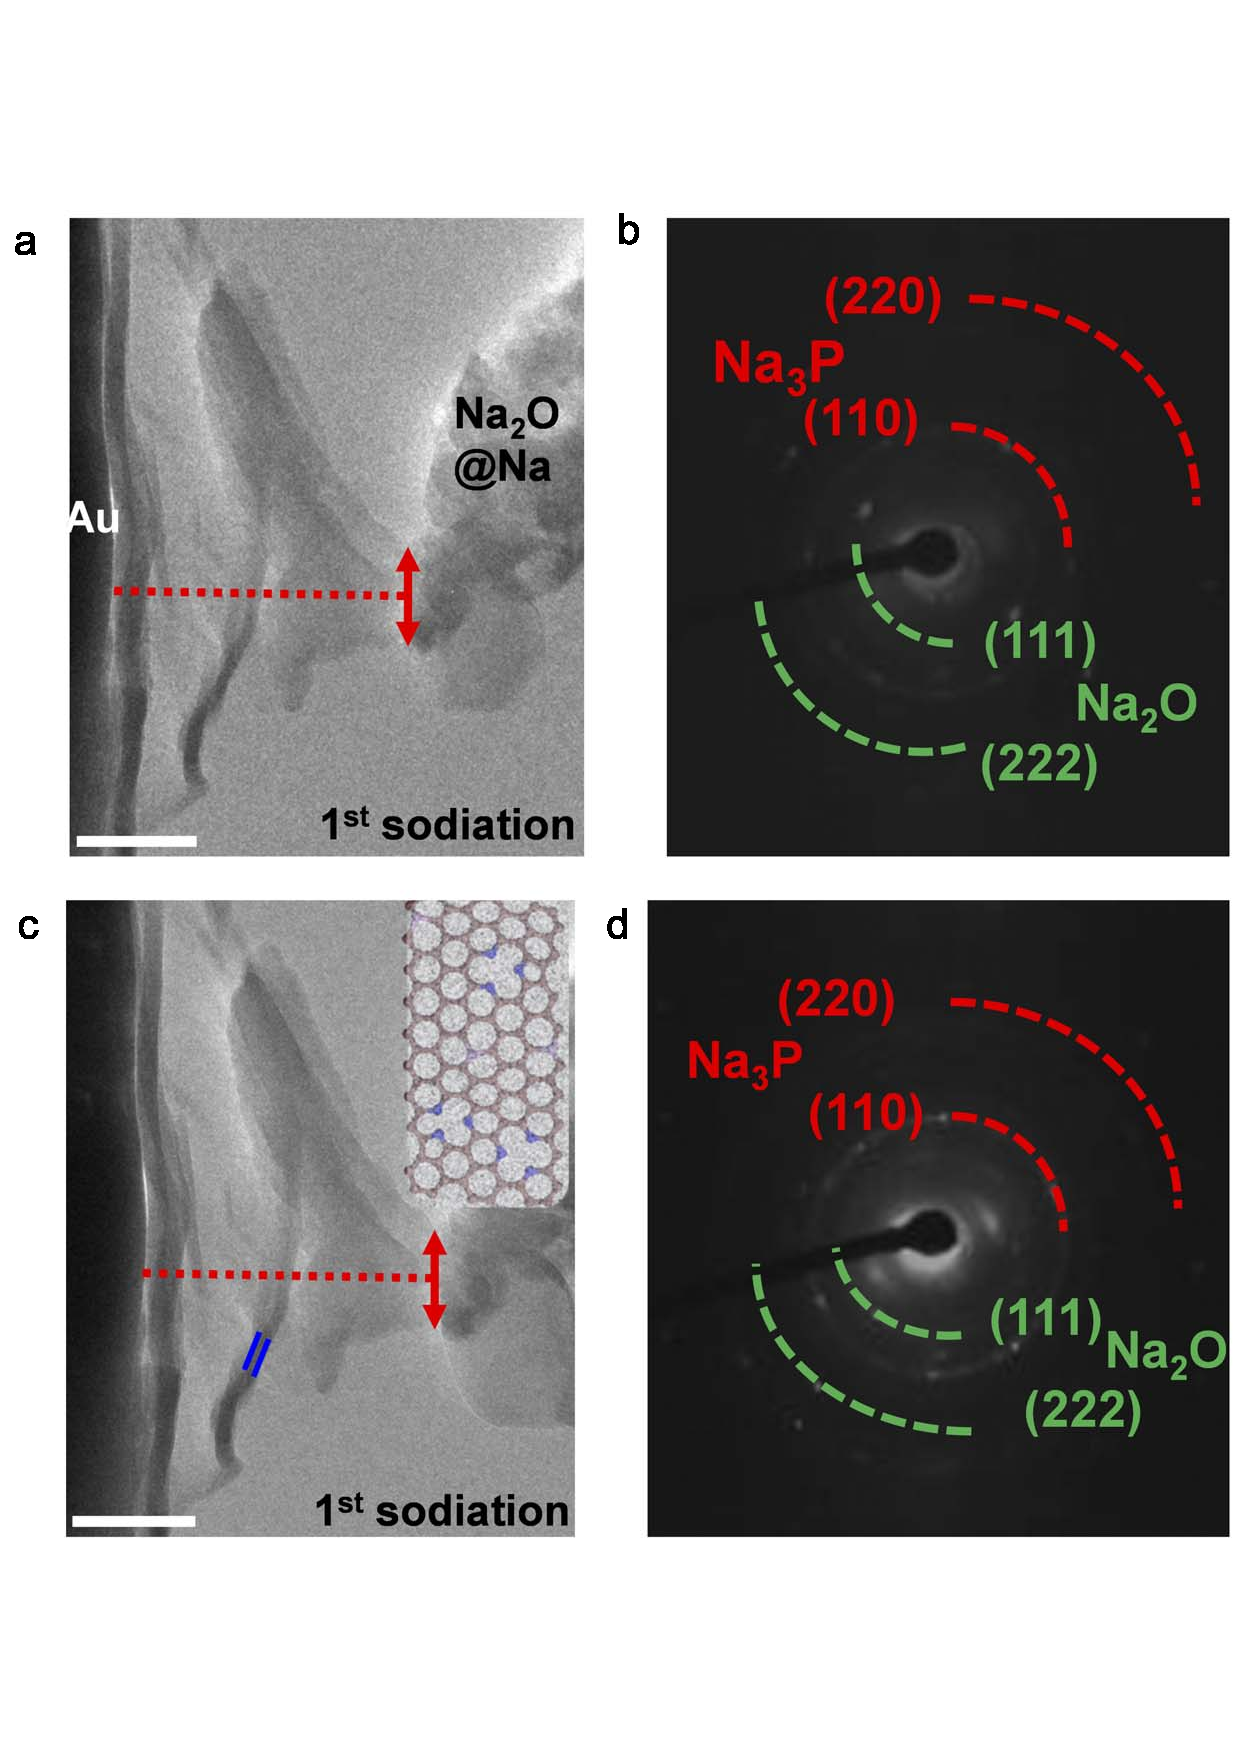
\includegraphics[width=320pt,angle=0]{figures/figure4_3cd}
\caption[{\em in situ} sodiation process of P@GN SIB]
{
 TEM image and SAED pattersn of the {\em in situ} SIB at (a) 15 s and (b) 120 s of sodiation during first discharging. Scale bars: 100 nm.
\label{fig:4_3cd}}
\end{figure}

Figure \ref{fig:4_3cd} present the sodiation process of an individual P@GN anode.
A -2 V potential was applied to P@GN anode with respect to the sodium potential.
The anode material immediately expanded in both longitudinal and transverse directions after the applying of bias, as shown in Figures \ref{fig:4_3cd}. 
After sodiation, the length of nanosheet increased from initial 210 nm to the sodiated 250 nm, and the length of a regional edge enlarged to 83 nm from previous 65 nm. 
The experiment further implies that an effective Na transport along/across the hybrid structure indeed took place. 
It is noted that the expansion rate in the one direction, from 210 nm to 250 nm, becomes less than that for another one, from 65 nm to 83 nm. This might indicate small-sized nanoribbons could process higher electrochemical activities. 
No significant evidence of structural degradation was found even after entire sodiation (Figure \ref{fig:4_3cd}b). This is confirmed by the decent flexibility of GN and amorphous P layer which can effectively buffer large volume expansions during insertion of sodium ions. 
The nanosheet thickness also increased from 10 nm to 14 nm as is marked by blue color in Figures 3b and  3d during discharg process. 
The SAED pattern of the sodiated P@GN (Figure \ref{fig:4_3cd}) reveals the crystallography information of phase changes aftersodiation. 
The main phase of the sodiated anode material is identified to be \ce{Na3P} -- which takes more sodium ions than \ce{NaP} for a single P atom. This result is consistent with the battery test as shown in Figure \ref{fig:4_2}b. 

\begin{figure}  
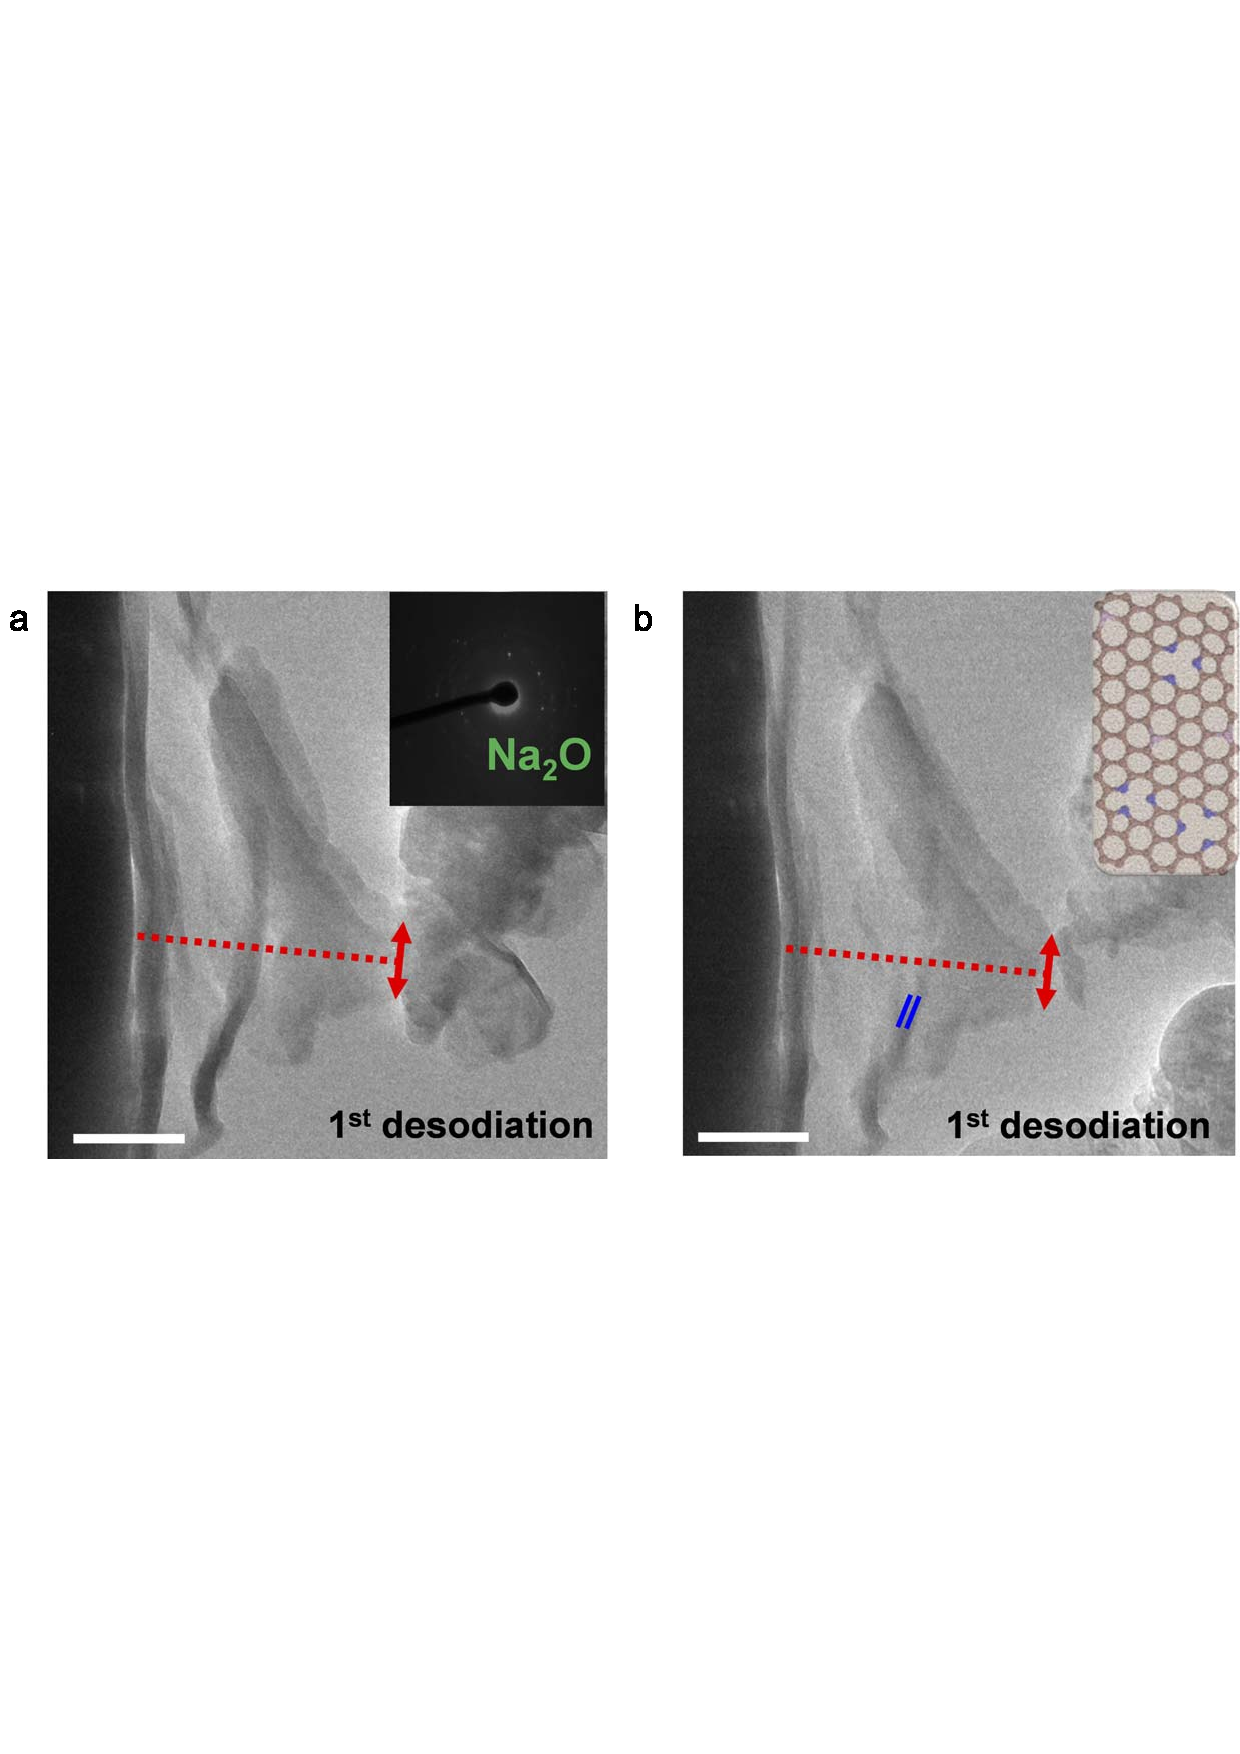
\includegraphics[width=\textwidth,angle=0]{figures/figure4_3ef}
\caption[{\em in situ} desodiation process on P@GN SIB]
{
  (a) 5 s and (b) 120 s of time-dependent TEM images of desodiation during 1st charging. Insets show the corresponding schematic atomic structures. The inset in (a) depicts the corresponding SAED pattern. Scale bars: 100 nm.
\label{fig:4_3ef}}
\end{figure}

%this part is rephrased by zc on Jan 2. 
The desodiation process took place when 2 V bias was applied to the nanostructure. As presented in Figure \ref{fig:4_3ef}, the volume shrinkage became observable along both longitudinal and transverse directions. 
It is observed that desodiated nanosheet after sodium extraction looks quite similar to the initial shape. What's more, the edge segment perfectly kept the pristine state. 
The experiment demonstrates that the designed layerd structure denotes to buffer the anode volume expansion and shrinkage during electrochemical cycling. 
Therefore, the {\em in situ} experiments explain the stable cycling performance as shown in the {\em ex situ} battery measurements (Figure \ref{fig:4_2}b). 
Integrity of P@GN nanosheet is preserved quite well, suggesting that the butter-bread-like structure are effective for relaxing strain and overcoming pulverization caused by volume expansion, and in hence it can be a very promising anode candidate for SIB.\\

The comparison material, indicidual P NCs@G nanosheet, was also build and tested by {\em in situ} microscopy. 
As shown in Figure \ref{fig:4_s3}, during discharging, P nanocrystals expanded immediately. 
The whole P NCs@G nanosheet drastically shrinks instead of expanding upon sodium insertion along all directions, because the sodiated crystals aggregated together and also its size grew larger caused by Ostwald ripening.
Therefore, the large adhesive force between graphene and P NCs compressed all structure into a aggregate form of P NCs. 
Note that the phenomenon is more significant at the edge as compared with the basal plane due to higher electrochemical activities of the edges. 
Moreover, peeling off of active material can also be observed during {\em in situ} TEM process which is marked by blue arrows in Figure \ref{fig:4_s3}c-d. Two particles in the upper part and another nanocrystal in the lower part dissapeared after sodiation. 
The peeling off of active material implies that the P NCs@G experienced significant expansion, which leads to irreversable peeling off, and in hence caused a loss of capacity. 
It is noted that some NaP phases are shown in SAED patterns in Figures \ref{fig:4_3cd}, in the desodiated material. The NaP phases (instead of \ce{Na3P}) implies that only conversion of P into NaP rather than Na3P takes place. We know that \ce{Na3P} holds much higher capacity as 2569 mAh/g than that of NaP, which is only 856 mAh/gh. 
Sodiation of phospherous in P NCs@G sample can be associated with its low electrical conductivity and large crystal size. 
Therfore, the irreversible structural failure and the presence of NaP (instead of \ce{N3P}) undoubtedly limit the performance for P NCs@G. 
The {\em in situ} experiment is consistent with the battery cycling performance and rate properties (Figure \ref{fig:4_2}c). \\

\begin{figure}  
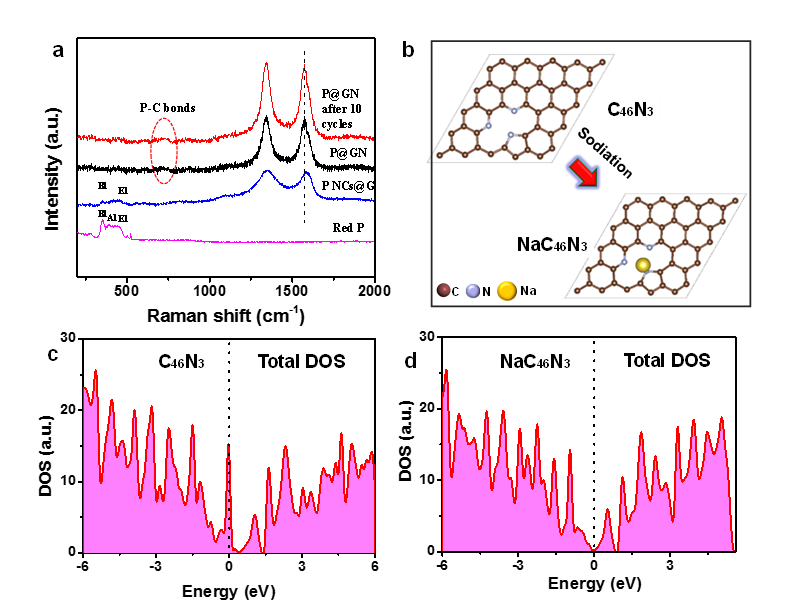
\includegraphics[measuredwidth=\textwidth]{figures/figure4_4}
\caption[Raman spectra and DFT calculations]
{
(a) Raman spectra of red P, P NCs@G, and P@GN before and after sodiation. 
(b) The schematics of the insertion of sodium into a \ce{C46N3} sheet based on DFT calculations. 
(c-d) DOS of \ce{C46N3} and its sodiated product \ce{NaC46N3}.
\label{fig:4_4}}
\end{figure}

It is believed that maintaining amorphous morphology of P during cycling is a key factor for ultrastable battery performance. 
This is confirmed by the Raman spectroscopy presented in Figure \ref{fig:4_4}a. 
Spectrum features of red P between $300~500 cm^{-1}$ can be attributed to P–P stretching bonds of P9 and P7 cages to establish pentagonal tubes in paired layers.

%the rest part... 
Compared with red P material, the present amorphous red phosphorus/graphene hybrid samples (before and after cycling) exhibited no Raman peaks natural for phosphorus; only two typical D- and G- band peaks peculiar to graphene were observed.\cite{Kim2013c} This indicates that a “butter-bread” P@GN paper consisting of amorphous P layers on the GN nanosheets’ was was well preserved during cycling. In addition, Raman spectra of various samples gave an additional evidence of the existence of stable P-C bonds after multiple cycles. As shown in Figure \ref{fig:4_4}a, a broad envelope centered at about $700 cm^-1$ for P@GN (marked as a red circle) is assigned to P-C bond stretching modes. After cycling, a stable P-C bond may exists, as depicted in Figure \ref{fig:4_4}a. The formation of coherent P-C bonds in the P@GN paper affords high capacity and cycling stability during the battery performance. In comparison, no broad peaks exist in P NCs@G and pure red P. Furthermore, compared with P NCs@G, P@GN reveals the G band shifted to a lower wavenumber ($1571 cm^-1$) due to the \pi-p* conjugation, further indicating that the formation of P-C bonds may take place. \\
Finally, DFT calculations were performed to elucidate the role of N-doped graphene on the improvement of electrochemical performances of SIBs. There have been many reports on doped graphenes (GD) utilized as LIB and SIB anode materials.\cite{Yang2011c,Wen2014b,Wang2013h,Wang2012e,Wang2014f} Firstly, we calculated the adsorption energy of a Na ion on different graphene structures. For pristine graphene and graphitic (N1)-doped graphene, this value is positive (e.g. +0.50 eV for G). It demonstrates that both pure and N1-doped graphene make the Na adsorption energetically unfavorable, that is, these two structures deliver no capacity. In contrast, for other doping forms, such as N2-/N3-doping and P-doping, it becomes negative, making them very attractive anode candidates. Herein three types of doped graphene were taken into account; the corresponding Na absorption configurations on the GN surfaces are shown in Figure \ref{fig:4_4}b. Then we obtained their corresponding capacities based on the calculation of the maximum Na concentration. Pure graphene(G) does not have charge transfer, and hence the calculated capacity is idealy 0; while C46N3(GN) present 0.851 e charge transfer, and the calculated capacity is 373.3 mAh/g, which is 1.2 times of the capacity of hard carbon (300 mAh/g) in SIBs, suggesting that N- and P-doped graphenes can contribute to capacity in addition to their positive roles in electron transport. Furthermore, the above-mentioned three kinds of doped graphenes exhibited a relatively larger charge transfer from Na, for example, Na donates 0.853|e| charge to graphene in C46N3. This further suggests that doping sites can have high efficiency to enhance the interaction between Na and graphene surface, leading to ultrafast sodium storage. The high rate capability of the doped graphene was also supported by the density of states calculations (Figures \ref{fig:4_4}c-d). For instance, doping with nitrogen makes C46N3 metallic. Above all, from the theoretical point of view, N-doped graphene is favorable for fast electron/ion transfer, superior rate capability, high capacity, and long cycling life for SIBs.

\section{Conclusions}
In summary, we designed a "phase-transformation" route to fabricate a doped graphene-phosphorous structures with layered morphologies in which very thin amorphous red P layers are formed within flexible and conductive N-doped graphene frameworks. Advantages of such SIB anode designs have been proved experimentally, they are namely: \\
(1) By spreading amorphous P to form a thin P layer on the doped graphene instead of crystalline P nanoparticles, the P@GN anode shows ultrastable efficiency (0.002\% decay per cycle from 2nd to 350th cycle) and excellent rate capability (809 mAh/g at 1500 mA/g); \\
(2) The expected P-C chemical bonds are detected, which firmly anchor GN and P layers; \\
(3) In situ HRTEM experiments on a prototype P@GN-based nanobattery device further verified its ultrastable performance and high capacity of P@GN entirely sustained during sodiation.\\
Finally, DFT calculations reveal that doping sites can enhance the interactions between Na and graphene surface, leading to ultrafast sodium energy storage. Our work demonstrates that the designed flexible amorphous P@N-doped graphene structure prepared from a "phase-transformation" approach can greatly improve the cycling and rate performances for future sodium storage. 




%update: Dec 13 figures added, references pending...
%update: Nov 21 first copy draft

\begin{savequote}[75mm] 
You may say I'm a dreamer, but I'm not the only one. I hope someday you'll join us. And the world will live as one.
\qauthor{John Lennon} 
\end{savequote}

\chapter{Opto-mechano-electrical tripling in ZnO nanowires probed by \emph{In situ} photocurrent spectroscopy in TEM}

\newthought{To find clues} for flexible optoelectronics, light, force and electrons are all important factors to be considered. Photocurrent spectroscopy of individual free-standing ZnO nanowires inside a high-resolution transmission electron microscope (TEM) is reported. By using specially designed optical in situ TEM system capable of scanning tunneling microscopy (STM) probing paired with light illumination, opto-mechano-electrical tripling phenomenon in ZnO nanowires is demonstrated. Splitting of photocurrent spectra at around 3.3 eV under {\em in situ} TEM bending of ZnO nanowires directly corresponds to nanowire deformation and appearance of expanded and compressed nanowire sides. Theoretical simulation of a bent ZnO nanowire has an excellent agreement with the experimental data. The splitting effect could be explained by a change in the valence band structure of ZnO nanowires due to a lattice strain. The strain-induced splitting provides important clues for future flexible piezo-phototronics. 

\section{Introduction}

The current and future progress in transferring large blocks of information at ultra-high speed with marginally low power consumption relies on using photons in optical waveguides instead of electrons in copper wires. However, the social communities are still not completely satisfied with rather small capacities, low speeds, high power consumption and high complexity in integrations of information transfer pathways on rigid or flexible substrates.\cite{C.2009, T.2004, D.2004}
To achieve effective integrations with multi-functionalities, the sizes of light sources for modulators, resonators, light guides, photo-detectors, strain sensors and accelerometers etc. in Micro-Opto-Electro-Mechanical Systems (MOEMS) are expected to reach hundreds of nanometers.\cite{E.2007} However, decreasing size does straightforwardly lead to the optoelectronic device performance enhancement. To catch up with the presently well-established electronics the light-matter interactions should be thoroughly studied and understood both by theoretical simulations and experiments due to the key difference between electrons and photons; the latter exhibit wavelengths down to hundreds of nanometers (UV-visible) and up to ~ 1550 nm (the range which is widely used in fiber communication technologies). However, conventional approaches can hardly detect, operate and modify optoelectronic behaviors of a nanomaterial in real time and at high spatial resolution. 

\begin{figure}  
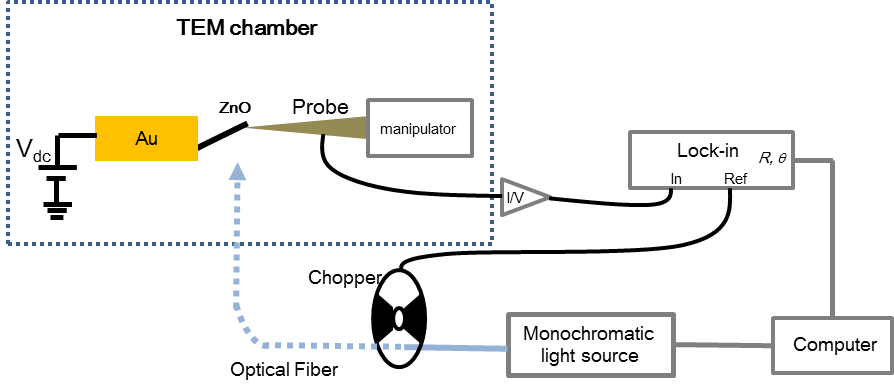
\includegraphics[width=\textwidth]{figures/figure5_1}
\caption[Experimental setup for ZnO.]{Scheme of experimental configuration inside and outside of a high-resolution TEM.
\label{fig:5_1}}
\end{figure}

Moreover, flexible and stretchable optoelectronics attracts general attentions in recent years. Nanowire, as one of scientists’ favorite building blocks for flexible optoelectronics has not been yet carefully studied as a single free-standing physical object. Zinc oxide (ZnO) nanowire is one of the most promising materials for opto-mechano-electrical applications due to its excellent piezo-phototronic properties.\cite{L.2011a,L.2010,D.2015,L.2010a} However, previous reports on flexible nanowire photodiode detectors were performed on materials placed on substrates.\cite{G.2015,H.2014,G.2014} Clearly, choosing a proper substrate is always an essential step in flexible optoelectronics; hence the physical behaviors of a nanostructure are strongly influenced by substrates and spacious metal electrodes. For example, it has been found that the optical absorption coefficient, the band-edge and near-band-edge (NBE) characteristics of ZnO films are all dependent on the substrate quality and subsequent treatments.\cite{R.1997} Therefore, it is essential to characterize mechano-optoelectronic properties of ZnO nanostructures in a free-standing configuration and in high vacuum. For example, Ohno et al. studied photoluminescence and cathodoluminescence (CL) spectra of a diamond crystal in TEM;\cite{S.1995} Yang et al. measured photocurrent values of bent ZnO nanowires in TEM under fixed wavelength light.\cite{E.2012} However, the wide-band-range photocurrent spectroscopy of ZnO nanowires (or any other nanomaterial) has not been studied as yet. 
Herein we report on the photocurrent spectroscopy of individual free-standing ZnO nanowires by means of a special optical-STM-TEM system. It is found that the photocurrent spectra of ZnO nanowires experience a specific splitting, and the shift values perfectly correlate with the bending strains. Under relevant theoretical simulations, the valence band structure was found to change accordingly. The simulations fitted and confirmed the experimental results. 

\section{Experimental}

ZnO nanowires were synthesized by a chemical vapor deposition (CVD) method, as was reported in detail previously.\cite{D.2015} In situ characterizations and manipulations were carried out by an optimized {\em Nanofactory Instruments AB} opto-TEM-STM sample holder with a nanomanipulator and an optical fiber in a 300 kV JEOL-3100FEF (Omega filter) high-resolution microscope. An optical fiber thread inside the side entry holder was connected to the optical system outside of the TEM column. ZnO nanowires were securely attached onto the gold wire stage within the holder tip-frame by using a silver paste. Then, inside TEM, the electrochemically etched sharp tungsten probe was manipulated to contact a pre-selected individual nanowire using the piezo-nanomanipulator, while at the same time, the movable optical fiber was aligned to illuminate the nanowire with a light accordingly. The experimental configuration is schematically shown in Figure \ref{fig:5_1}. By manipulating the tungsten probe, bending of nanowires was precisely controlled. The photocurrent was measured by applying a bias between the two ends of a ZnO nanowire which was directly illuminated by light at a certain wavelength. As a monochromator scanned from 2.5 eV to 4.5 eV, a spectrum of photocurrent vs photon energy could be obtained. Then, by using a lock-in amplifier, photocurrent signal could be rectified according to chopper frequency. 

\begin{figure}  
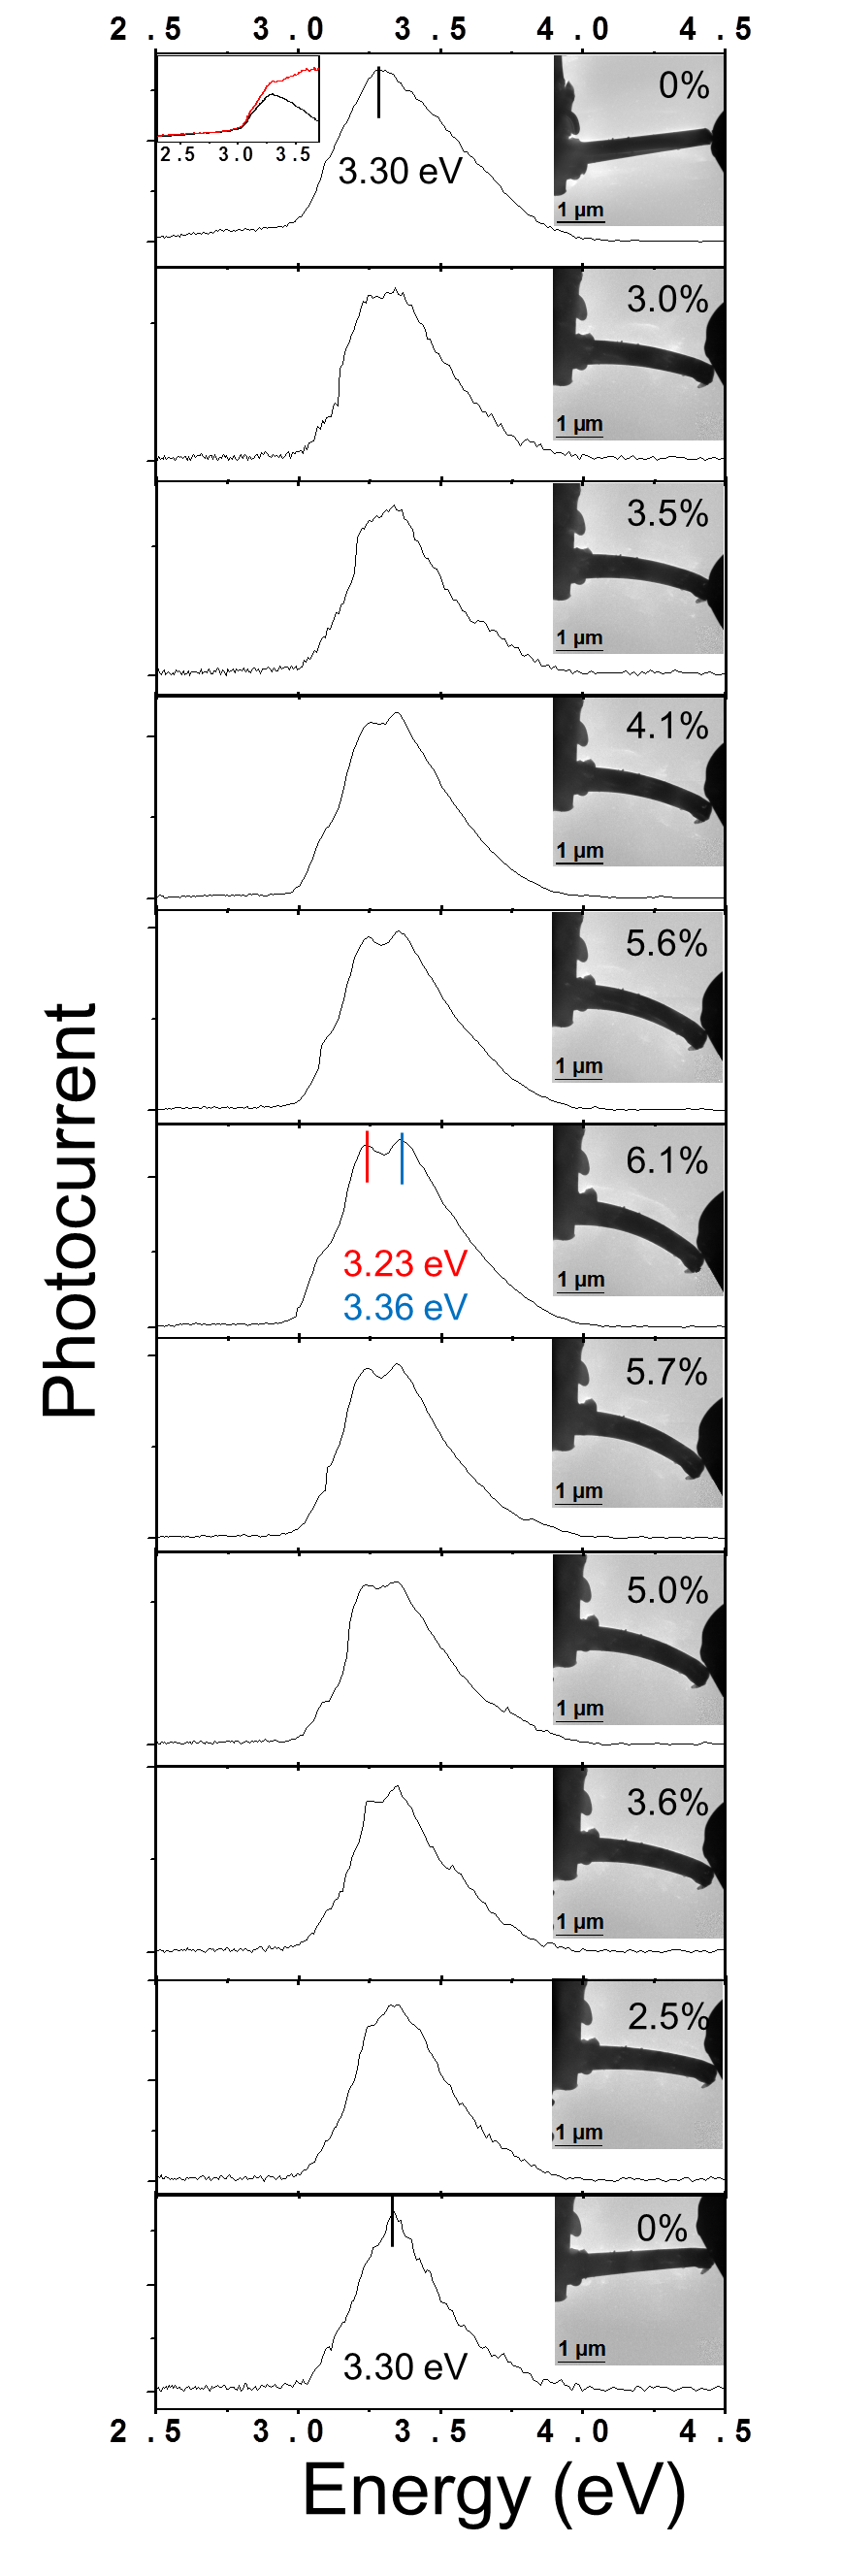
\includegraphics[width=150pt]{figures/figure5_2}
\centering
\caption[Splitting of photocurrent spectroscopy.]{Photocurrent spectra (raw data) measured under bending deformations from 0\% to 6.1\%, and back to 0\%. Red line in the upper left inset of the first panel shows the normalized (to the incident photons) spectrum at the zero strain state (normalized from the measured photocurrents shown as the black line in the inset).
\label{fig:5_2}}
\end{figure}

\section{Results and disscussions}

In Figure \ref{fig:5_2}, a typical experiment on a representative ZnO nanowire is demonstrated. The nanowire was originally straight, as shown in the first panel of Figure \ref{fig:5_2}. The normalized (to the incident photons) spectrum at the zero strain state is displayed in the inset. Due to the large exciton binding energy of ZnO (~60 meV), even at room temperature, a clear exciton absorption peak was observed. By manipulating the probe, the nanowire was forced to bend in the horizontal plane. Photocurrent-wavelength raw data curves in Figure \ref{fig:5_2} demonstrate the regarded splitting phenomenon during photocurrent spectroscopy, which is related to the strain in the bent nanowire. The diameter of the nanowire is 385 nm. The bending ratio, or strain, was determined as follows: $$\epsilon = \frac{r}{R} $$
, where $r$ is a distance from the compressed/expanded side of the nanowire to the middle point of the compressed/expanded region, respectively, $R$ is a radius of curvature of the nanowire. The first manipulation bent the nanowire to a 3.0\% strain, and then gradually to 3.5\%, 4.1\%, 5.55\% and 6.1\%. Finally, the probe was carefully moved backwards, while the strains decreased to 5.66\%, 5.0\%, 3.6\%, 2.5\%, finally giving the initial straight configuration. Before taking a photocurrent spectrum after each manipulation, the electron beam of the microscope was taken off and away from the sample. The inner side of the bent nanowire carries a compressive strain, and its outer side suffers an expansion. The high-resolution image (Figure \ref{fig:5_s2}) clearly demonstrates the nanowire (002) lattice fringes alone c-axis (growth direction) under strain.\cite{zhang2015opto} The lattice distance within the compressed nanowire edge is 0.243 nm, which is smaller than the usual value of 0.260 nm.\cite{L.2011} The lattice distance becomes gradually larger, away from the compressed edge, up to 0.257 nm. Upon bending, the photocurrent spectra first remain of the similar shape with one broad peak centered at around 3.30 eV. However, once the strain increases further, the originally broad peak splits into two fractions. Under a 3.0\% strain, these two peaks are centered at 3.24 eV and 3.34 eV. Thus the detected red-shift and blue-shift are 0.06 eV and 0.04 eV, respectively. Under the largest strain utilized, 6.1\%, the red-shift increases to about 0.07 eV, and the blue shift to 0.06 eV. The splitting values (the gap between the two peaks) of photocurrent spectra of the bent nanowire were 0.01 eV (3.0\%), 0.09 eV (3.5\%), 0.10 eV (4.1\%), 0.12 eV (5.6\%), 0.13 eV (6.1\%), 0.11 eV (5.7\%), 0.13 eV (5.0\%), 0.10 eV (3.6\%) and 0.08 eV (2.5\%), in sequence. The peak positions are displayed in Figure \ref{fig:5_3}(d) to show the relationship with strain values. It is obvious that there is a clear correlation between the strain and peak position shifts. To better understand such correlation, a theoretical simulation was performed. Measuring photocurrent spectrum is one of the methods to obtain the band gap information. Therefore the researchers typically explain photocurrent phenomena by band gap theories. In our work, ZnO nanowire is a well-structured direct band gap material tested without a substrate and in high vacuum conditions peculiar to a high-resolution TEM. Therefore, it is currently reasonable to assume that changing of the band gap is directly connected with the corresponding energy values of the photocurrent peak and its splitting. Because the contribution of splitting is not the prime one with respect to the overall spectrum broadening, and the total spectra contain a photoresponse affected by some pre-existing defects (not created by bending), the spectrum broadening due to splitting is probably hidden. Another fact is that the fiber efficiency used in our measurement system is rather limited. The transmission efficiency descends significantly at the UV range, at around 400 nm (~ 3.1 eV), this cuts off the intensity of the incident light energy. 

\begin{figure}  
\centering
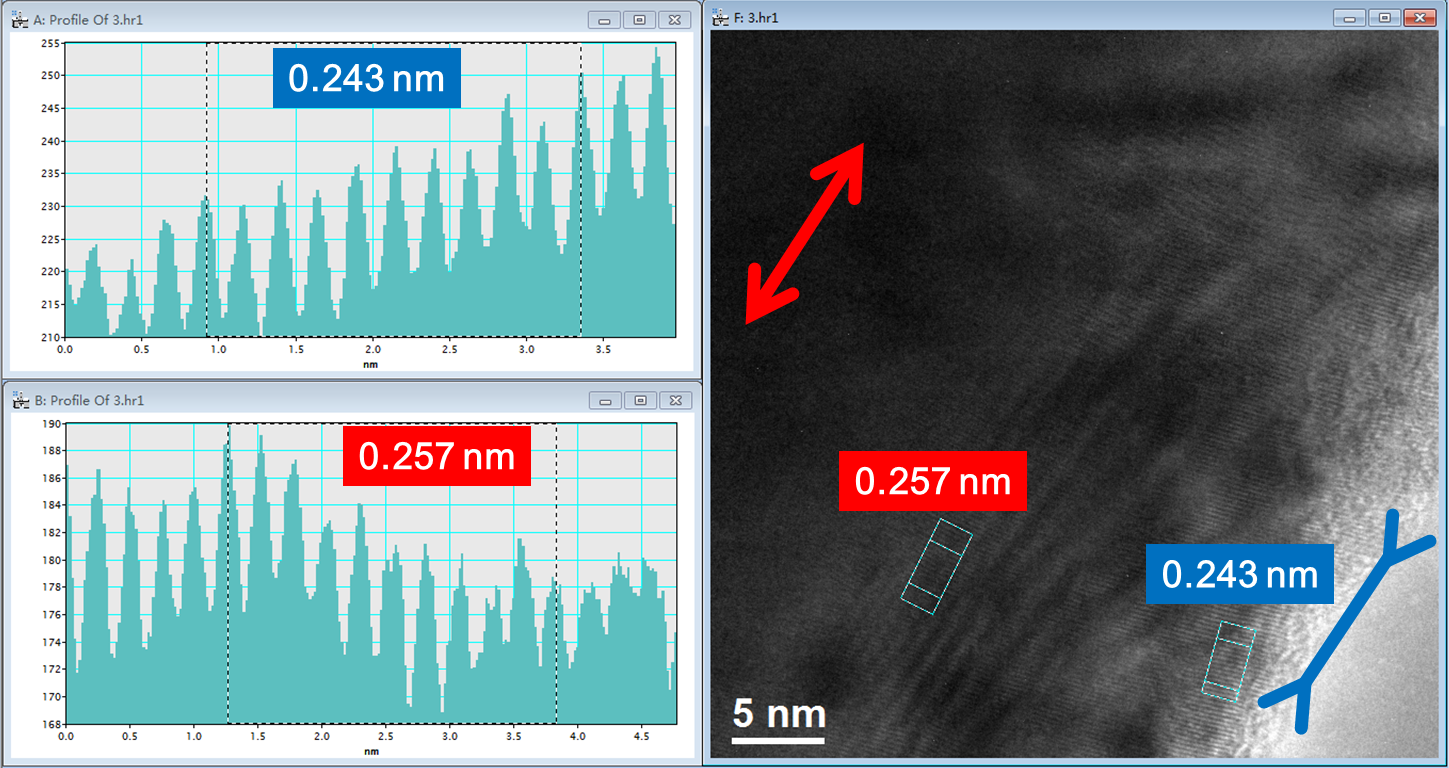
\includegraphics[width=\textwidth]{figures/figure5_s2}
\caption[Localized strain in HRTEM image]{High-resolution TEM image of a bent ZnO nanowire. The (002) lattice fringe separation is 0.243 nm at the very compressed sample edge, and 0.257 nm at the less compressed core. 
\label{fig:5_s2}}
\end{figure}


Theoretical simulation of bent ZnO nanowires was carried out using Density Functional Tight Binding (DFTB) method, implemented in DFTB+ software package.\cite{T.2007} DFTB approach has widely been used for the accurate description of structural, electronic and transport properties of various compounds which contain a large number of atoms in the unit cell (more than 1000). However, because of calculation capability limitations with respect to the number of atoms involved, we simulated a ZnO nanowire with diameter of ~1.5 nm. Parameterization of Zn atom interactions with O atoms has been tested for many bulk Zn-based solids (hcp-Zn, zinc-blende-ZnS and wurtzite-ZnO), ZnO surfaces (clean and with a small amount of adsorbates), and ZnO nanostructures. Such parameterization has provided a reliable description of electronic band structures of ZnO, including reasonable representations of the valence and conduction bands and a band gap of ~ 4.1 eV.\cite{T.2009}

\begin{figure}  
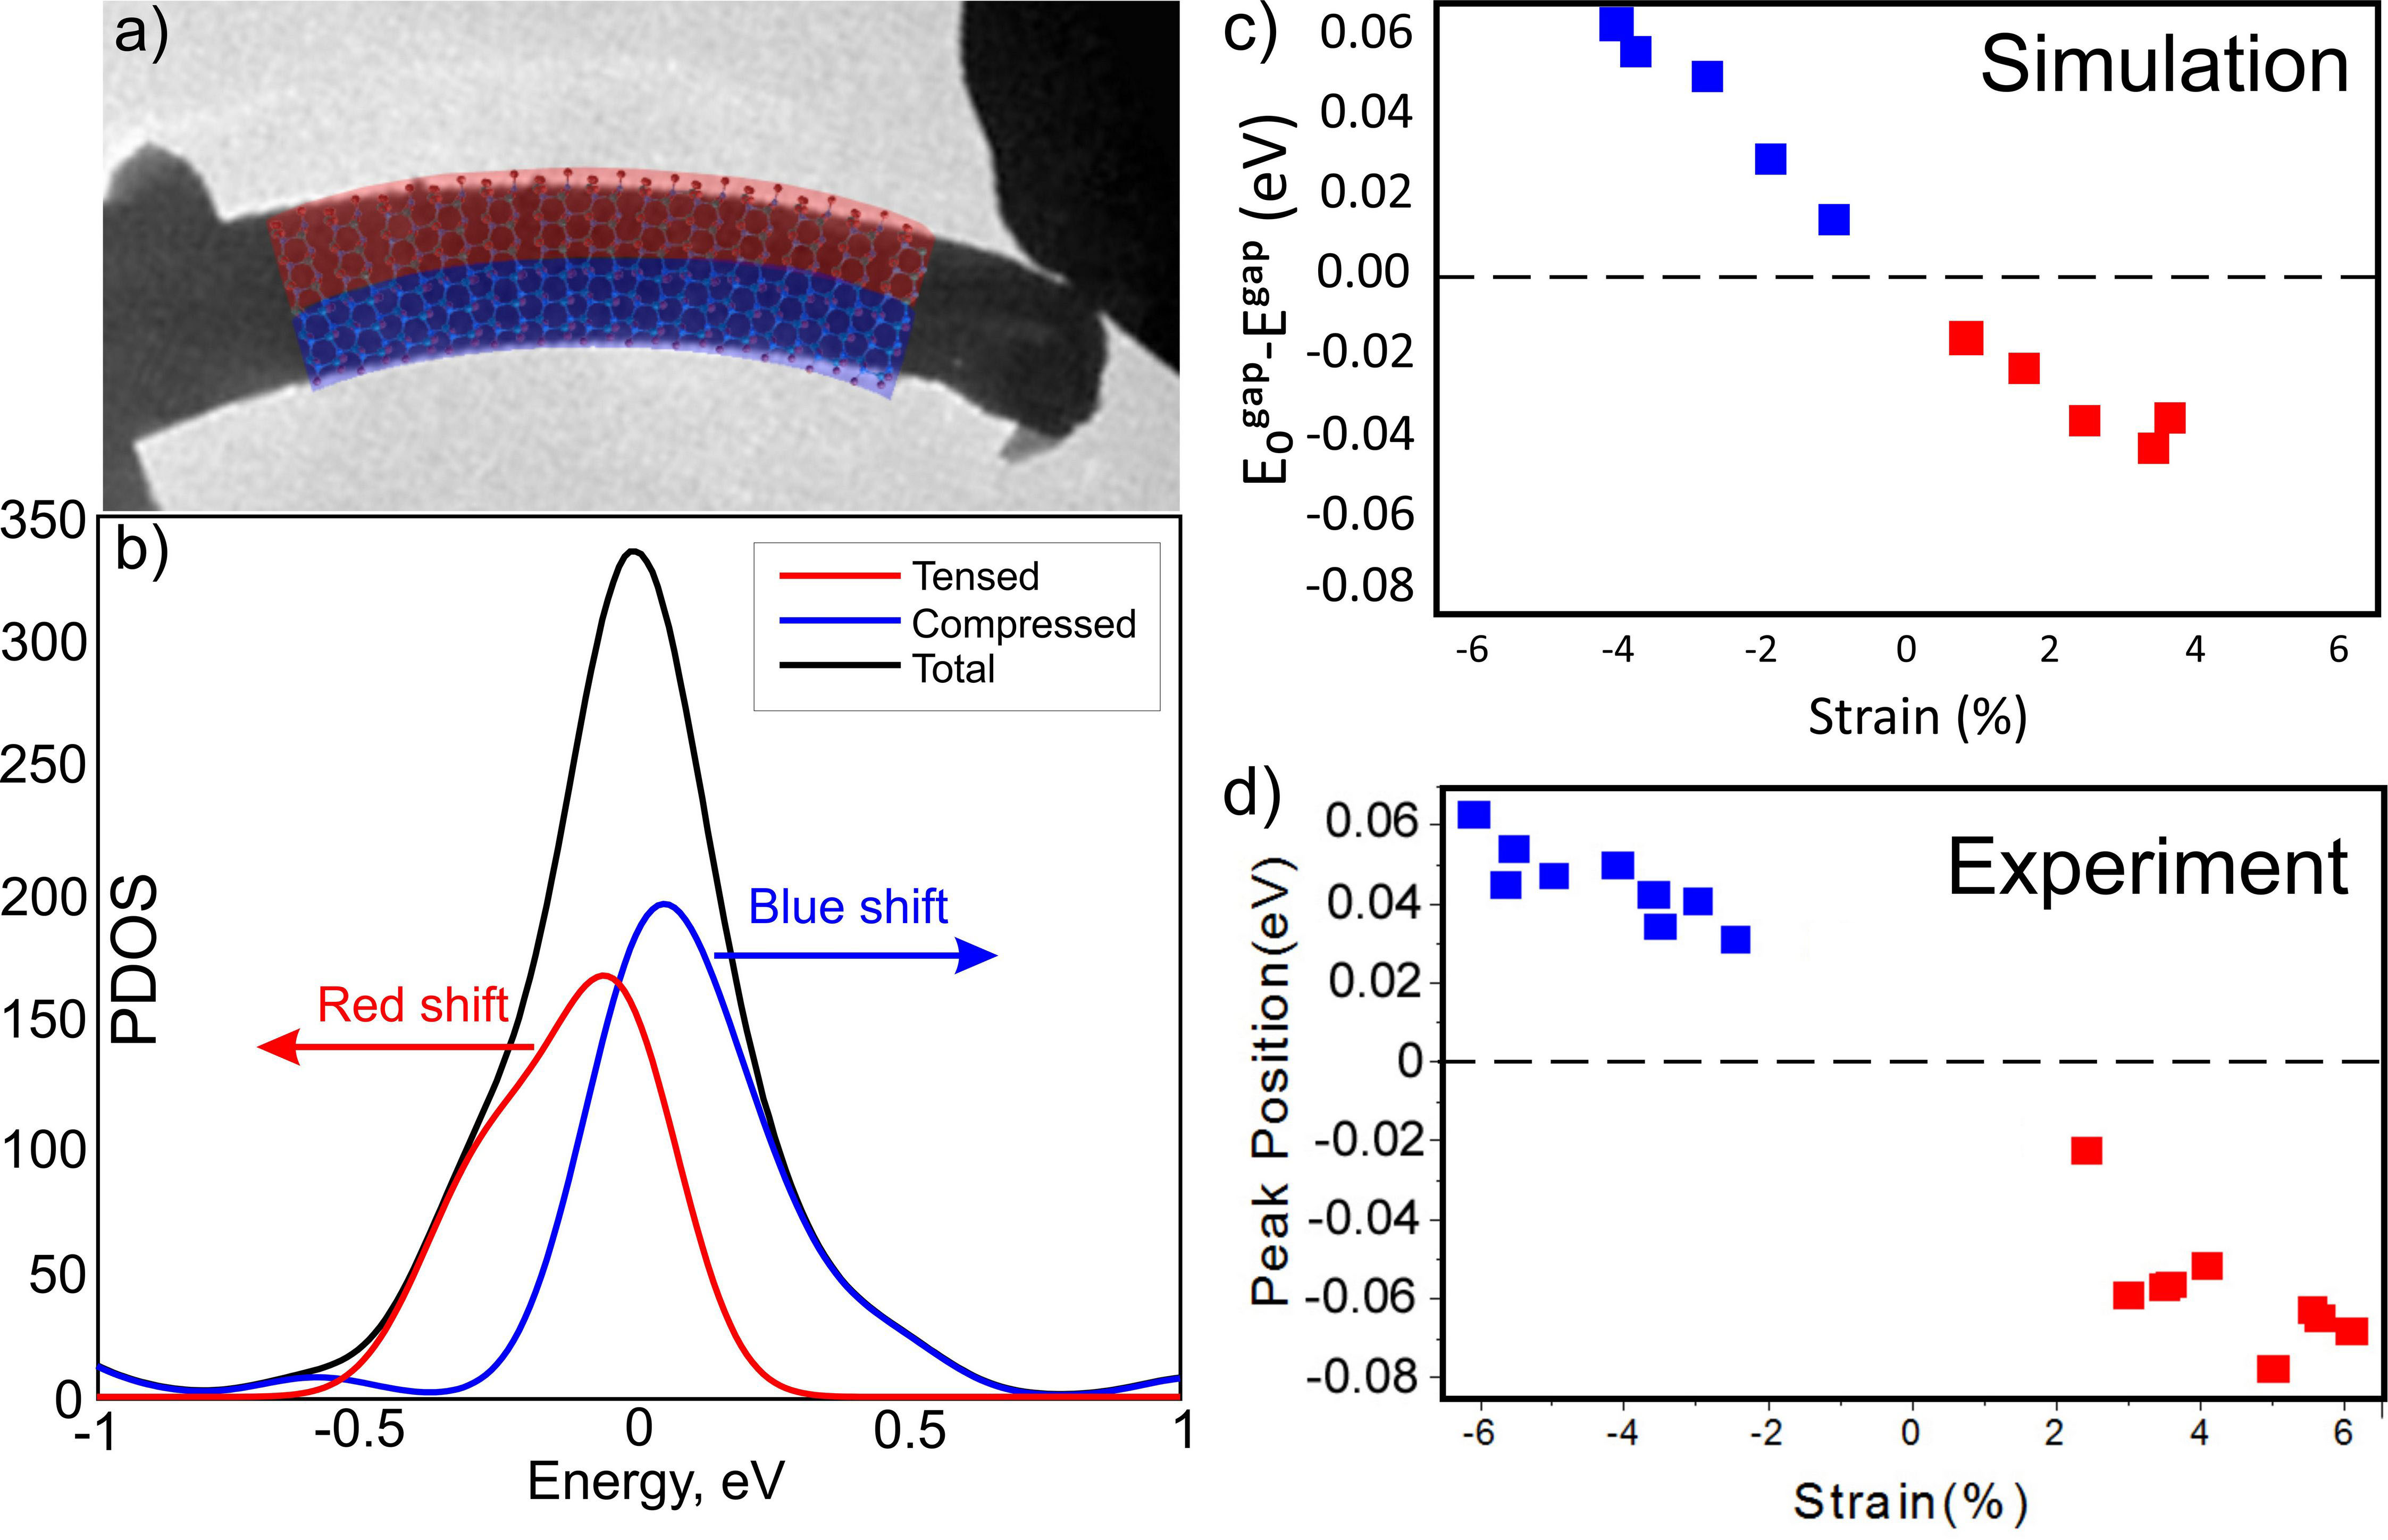
\includegraphics[width=\textwidth]{figures/figure5_3}
\caption[DFTB simulation match experimental result]{(a) Simulated geometry of a bent ZnO nanowire in comparison with the experimental picture. The simulated structure is divided into two parts (marked by red and blue regions) for the calculation of PDOS in expanded and compressed regions. Note that the size of simulation geometry is not the same as for the experimental image. (b) PDOS of expanded (red) and compressed (blue) sides of the deformed ZnO nanowire. Black curve denotes the total DOS for the undeformed nanowire as a whole. Bending strain is about 4\%. (c) Dependence of the ZnO wire band gap on the bending deformation in the frame of the DFTB approach utilized; (d) Dependence of the photocurrent peak position on the bending strain obtained experimentally. Red and blue colors correspond to the expanded and compressed regions of ZnO nanowires, respectively. 
\label{fig:5_3}}
\end{figure}


In the present modeling we simulated bent ZnO nanowires with various degrees of curvature in accord with the experimental deformation values, as shown Figure \ref{fig:5_3}(a). Two sides of the nanowire are marked in red color (expanded side) and blue color (compressive side), respectively. A simulated supercell of ZnO nanowire consisted of 1500 atoms of Zn and O. To avoid the presence of dangling bonds and surface currents over the bent nanowires they were covered by a uniform layer of hydrogen atoms. 
Splitting of the photocurrent peak directly corresponds to the splitting of levels in the valence band at $\Gamma$ point with the corresponding red and blue shifts of the peaked wavelength values under deformation.\cite{D.-P.2012} To calculate the values of splitting partial density of states (PDOS) was computed for the expanded and compressed sides of a nanowire, which is shown in Figure \ref{fig:5_3}(b). During bending, the position of conductive band was not changed; only changes of the valence band were distinguished. In Figure \ref{fig:5_3}(b), the changes in the valence band of the bent ZnO nanowire (having a bending deformation of about 4\%) are presented. PDOS peculiar to the expanded and compressed sides of the ZnO nanowire are depicted in red and blue colors, respectively. Simulation result confirmed that the valence band shifts in a direction of red range of wavelengths, whereas the compression leads to the blue shift, thus in a perfect match with the experimental data. The same calculations were then carried out for ZnO nanowires having various bending deformations (1-4\%). In Figure \ref{fig:5_3}(c) theoretically obtained dependence of the band gap on the bending ratio is shown. The changes in the band gap are directly correlated with the changes in the photocurrent peak positions measured in the experiments, as shown in Figure \ref{fig:5_3}(d). Thus the obtained computation results have an excellent agreement with the experimental data. 
A few reports in regards of bent ZnO nanowires/microwires support our results. Xue et al. probed the strain effects on NBE characterized by CL while studying a curved ZnO nanowire inside a scanning electron microscope (SEM) and found that the emissions had had a relation with the strain ratio.24 Liao et al. also studied CL splitting and shift in bent ZnO microwires in SEM; the authors documented the correlation between the excitation spectra evolution and compressive edges. And it was believed that the valence band splitting had contributed to NBE splitting.\cite{T.2009} In our experiments, the splitting takes place not during CL measurements, which is a process caused by an electron beam to emit light, but during recording of a photocurrent, which is a result of light absorption and electron-hole pairs’ generation. However, both processes share the same deformation conditions which cause the splitting of levels in the valence band at Г point. 


\section{Conclusions}
To sum up, this is a report on opto-mechano-electrical tripling phenomenon under in situ observation and measurements of photocurrents in ZnO nanowires in real time and under the highest spatial resolution natural for a high-resolution TEM instrument. By comparing nicely resolved photocurrent spectra of individual ZnO nanowires under bending deformations splitting of photocurrent spectra is observed. The shifts of photocurrent peaks are directly dependent on the bending strains. The red and blue shifts of ZnO photocurrent peaks under bending are confirmed to be directly related to the splitting of levels in the valence band at $\Gamma$ point. DFTB simulations have an excellent agreement with the experimental data. The discovered splitting effect under specially designed ZnO nanowire photocurrent spectroscopy provides an important information for flexible optoelectronics and piezo-phototronics, for example, for strain tuned wavelength-division multiplexing and MOEMS devices, and for flexible optoelectronics where photocurrent splitting should be evaded. 




%update: Jan 15 fixed grammar according to prof notes
%update: Jan 09-11 prof check
%update: Jan 08 rephrased
%update: Dec 02 figures inserted
%update: Nov 29 citation done, bug fixes
%update: Nov 25 draft

%\begin{savequote}[75mm] 
%I see the world, not as it is, but as I are, or, as I are conditioned to see it.
%\qauthor{Stephen R. Covey} 
%\end{savequote}

\chapter{Statistically Analyzed Photoresponse of CdS Nanowires by \emph{in situ} TEM}

\newthought {To get the missing information for future flexible optoelectronics based on nanoscale building blocks}, as I discussed in Chapter 5, light, force and electrical currents are all important factors to be included into an {\it in siu} probing experiment. 
I demonstrate herein that high resolution TEM coupled with light illumination of a specimen and its electrical/mechanical probing can be applied for the {\em in situ} study of initiated photocurrents in free-standing individual nanowires. 
The crystallography of numerous individual CdS nanowires is analyzed simultaneously with the photocurrent measurements. 
My research implies that elastically deformed wurtzite CdS nanowires show statistically unchanged values of photo-to-dark current (ON/OFF) ratios. 
It is discovered that the cut-off wavelength possesses red shifts of photocurrent spectrum after nanowire bending. 
It is caused by deformation-induced lattice strain or associated changes in the electronic band structure, which is additionally proved by selected area electron diffraction (SAED) analyses and density functional tight binding (DFTB) calculations. 
The stable ratios of ON/OFF ratios, as well as photocurrent spectroscopy shifts of deformed CdS nanowires are important clues for future flexible optoelectronics and photovoltaics.\\

\begin{figure}  [ht]
\centering
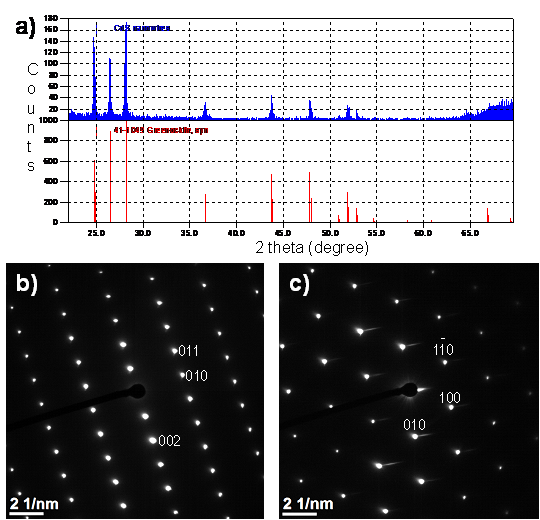
\includegraphics[width=0.8\textwidth]{figures/figure6_s1}
\caption[CdS crystallography]
{(a) XRD data of the nanowire sample (upper panel) fits a CdS hexagonal phase, JCPDS Card No. 41-1049 (lower panel). (b,c) Two SAED patterns of a CdS nanowire taken along the [100] and [001] directions, respectively. 
\label{fig:6_s1}}
\end{figure}

\section{Introduction}
As I mentioned in Chapter 1, flexible electronics and optoelectronics have attracted general public attentions in recent years because of the growing requirements for portable electronic devices having high performance and a low manufacturing cost.\cite{Boland2010,Liu2015,Long2012} 
With high surface-to-volume ratios, excellent carrier mobility and chemically decorated surfaces, which can further be modified/functionalized, one-dimensional inorganic semiconducting nanostructures are attractive candidates for lithium-ion batteries,\cite{Wang2015} future flexible displays,\cite{Klauk2008} solar cells,\cite{Zhang2012} supercapacitors,\cite{Li2014} nanogenerators,\cite{Fan2012} sensors,\cite{Zhang2014d} etc. \\
One of the crucial challenges for future applications is the nanostructure electrical and mechanical statistical stability. 
Although usually most reports claim that the nanowire conductivity is stable during mechanical deformations, there have been no deep and direct investigations related to the photoconductivity or photocurrent spectroscopy of free-standing individual nanowires under conditions which allow for the real-time observations of deformation-induced strains. \\
Hence, it is rather unclear how the crystallography changes in deformed nanowires affect their photoresponses. 
It is noteworthy that some materials were found to be unstable during elastic deformations.\cite{Antsov2014}
Herein, I thoroughly consider these issues by performing {\em in situ} HRTEM experiments using the optical TEM holder discussed in Chapter 2. \\

\begin{figure} [t] 
\centering
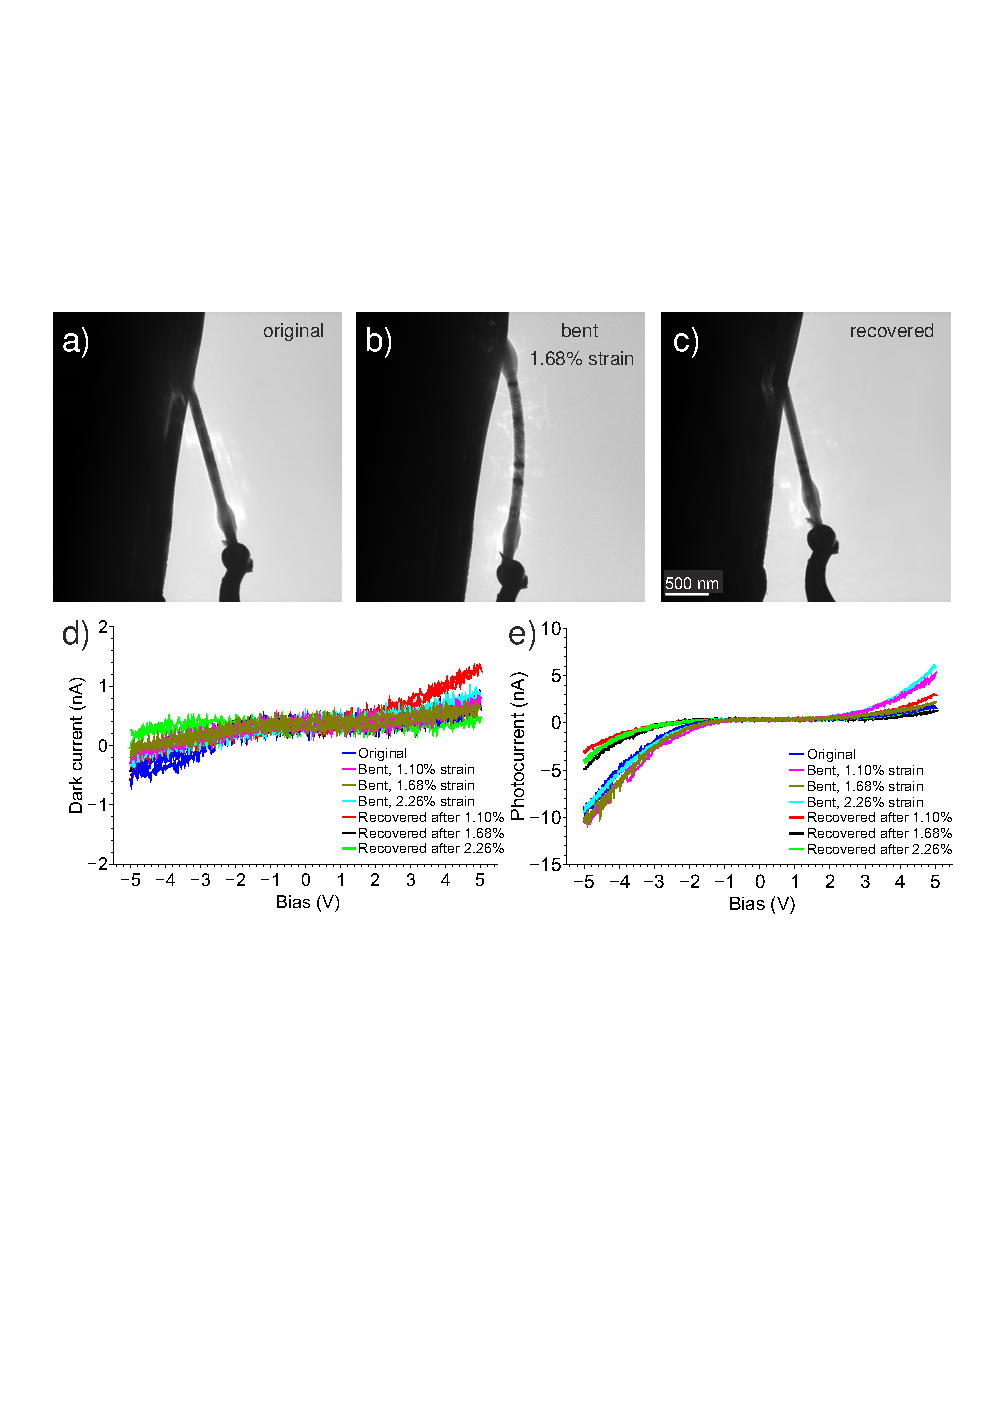
\includegraphics[width=\textwidth]{figures/figure6_2}
\caption[Deformation and I-V measurements]
{Representative TEM images of the original (a), bent (b) and recovered (c) states of an individual CdS nanowire positioned between fixed Au (left hand side) and movable W (right hand side) electrodes; and a summary of dark current (d) and photocurrent (e) measurements at different stages of the bending-recovery process. Calculated strains are marked on the TEM image and I-V plots. 
\label{fig:6_2}}
\end{figure}

I chose cadmium sulfide (CdS), a direct band gap semiconductor for diverse photoelectronic devices, as my testing nanowire material.\cite{Xing2015} 
Using paired probing and microscopy techniques, the electrical currents generated in light-illuminated specimen were measured by source-measuring units. \\
Initial testings revealed an unclear correlation between deformations and current values. 
To exclude the uncertainty introduced by the contact conditions, and to account for the structural diversity of the nanowires, I performed detailed statistical analysis based on numerous sets of experiments. 
Then the photocurrent spectroscopy measurements were performed. The spectroscopy reveals red-shifts for the cut-off wavelength of the nanowires under strain. 
The final part of the work attempts to characterize the strain-induced structural changes using electron diffraction analysis. 
\vfill

\section{Experimental}
CdS nanowires were synthesized via traditional chemical vapor deposition (CVD) method on silicon substrates or graphite plates. The fabrication conditions were reported in my published work.\cite{Zhang2015} 
The sizes of nanowires were around 100 nm in diameter and a few micrometers in length. 
The crystal structure of the nanowires was wurzite, which was confirmed by X-ray diffraction and SAED pattern, as shown in Figure \ref{fig:6_s1}. 
The samples were put onto a freshly-cut flattened gold wire tip by using a minimum amount of electrically-conductive silver epoxy. \\

As illustrated in Figure \ref{fig:6_1} in Chapter 2, the system is equipped with an optical fiber protruded through the TEM specimen holder, and with a piezo-tube for an electrical/mechanical probing inside the pole piece of the microscope. 
The probe with a tip radius ranging from 50 nm to several micrometers was aligned to the axis of the optical fiber core at a distance of ~0.5 mm. 
Probing, imaging and diffraction studies were conducted by using the same energy-filtered 300 kV JEM-3100FEF high-resolution TEM, under high vacuum ($10^{-5}$ Pa) at room temperature. 
For more information please refer to the description of engineering details of a piezo-driven optical TEM holder in Chapter 2.\\

\begin{figure}  [t]
\centering
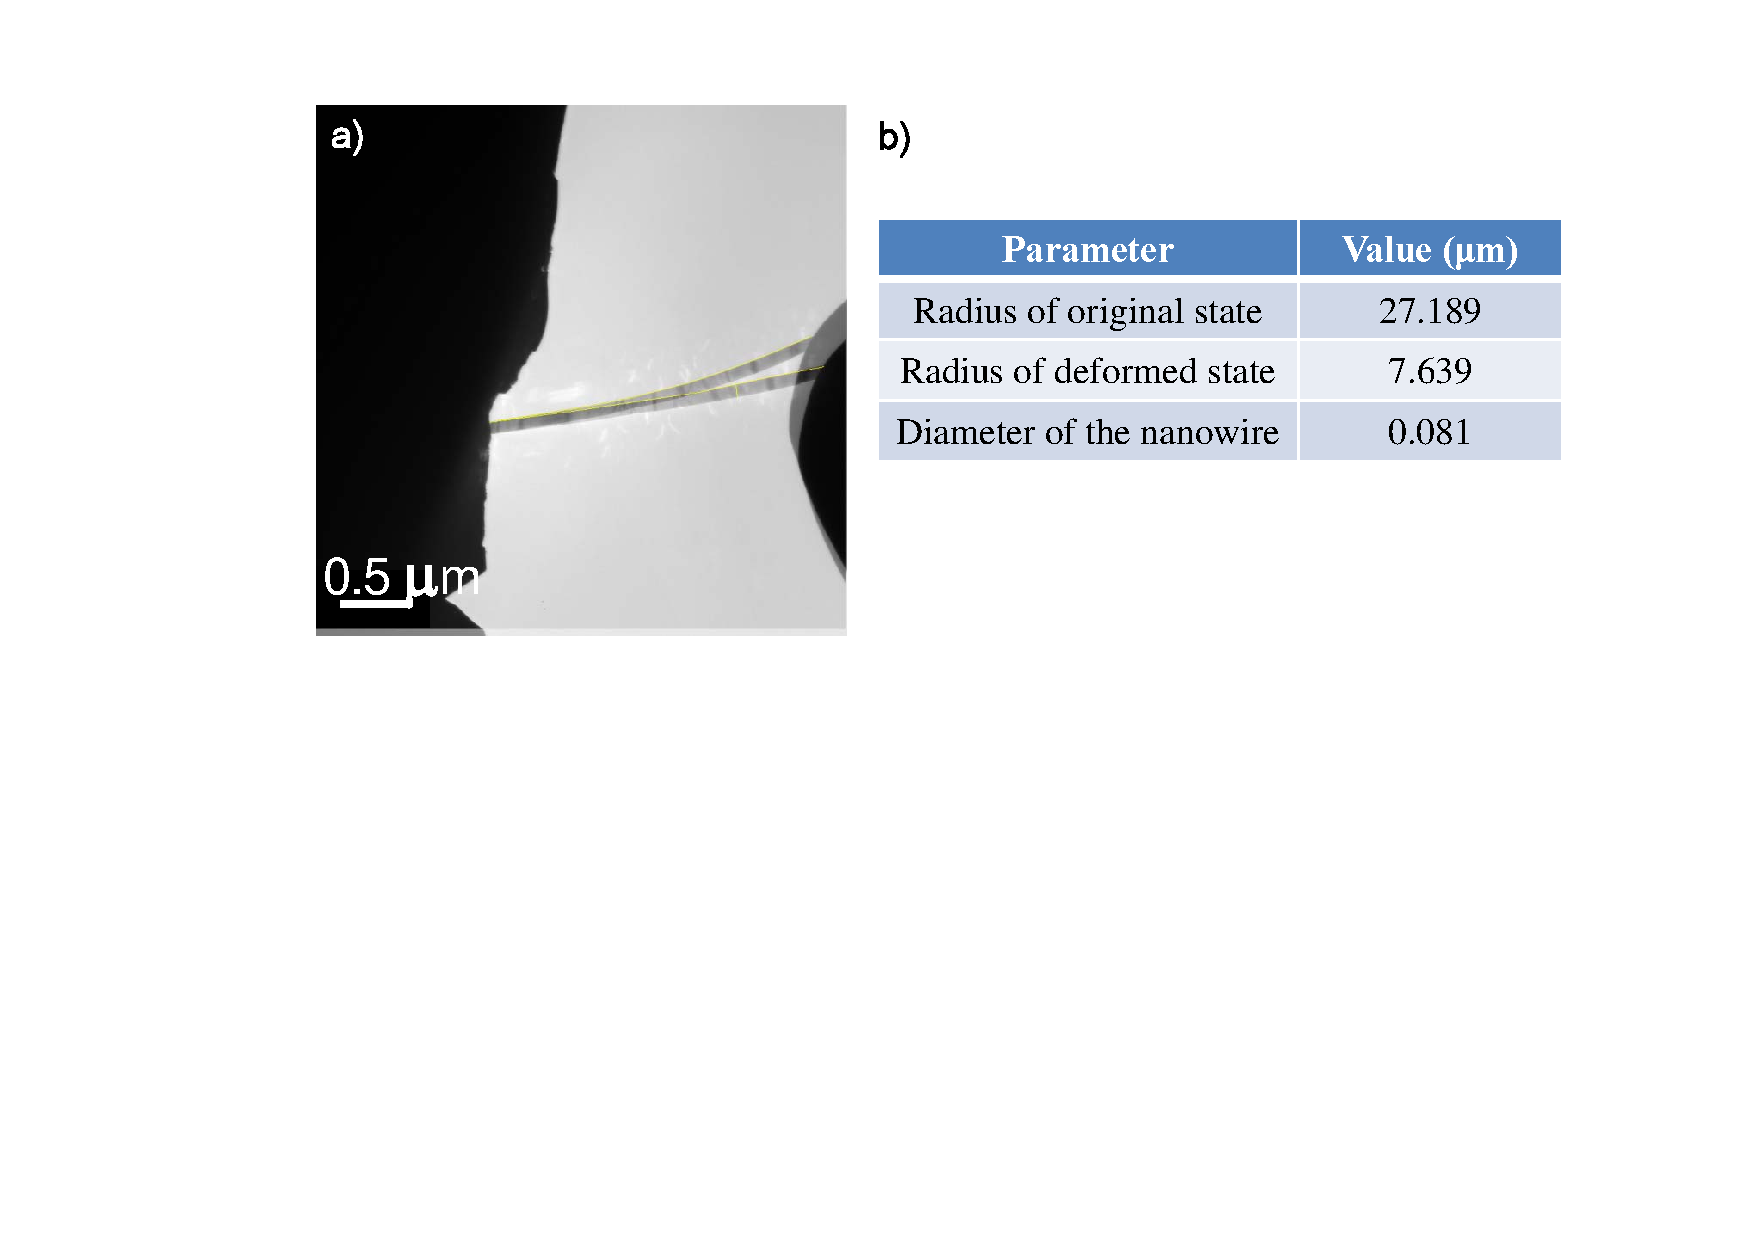
\includegraphics[height=\textwidth,angle=-90]{figures/figure6_s2}
\caption[Strain value]
{Strain values for an individual nanowire was determined under TEM imaging. 
(a) Two overlapped images of the nanowire in different states. 
(b) Measurements of the diameter of the nanowire, and its radius of curvature for the two cases. The strain was calculated as $d/R$, where $d$ and $R$ represent the diameter and the radius of curvature, respectively. The values were measured by using the {\em Digimizer} software\footnote{It is a free image analysis software from http://www.digimizer.com/}.
\label{fig:6_s2}}
\end{figure}

Two types of {\it in situ} experiments were conducted:\\
(1) Photocurrent I-V measurements, as illustrated in Figure \ref{fig:6_1} Scheme 1 in Chapter 2, while probing the I-V response of nanowires irradiated by a laser diode with a working wavelength of 488 nm. \\

(2) Photocurrent spectroscopy measurements, as described in Figure \ref{fig:6_1} Scheme 2 in Chapter 2, while measuring the wavelength dependency of the electrical current generated inside the nanowire under light illumination. 
The light source for photocurrent spectroscopy was a powerful laser driven light source (LDLS). The output of LDLS was then monochromated in order to carry out wavelength-selected measurements. 
In order to resolve the signal out of the noise, a chopper and a lock-in amplifier were applied in the measurement system. \\

\begin{figure}  [t]
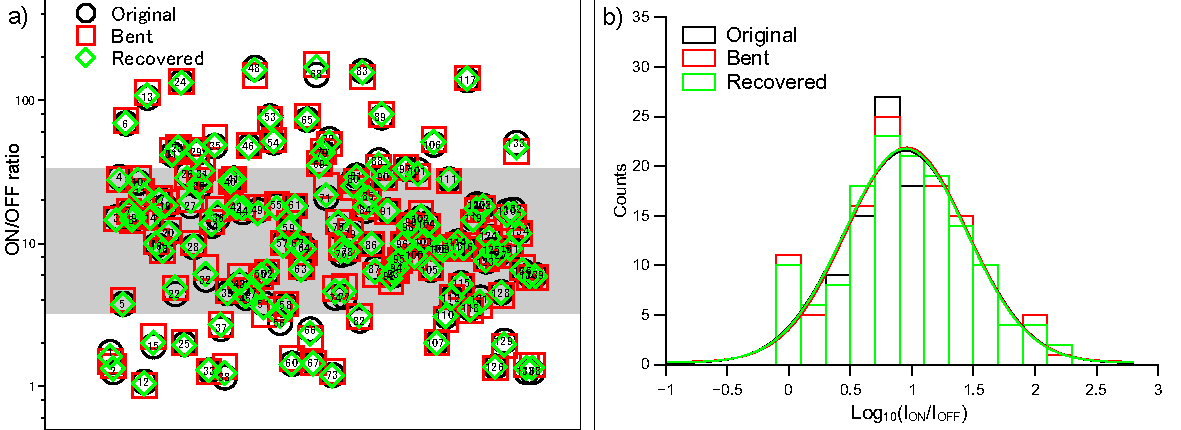
\includegraphics[width=\textwidth]{figures/figure6_3}
\caption[Statistical distribution of ON/OFF ratios]
{Statistical distribution of the measured ON/OFF (photocurrent/dark current) ratios for 139 bending/recovery experiments performed on free-standing single CdS nanowires. (a) ON/OFF ratios scatter mainly fits a gray region where the majority of measured ratios are included. (b) Statistical analysis of the ratios in log  scale. The lines represent Gaussian fits for the three histograms.
\label{fig:6_3}}
\end{figure}

\section{Results and discussions}
Photocurrents and dark currents of the nanowires were carefully measured by the sourcemeter before deformation, after it and after final and complete nanostructure recovery. 
Some of nanowires revealed stable contact properties during the deformations and recoveries, the other deviated from the stable behavior and possessed changed currents. 
Figure \ref{fig:6_2}a illustrates a contact to a nanowire in its original non-deformed state. \\

The average strain was defined as $\varepsilon = \frac{d}{R}$, where $d$ is the diameter of the nanowire, $R$ is its radius of  curvature.\footnote{Please not the the strain value determination here is the same as that in Chapter 5 in principle, but with a difference of constant factor of 2.} 
These two parameters were determined by a software, employing a curvature fit to the TEM images, as presented in Figure \ref{fig:6_s2} for a representative nanowire. 
I always try my best to get an intimate and stable physical contact, therefore the probe was slightly pressed towards the nanowire to avoid possible sliding between the probe and the specimen, as presented in Figure \ref{fig:6_2}a. 
The probe was then moved within the image plane for about 200 nm, leading to a strain of up to 1.68\%, as presented in Figure \ref{fig:6_2}b. 
The nanowire was finally recovered to its unbent state by moving the probe backwards, as illustrated in Figure \ref{fig:6_2}c. 
The I-V measurements were performed in both dark and illuminated conditions in each state, as summarized in Figure \ref{fig:6_2}d-e. 
In order to get a clear understanding of the correlation between the deformation states of the nanowires and the photocurrent responses, I performed numerous experiments for a comprehensive statistical analysis. 
The current values were found to be very much scattered. 
However, I found that the light ON/OFF ratio (photocurrent to dark current ratio) of the nanowires could be nearly stable. 

\begin{figure}[t]  
\centering
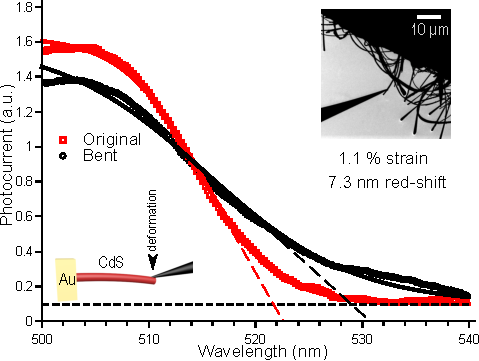
\includegraphics[width=250pt]{figures/figure6_4}
\caption[Photocurrent spectroscopy of deformed CdS NW]
{Photocurrent spectroscopy measurements performed on a representative individual CdS nanowire. The spectra have been fitted with logistic decay functions (solid lines); the regions of the curves corresponding to the symmetry point of each function have been extrapolated (dashed lines) to determine the intersections with the horizontal asymptote (dotted line). 
Left inset shows a schematic of the bending experiment. Right inset shows a low-magnification TEM image of the selected nanowire in contact with the W probe. 
\label{fig:6_4}}
\end{figure}

In this Chapter, I define three ON/OFF ratios, corresponding to the original, deformed and recovered states as:\\
{\center
$R_{ori} = \frac{I_{ph-ori}}{I_{dr-ori}}$, $R_{def} = \frac{I_{ph-def}}{I_{dk-def}}$, $R_{rec} = \frac{I_{ph-rec}}{I_{dk-rec}}$\\}

\vspace{5pt}, where $dk$ and $ph$ correspond to dark current and photocurrent, while $ori$, $def$ and $rec$ refer to the original, deformed and recovered states of the nanowire, respectively.\\

As presented in Figure \ref{fig:6_3}a, the values vary a lot for different cases. This might be caused by contact changes during probing, but the ON/OFF ratios are rather stable for each individual case. 
The statistical distributions of the ON/OFF values in Figure \ref{fig:6_3}b imply that this trend is valid in a wider scale and also allows us to estimate an average value of about 10, or around 7 to 20. 
The results of stable ON/OFF ratios made the majority of cases but some data had some deviations. 
Actually it is due to limitations of our setup with respect to the number of electrodes employed. These are only two. 
With only two electrical contacts, the contact resistance becomes an important uncertainty.\cite{Hummelgard2011} 
We expect that this variable could be reduced by the statistical analysis (on the basis that the contact resistance is normally randomly distributed). 
We expect that the nature of this variable (with respect to the resistance of the nanowire itself) allows for various contributions to be effectively separated. This enables us to observe the effects which are intrinsic to the nanowire samples themselves.

To get an additional information the photocurrent spectroscopy was performed under simultaneous TEM imaging. 

\begin{figure}  [t]
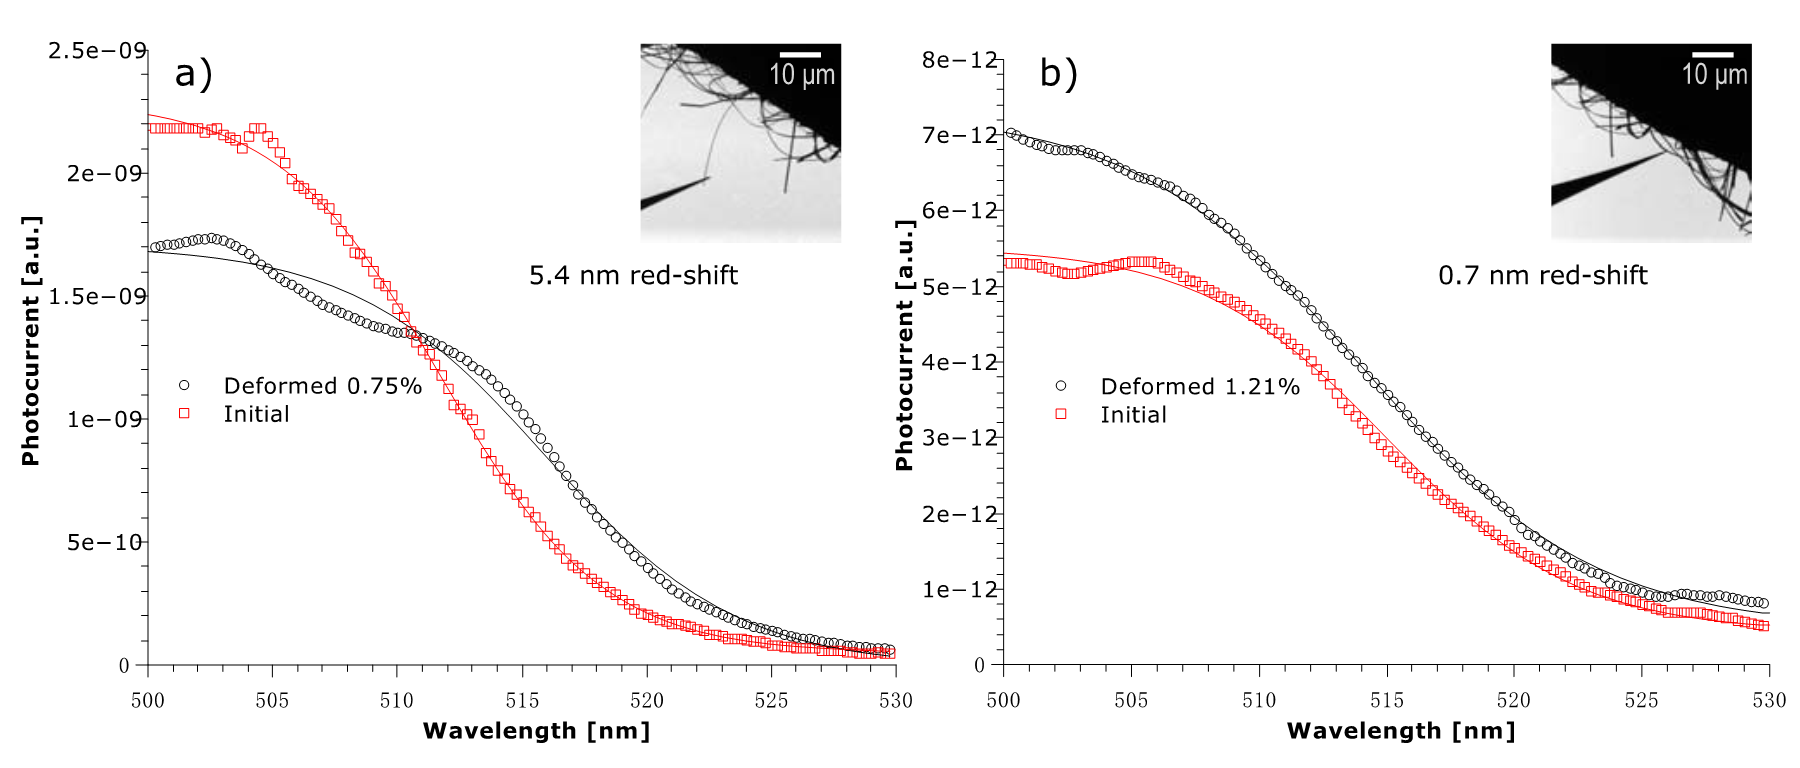
\includegraphics[width=\textwidth]{figures/figure6_s3}
\caption[Photocurrent spectroscopy of deformed CdS NW]
{(a,b) Additional examples of photocurrent spectroscopy on individual CdS nanowires, in their initial and deformed states. Low magnification TEM images are shown in the insets for each case. Strain and red-shift values are marked on each plot. 
\label{fig:6_s3}}
\end{figure}

In Figure \ref{fig:6_4}, the photocurrent spectroscopy results are plotted before and during the deformation process which introduces a 1.1\% elastic deformation.
The NW photocurrent cut-off wavelength possesses a 7.3 nm red shift under strain. At the initial state the edge wavelength was located at 521.8 nm. After deformation, the cut-off wavelength increased to 529.1 nm. 
More examples which feature similar red-shifts for the cut-off wavelength are shown in Figure \ref{fig:6_s3}. 
To sum up, the shifts of cut-off wavelength with regard to strains are listed in Table \ref{tab:6_1}. 

\begin{table}[b]
    \centering
    \begin{tabular}{c|c}
    \hline
         Strain (\%) & Red shifts (nm) (\%)\\
         \hline
         1.68 & 1.2\\
         0.75 & 5.4\\
         1.59 & -0.6\\
         1.21 & 0.7\\
         3.36 & 5.5\\
         \hline
    \end{tabular}
    \caption{Cut-off wavelength shift values for the independently deformed nanowires.}
    \label{tab:6_1}
\end{table}

Thus an average value of $3.3\pm2.9$ nm is obtained from Table \ref{tab:6_1}. The shift data shows that the effect is not limited to individual cases. 
The cut-off wavelength of the photocurrent spectrum is directly related to the electronic band structure. Thus it determines the near-band-edge emission (NBE) of the material. 
Our observations are consistent with the previous publications performed by measuring the CL of CdS nanowires inside SEM, where the authors observed red-shifted emission for the NBE peak under strain. 
This is an indication for a decrease in the bandgap value and it is in agreement with our data.\cite{Fu2011}

Evidence of the strain effects may cause the valence band decrease. Such strain effects may be observed by electron microscopy. 
Figure \ref{fig:6_5}ab presents the images of a CdS nanowire at the initial and deformed states. 
Insets of Figure \ref{fig:6_5}ab are SAED patterns from the area marked in Figure \ref{fig:6_5}ab. 

The averaged results presented here cannot accurately describe a single selected nanowire for its overall functional performance. 
In fact, the nanowires vary based on their morphology and structural peculiarities, even within the same synthetic batch of the material. 
There is a contradiction between the needs to accurately control the properties of every nanowire and the requirements for their high-yield production. However, from a statistical point of view, within a large number of structures, the nanowires studied here have common properties with respect to their photocurrent-to-dark current ratios. 


This means that the drawn conclusion is particularly important for devices fabricated by a large amount of nanowires (their bunches) instead of a single nanowire device. 
Some successful examples of making flexible photodetectors,\cite{Xu2015b} flexible transparent electrodes,\cite{Liu2014a} flexible supercapacitor electrodes,\cite{Liu2014a} LED arrays,\cite{Wang2015a} lithium-ion batteries,\cite{Wang2015} and solar cells,\cite{Zhang2012}, etc should be mentioned in this regard. \\

\begin{figure} [t] 
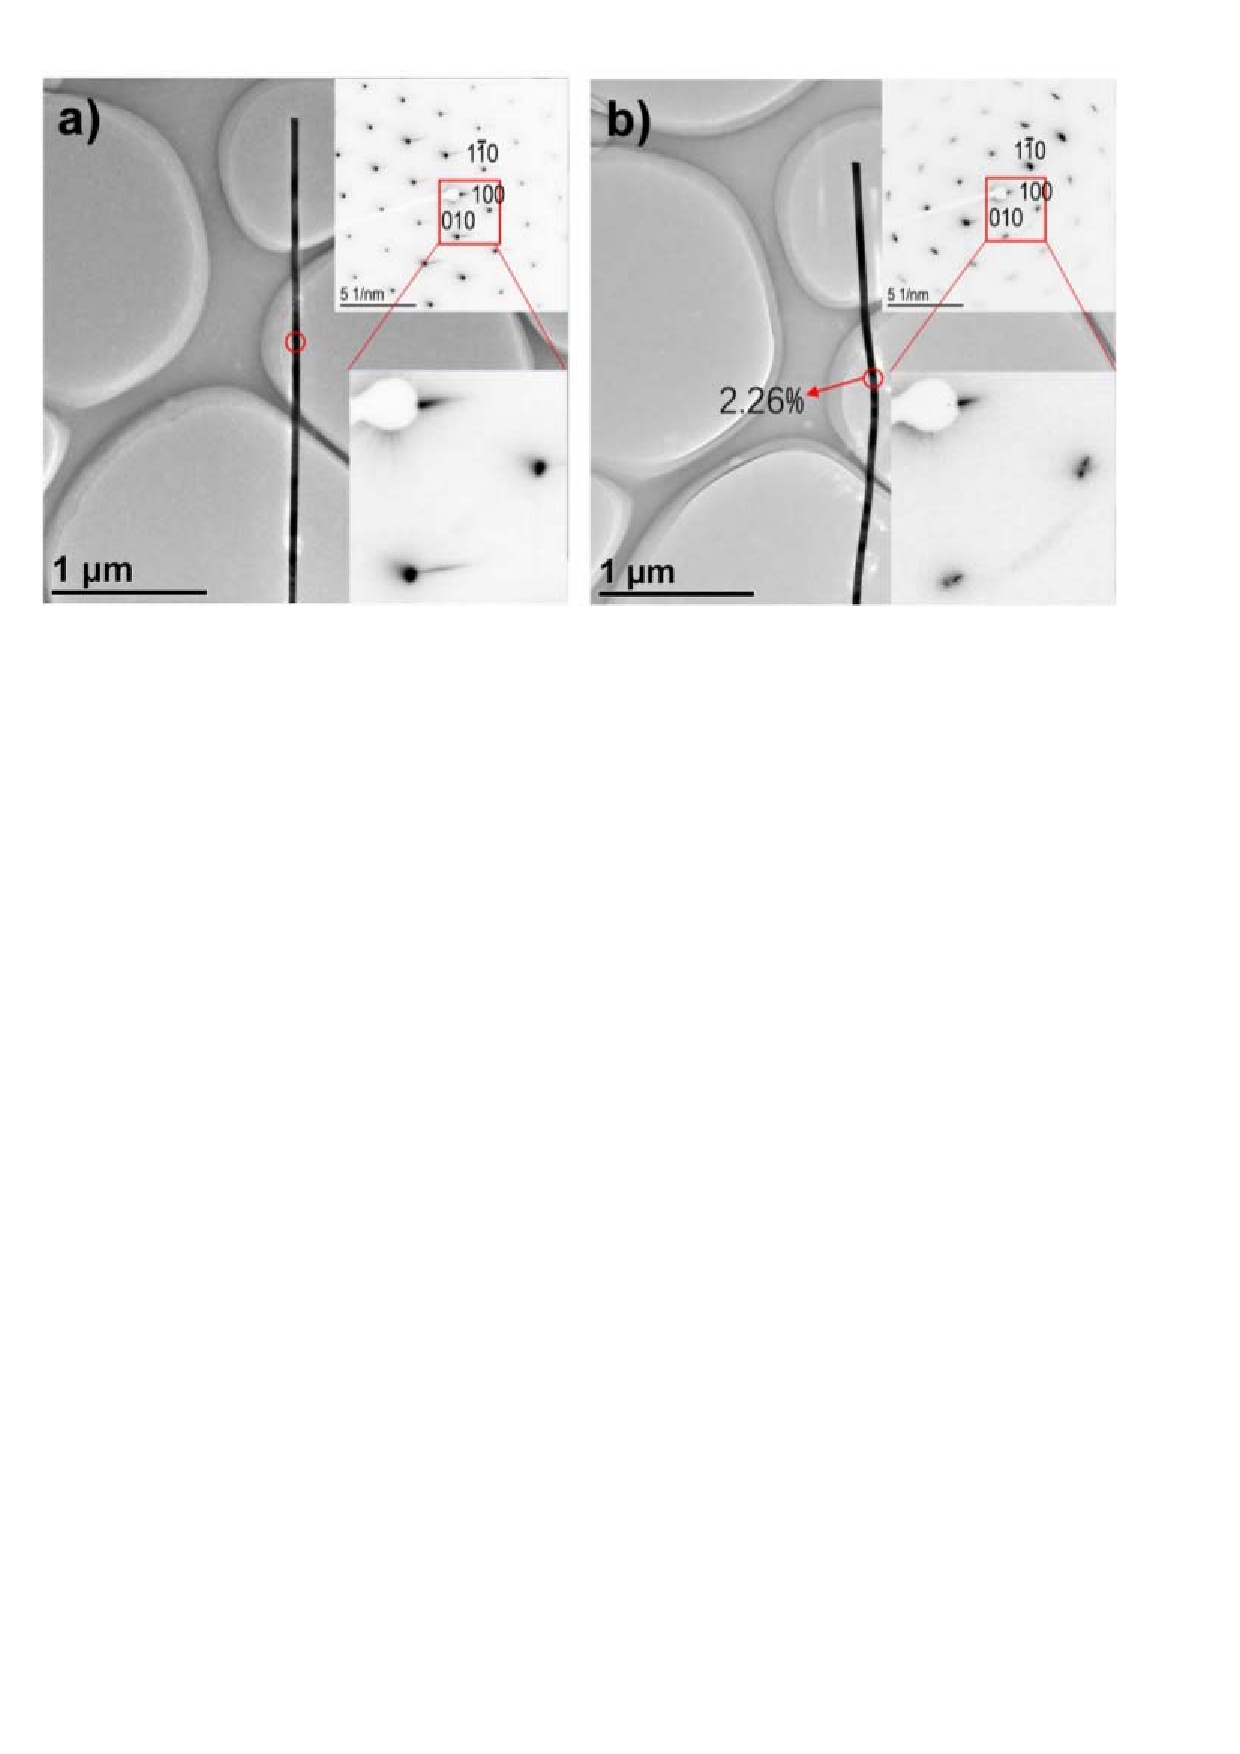
\includegraphics[width=\textwidth]{figures/figure6_5}
\caption[Diffraction of NW under strain]
{TEM images of the nanowire (a) before, and (b) after bending on a TEM carbon grid using a standard double-tilt holder due to the electron beam irradiation of the supporting C segments. 
The insets show SAED patterns along the [001] direction from areas marked by red circles. Representative framed parts of the SAED patterns are zoomed-in in the lower-right parts of the panels.
\label{fig:6_5}}
\end{figure}
\vfill


\section{Conclusions}
In conlusion, I have successfully performed photocurrent measurements for elastically deformed CdS nanowires inside the HRTEM. Using {\em in situ}  probing technique and the light illumination, I have characterized the electronic (dark current) and optoelectronic features of individual nanowires under mechanical deformation. 
To make the data reliable for future bottom-up applications, a large variety of nanowires was measured, which made possible an accurate statistical analysis of their properties. 
All nanostructures reveal fairly similar ON/OFF ratios in original, bent and recovered states, with this value mainly locating between 7 to 20. 
Photocurrent spectroscopy of several nanowires revealed red shifts of cut-off wavelength of several nanometers. 
These tiny shifts are mainly caused by deformation-induced strains, which induce changes in the electronic band structure. 
By taking SAED patterns, the strain induced structural deformation was vizualized after bending. 
The experiments reflect a variety of bending-induced stability features for individual nanowires. However, from a statistical point of view, the nanowires display common features in their response to deformation, making them highly valuable for future flexible optoelectronic applications. 


%update: Jan 15 fixed grammar according to prof notes.
%update: Jan 13 added a figure of solar cell. 
%update: Jan 09-11 prof check
%update: Dec 20 finished writing. 

%\begin{savequote}[75mm] 
%In three words I can sum up everything I've learned about life: it goes on.
%\qauthor{Robert Frost} 
%\end{savequote}

\chapter{Conclusions and Future Perspectives}

\newthought{In summary}, probing technique is applied to nanomaterials using \emph{in situ} TEM with many factors considered, such as chemical transitions, physical (electrical and mechanical) contacts and light illuminations. 
I reviewed and introduced related research in {\it in situ} probing TEM of nanomaterials for flexible optoelectronics and ion batteries applications in Chapter 1. 
Then the engineering details are discussed and presented in Chapter 2. 
Some behaviours or performances are revealed and discussed in Chapters 3-6, I finally summarize them herein and express my views of the future prospects based on my detailed understanding due to my PhD research experience. 

\section{Conclusions}
%chapter 3 revised
In Chapter 3, a direct and informative {\it in situ} probing \textit{nanoarchitectonics} technique to construct individual axial nanowire junctions has been for the first time realized. 
{\it In situ} HRTEM and in-tandem crystallography characterizations and optoelectronic behavior studies uncover the optical sensing properties of the single-crystalline axial CdS/p-Si nanowire junctions. 
The junctions exhibit decent selectivity toward the light wavelength shorter than those of the yellow range. 
It is very interesting that the junctions hold specific photocurrent saturation effect. 
The saturation of photocurrent at a relatively large bias could be utilized for the low power consumption light intensity sensing and integrated tunable voltage-driven devices, thanks to the corresponding current limitations and excellent tolerance toward some unreliable/unstable biases. 
Obviously, the present {\it nanoarchitectonics} approach employing {\it in situ} structural design and measurements gives hope for the timely establishing detailed operational principles of bottom-up nano-devices. \\

%chapter 4 revised
In Chapter 4, the designed phase-transformation route was found to be successful for fabrication of an N doped graphene-phosphorus anode material with layered sandwich-like morphologies where very thin amorphous red P layers are placed within flexible and conductive N-doped graphene frameworks.\\
Advantages of the as-designed anode material have been studied by various characterization techniques, device tests, {\it in situ} microscopy and theoretical calculations. 
These advantages are: \\
(1) Thin P layer on the doped graphene (instead of crystalline P) anode shows ultrastable efficiency of 0.002\% decay per cycle and good rate capability of 809 mAh/g at 1500 mA/g; \\
(2) P-C stable bonds may exist to tighly bind GN and P layers; \\
(3) {\it In situ} HRTEM experiments verified and revealed the reasons behind the ultrastable performance.\\

%chapter 5 revised
Chapter 5 discusses on the opto-mechano-electrical tripling phenomenon under {\it in situ} observation and probing measurements of photocurrents in zinc oxide nanowires in real time, and under high spatial resolution. 
By comparing photocurrent spectra of individual free-standing zinc oxide nanowires under strains, splitting of photocurrent spectra is established. 
The shifts of photocurrent peaks are in obvious correlation with the bending strains. 
The red/blue shifts are proved to be directly related to the splitting of energy levels in the valence band at $\Gamma$ point. 
DFTB calculations show a perfect match with the {\it in situ} probing experimental results. 
The splitting of photocurrent spectroscopy provides an important information for future flexible optoelectronics and piezo-phototronics. 
For example, this can be considered for strain tuned wavelength-division multiplexing modules or MOEMS devices, and for flexible optoelectronic components where photocurrent splitting value should be evaded as a key variable. \\

%chapter 6 revised
In Chapter 6, I have successfully performed photocurrent measurements for elastically deformed CdS nanowires inside the HRTEM. Using {\it in situ}  probing technique and light illumination, I have characterized the electronic (dark current) and optoelectronic features of individual nanowires under mechanical deformation. 
To make the data reliable for future bottom-up applications, a large variety of nanowires was measured, which made possible an accurate statistical analysis of their properties. 
All nanostructures reveal similar ON/OFF ratios in original, bent and recovered states, with a value mainly locating bwtween 7 and 20. 
Photocurrent spectra of several nanowires possess red shifts of cut-off wavelength of several nanometers. 
These tiny shifts are mainly caused by deformation induced strains, which result in the changes in the electronic band structure. 
By taking SAED patterns, the strain-induced structural deformation was confirmed after bending. 
The experiments reveal a variety of bending-induced stability for individual nanowires. However, from a statistical point of view, the nanowires display common features in their response to deformation, making them valuable for future flexible optoelectronic applications. \\

\section{Future perspectives}
%%%%%%%%%%%%%%%%%%%%%I guess this subsection is unnecessary%%%%%%%%%%%%%%%%%%%%%%%%%%%%%%%%%%
%\subsection{Look back to history to see where we are}
%Anthropologist believe that an evolution of mankind would be linked to the use of tools. \cite{lilley1948men} The ancients made tools to handle things at a meter scale, such as knife, wrench, scythe, sickle. Human civilization history is very much related to to development of tools. By updating tools, humankind was able to handle meter scale objects, and gradually went down to a few scales different from our size. The advancement of tools development is directly determined by the development of science and technology. 

%From millions of years ago, humankind started to updating tools. During prehistroy (before 3,000 BC) and ancient age (3,000 BC to 476 AC), more and more well the stones were machined, bronze and iron made tools came out to serve human beings for daily use - at a scale from centimeter to hundred of meters. In the paleolithic age, people were mainly making simple tools; while in the neolithic age, people became experienced with applying tools to building constructions. The capability of human beings are still restricted withing 3 scales from ourselves. It is called {\it meter-scale age}. 

%In the medieval age (476 AC to 1492 AC), the development of classical optics, including the production of well-made lenses, laid the groundwork for microscopy - the tool to reach microscale and astronomical scales. In modern age (1492 AC to 1789 AC), many revolutionary researches in optics and microscopy were associated and contributed to the fast development of physics, chemistry, biology and material science. It is called {\it micro-scale age}. 

%During the last century, development of particle physics, theory of relativity and quantum mechanics made it possible to see nanoscale world by electron microscopy and atomic force microscopy. It is called {\it nano-scale age}.

%The important mark between each "scale age" is the invention of an optical microscope and an electron microscope, because the preliminary important thing to do with the scale is to see objects in that scale. The main activities at the early stage of each "scale age" were development of the microscopy itself, as well as observing and getting knowledge of the new world objects. The main activities at the second stage of each "scale age" is the production of building blocks and their applications in those scales. Only when people become very familiar with almost everything in that scale with daily used applications, then science advances might move to the next scale via rising theories and making experiments. 

%After developing precised mechanics, humans became able to make fine mechanics to operate with the small objects. The gear was able to transfer a larger movement into fine movements. The ratio could be improved by the development of advanced gearing. However, it is not until recent years that people became capable to reach nanometer precision with mechanics once a piezoelectric motor has been invented. \cite{} 

%Clearly we are now in the cross road between the first stage and second stage of the {\it nanoscale age}. 

%%%%%%%%%%%%%%%%%%%abandoned paragraph, although I like it...%%%%%%%%%%%%%%%%%%%%%

\subsection{Nanoscale building blocks in future}
Although many researchers always claim that their nanomaterial samples are perfect and uniform, the quality is not that perfect to clarify on identical physical or chemical properties.\\

In Chapter 3, we noticed that the reproducibility (Table 3.1) is very high for heterojunctions with respect to the discovered saturation effect. 
But the current values vary a lot based on different sizes of building blocks. 
In Chapter 6, it is noticed that even the ratios of photo-to-dark current ratios in different states are more or less stable, the photo-to-current ratios of each nanowire are very different from each other. 
The scattered distribution of the ratios is caused by non-uniform structural features and chemical compositions. 
To use the nanowires in bundles is practical in some applications, while it is not practical to apply them in a single nanowire device for the mass production. \\

It is expected that nanoscale building blocks can be really uniform at the nanoscale. Such nanoscale building blocks become the bricks for the follow-up architecture. When the synthesis of various nanoscale building blocks can be well controlled to reach identical morphology, surface, physical, and chemical properties, the manufacturing process will become reliable and reproducible. \\

Another problem is that the current understanding of many nanomaterials is not yet comprehensive. But if the materials are synthesized with the identical morphology and crystallography, their properties are easier to be controlled. 

\subsection{Nanomanipulations in microscopy in the future}
We are now in 2017, the age of nanotechnology, gene engineering, information technology, artificial intelligence and many more striking discoveries. According to the history of tools, human beings are now quite new to the nanometer scale. The tools we are using for the nano-world are electron microscopy, atomic force microscopy, lithography, piezoelectric probing and other technologies. It is true that various nanostructures are indeed successfully synthesized these days, they may be designed on electronic chips for mass production, and their observations may be performed at the atomic resolution. However, lithography technology does not work for many other applications, microscopy has sampling limitations, mechanical technology is not mature yet to handle nanoscale building blocks easily. 

\begin{figure}  
\centering
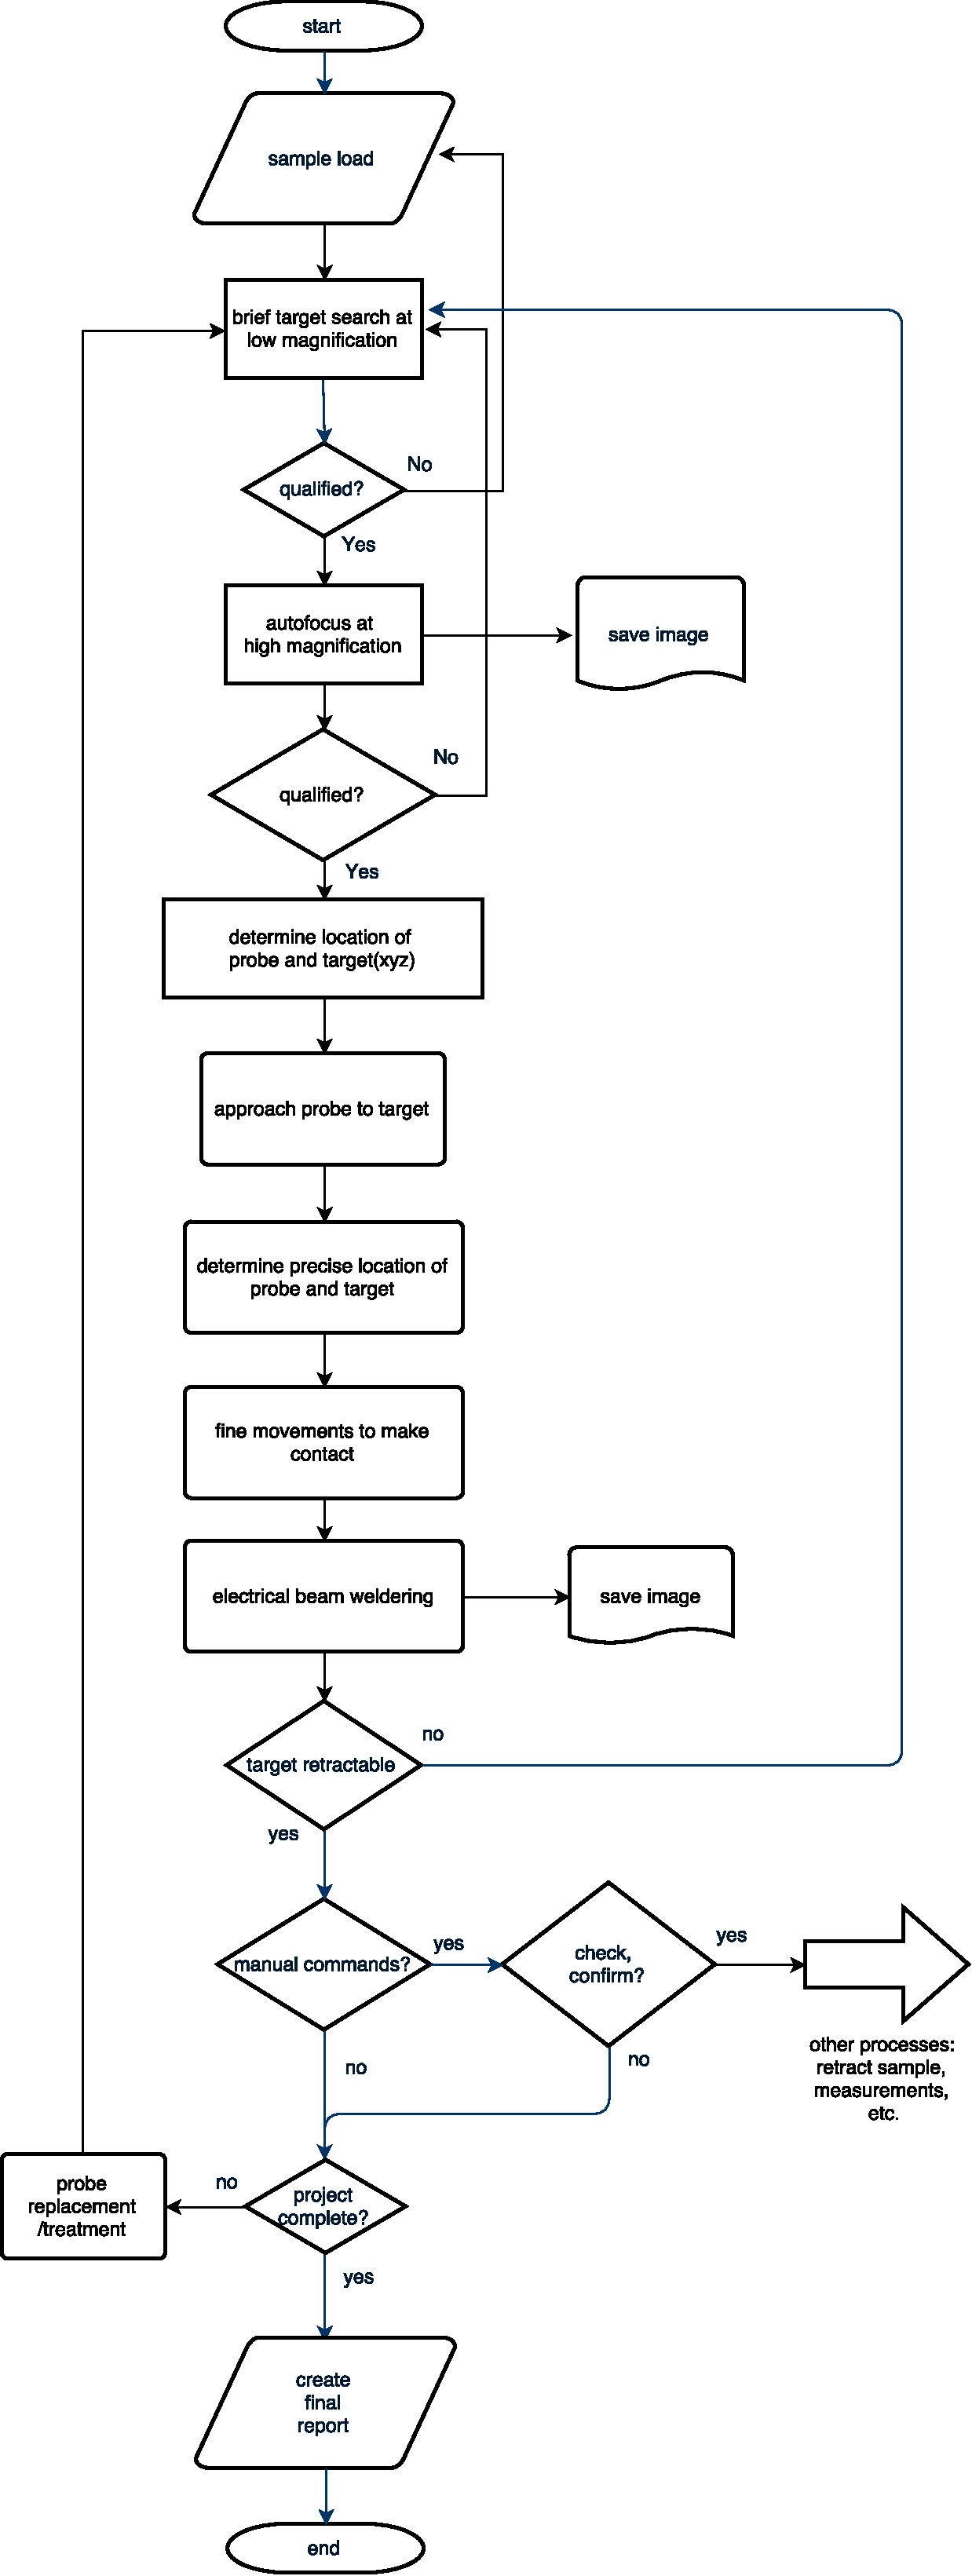
\includegraphics[width=236pt]{figures/figure7_ai}
\caption[Artificial intelligence for nanomanipulation]
{The workflow for nanoscale manipulations by automation.
\label{fig:7_aiworkflow}}
\end{figure}

During my research toward a PhD degree, I successfully performed thousands of nanoscale operations manually. Most processes are based on my personal experience.  
If we are able to translate our experience into codes for a machine, it is very possible that machines become able to perform the repeatable operations. In Figure \ref{fig:7_aiworkflow}, an example of automation of nanomanipulation is illustrated. In this workflow figure, the machine starts from sample loading, and then performs searching of qualified nanostructure targets, followed by automation of microscopy, second qualification check, autofocus and auto-alignment for high resolution imaging, third qualification check, determining location of probe and target sample, approaching and contacting probe to target, electron beam soldering, retracting a nanostructure target, and many other possible functions. 
Automation of nanoscale handling through SEM and AFM is also under research now. \cite{Fatikow1997Microsystem} We expect that automation will be mature for mass production of future micro- and nano-flexible optoelectronics based on bottom-up technology using various nanomaterials. 

\subsection{Nanomaterials for energy storage in the future}
Nanomaterials are superior in offering large surface to volume ratios, decent transport properties, variable physical parameters, and confinement effects owing to their nanoscale dimensions, and have been extensively studied for energy-related applications, such as solar cells, thermoelectrics, ion batteries, supercapacitors, and gas storage accumulators.\\
It is expected that the future energy storage is structurally designed down to nanoscale world to fully ultilize the nanodimensions -- as Feynman said, \textit{there is plenty of room at the bottom}. The volumetric capacity could be much higher, while at the same time the battery becomes stable and safe. \\
The problems may be solved through:\\
(i) generating optical effects to enhance the optical absorption in solar cells, \\
(ii) implementing a large surface area to boost the electrochemical reaction or molecular adsorption occurring at the solid–liquid or solid–gas interfaces, and\\
(iii) ensuring perfect crystallinity and/or porous structures to boost the electron or ion transport and electrolyte diffusion, so as to guarantee that the electrochemical process takes place with high efficiency. It is stressed that, in order to further optimize the capabilities of nanostructured materials for energy conversion and storage, new mechanisms and nanostructures are eagerly awaited. \\
In addition to highlighting the obvious advantages of nanostructured materials, their limitations and challenges for the usage in solar cells, lithium ion batteries, supercapacitors, and hydrogen storage systems are also required to be further investigated in all details.\cite{qifengzhang2013csr}\\


\begin{figure}  
\centering
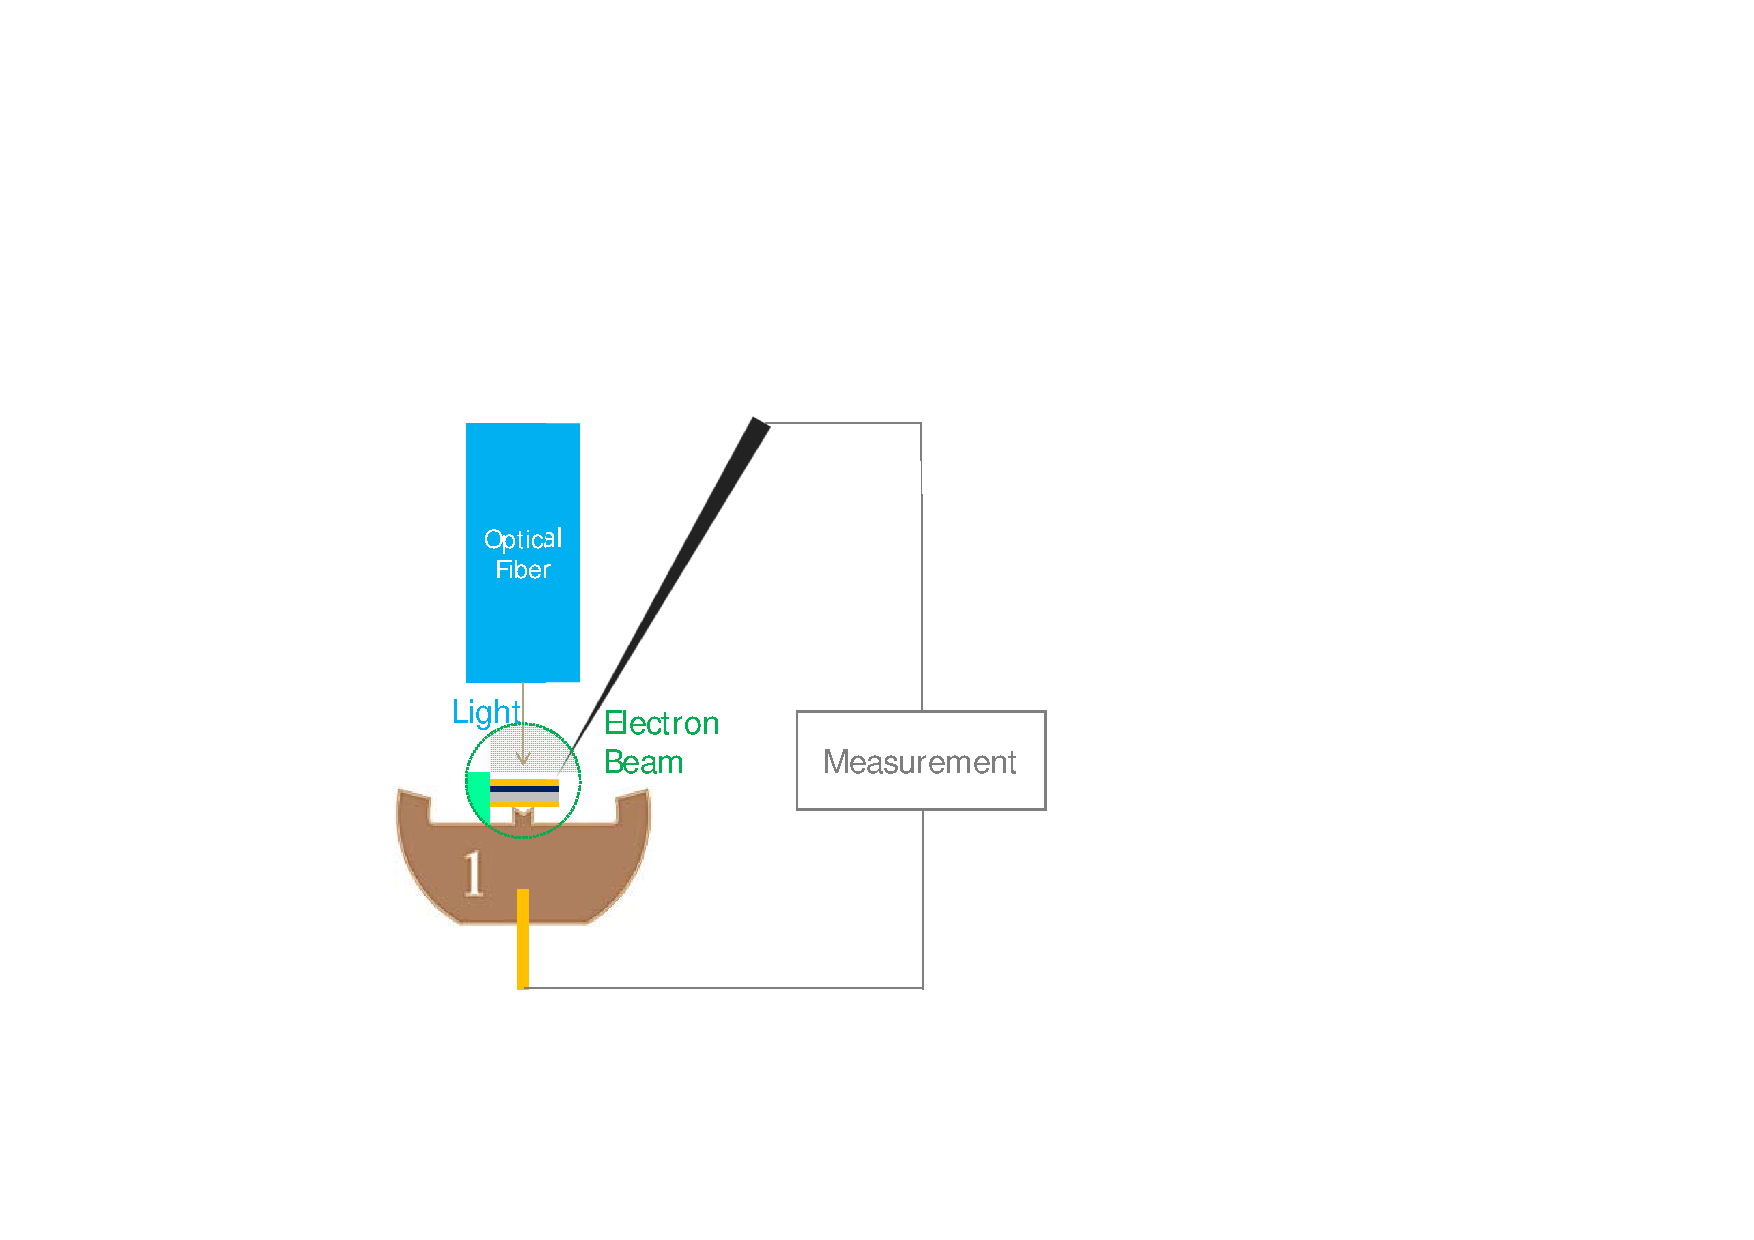
\includegraphics[height=300pt, angle=-90]{figures/figure7_sc}
\caption[\textit{In situ} solar cell]{\textit{in situ} TEM built solar cell. The layered specimen is prepared as a cross section of the solar cell.
\label{fig:7_sc}}
\end{figure}

\subsection{Nanoscale optoelectronics in the future}
All of us are expecting optoelectronics to be integrated into our daily life. To develop an integrated optical interconnect technology and to significantly decrease the energy consumption of future computing systems such paradigm could not be underestimated. The low-loss and high-speed features of optical interconnects would allow for the usage of much greater bandwidths. Taking electrical signals from processors and transferring them into optical/light signals, which are then transmitted \textit{via} optical waveguides on printed circuit boards, are the urgent steps. This is paving the way for integrating optical and electrical functions, as well as building components directly in the processors. \\
We probably would not get rid of silicon technology because it is still the best choice for microelectronics. However for an optical-electrical transfer, we require many semiconductors with different intrinsic electrical band structures. It is possible to integrate other materials, such as direct and wide band gap materials (such as CdS, ZnO), into silicon electronics. \\
Once the quality of these nanoscale building blocks becomes good enough (especially the present probably inconsistency is eliminated), once the nanoscale manipulation technology finds itself mature enough (mass automated production), the nanoscale optoelectronics should arrive at the real market. By simply placing several optoelectronic semiconducting nanoscale building blocks around a processor, optical-electrical signals within a single chip will first be applied to "green" and high-end computing, and then to our daily life necessities. 

%\subsection{Nanomaterials for flexible electronics in future}
%decide not to write this subsection

\subsection{\textit{In situ} probing TEM in the near future}
To creat pathways for future applications, experiments and investigations through \textit{in situ} microscopy are fundamental and essential. 

Various materials were tested using \textit{in situ} probing microscopy. Besides Si, CdS, P@GN and ZnO, as discussed in previous chapters, many other materials, such as \ce{TiO2} nanocrystals, \ce{MoS2} nanosheets, ZnSe/GaP nanowires and CdS/ZnO branched nanostructures also exhibited clear photocurrent responses, while \ce{SnO2@G} microsheets, Si/C nanospheres, \ce{Cu/Li4Ti5O12} scaffolds, \ce{MoS2/C} nanosheets and N doped graphene showed decent energy storage porfomances.\\

For electrical/optical \textit{in situ} probing TEM experiments, many other samples which I measured did not demonstrate strong photocurrent responses. For example, \ce{In2O3}, \ce{ZnS}, boron nitride(BN), \ce{BN-C}, \ce{BCNO}, \ce{CN} with wide/indirect band gap or low conductivity do not respond to the light illumination. For BN family materials, strong deep UV laser may excite carriers and lead to new results, but in my experiments, some regularly changing current signals were caused by absorbing light energy and heating. \\

Therefore, for the indirect band gap semiconductors, and for the not well-defined band gap materials, the electrical/optical \textit{in situ} probing TEM is not easy to detect possible small optoelectronic signals for various optoelectronic applications, but it is expected to do so in the future. It is also thought that the optical fiber plus electrical measuring equipments shall upgrade to collected and processed lower scale signals from smaller (regions of) samples. \\

As I mentioned in Chapter 2, \textit{in situ} photovoltage measurements are also possible to be performed by the similar microscopy setup. 

For instance, solar cells are not investigated in detail by \textit{in situ} TEM. One of my experimental designs for \textit{in situ} solar cell is presented in Figure \ref{fig:7_sc}. The solar cell can be processed by slicing and FIB and then placed in TEM. \\ 

For physical/chemical \textit{in situ} probing TEM experiments toward energy storage applications, the near future research is more clear, but still challenging. It is expected that the structure design would be more complicated and space-efficient taking care of higher-level control of structural consistency, and quality of the samples. The \textit{in situ} probing experiments for energy storage, including new types of ion-batteries (Aluminum-ion batteries and Magnesium-ion batteries), super-capacitors and some of the pseudocapacitors, are interesting directions which are anticipated. 



\singlespacing\clearpage\bibliographystyle{siam}\clearpage
\addcontentsline{toc}{chapter}{References}\bibliography{references} \clearpage
\addcontentsline{toc}{chapter}{Publications and presentations}

\chapter*{Publications \& Presentations}
\section*{Journal articles}
\noindent
\subsection*{2016}
%\years{2016}
\noindent1. {\underline {Zhang C.}}, Cretu O., Kvashnin D., Kawamoto N., Mitome N., Wang X., Bando Y., Sorokin P., Golberg D. "Statistically analyzed photoresponse of elastically bent CdS nanowires probed by light-compatible {\em in situ} High-Resolution TEM". {\em Nano Letters} 16(10), 6008-6013(2016); \\[5pt]
\noindent2. \underline{Zhang C.}, Wang X., Liang Q., Liu X., Weng Q., Liu J., Yang Y., Dai Z., Ding K., Bando Y. Golberg D. "Amorphous phosphorus/nitrogen-doped graphene paper for ultrastable sodium-ion batteries". {\em Nano Letters} 16(3), 2054-2060(2016);\\[5pt]
\noindent3. Xue Y., Dai P., Jiang X., Wang X., \underline{Zhang C.}, Tang D., Weng Q., Wang X., Pakdel A., Tang C. Bando Y., Golberg D. "Template-free synthesis of boron nitride foam-like porous monoliths and their high-end applications in water purification". {\em Journal of Material Chemistry A} 4(4), 1469-1478(2016);\\[5pt]
\noindent4. Hou G., Cheng B., Cao Y., Yao M., Li B., \underline{Zhang C.}, Weng Q., Wang X., Bando Y., Golberg D., Yuan F. "Scalable production of 3D plum-pudding-like Si/C spheres: Towards practical application in Li-ion batteries". {\em Nano Energy} 24, 111-120(2016); \\

\subsection*{2015}
%\years{2015}
\noindent5. \underline{Zhang C.}, Xu Z., Tian W., Wang X., Bando Y., Fukata N., Golberg D. “{\em In situ} fabrication and optoelectronic analysis of axial CdS/p-Si nanowire heterojunctions in a high-resolution transmission electron microscope”.{\em Nanotechnology} 26, 154001-8(2015);\\[5pt]
\noindent6. Xu Z., \underline{Zhang C.}, Bando Y., Bai X.D., Golberg D. “Lateral piezopotential-gated field-effect transistor of ZnO nanowires”. {\em Nano Energy} 13, 233-239(2015);\\[5pt]
\noindent7. Weng Q.H., Wang X., \underline{Zhang C.}, Jiang X., Bando Y., Golberg D. “Supercapacitive energy storage performance of molybdenum disulfide nanosheets wrapped with micoporous carbons”. {\em Journal of Material Chemistry A} 3, 3097-3102(2015); \\[5pt]
\noindent8. Wang. X, Liu D., Weng Q., Liu J., Liang X., \underline{Zhang C.} "Cu/Li4Ti5O12 scaffold as superior anode for lithium-ion batteries". {\em NPG Asia Materials} 7, 171(2015); \\[5pt]
\noindent9. \underline{Zhang C.}, Xu Z., Golberg D. " Opto-mechano-electrical tripling in ZnO nanowires probed by photocurrent spectroscopy in a high-resolution transmission electron microscope ".  {\em Applied Physics Letters} 107, 091103(2015); \\[5pt] 
\noindent10. Xue Y., Jiang B., Bourgeois B., Dai P., Mitome M., \underline{Zhang C.}, Yamaguchi M., Matveev A., Tang C., Bando Y., Tsuchiya K., Golberg D. "Aluminum matrix composites reinforced with multi-walled boron nitride nanotubes fabricated by a high-pressure torsion technique". {\em Materials \& Design} 88, 451-460(2015);\\[5pt]
\noindent11. Weng Q., Ide Y., Wang X.B., Wang X., \underline{Zhang C.}, Jiang X., Xue Y., Dai P., Komaguchi K., Bando Y., Golberg D. "Design of BN porous sheets with richly exposed (002) plane edges and their application as TiO2 visible light sensitizer". {\em Nano Energy} 16, 19-27(2015);\\[5pt]
\noindent12. Dai P., Xue Y., Wang X., Weng Q., \underline{Zhang C.}, Jiang X., Tang D., Wang X., Kawamoto N., Ide Y., Mitome M., Golberg D., Bando Y. "Pollutant capturing SERS substrate: porous boron nitride microfibers with uniform silver nanoparticle decoration". {\em Nanoscale} 7(45), 18992-18997(2015);\\

\subsection*{2014}
%\years{2014}
\noindent13. \underline{Zhang C.}, Tian W., Xu Z., Liu J., Li S., Tang D.M., Cai X., Wang X.,Weng Q., Liao M., Kawamoto N., Bando Y., Golberg D. “Photosensing performance of branched CdS/ZnO heterostructures as revealed by in situ TEM and photodetector tests”, {\em Nanoscale} 6, 8084-8090(2014);\\[5pt]
\noindent14. Golberg D., \underline{Zhang C.}, Xu Z. “Cubic lattice nanosheets: Thickness-driven light emission”, {\em ACS Nano} 8(7), 6516-6519(2014);\\[5pt]
\noindent15. Tian W., \underline{Zhang C.}, Zhai T., Li S.L., Wang X., Liu J., Jie X., Liu D., Lioa M., Koide Y., Golberg D., Bando Y. "Flexible ultraviolet photodetectors with broad photoresponse based on branched ZnS-ZnO heterostructure nanofilms”. {\em Advanced Materials} 26, 3088-3093(2014);\\[5pt]
\noindent16. Wang X., Weng Q.H., Liu X., Wang X.B., Tang D.M., Tian W., \underline{Zhang C.}, Yi W., Liu D., Bando Y., Golberg D. “Atomistic origins of high rate capability and capacity of N-doped graphene for Lithium storage”. {\em Nano Letters} 14, 1164-1171(2014);\\[5pt]
\noindent17. Wang X., Chen Z., Liu D., Tian W., Wang Q., \underline{Zhang C.}, Liu J.W., Han L., Bando Y., Golberg D. “Tripled-yolked ZnO-CdS hollow spheres for semiconductor-sensitized solar cells”, {\em Particle \& Particle Systems Characterization} 31(7), 757-762(2014);\\

\subsection*{Previously}
%\years{2012-2013}
\noindent18. Tian W., \underline{Zhang C.}, Wang X., Golberg D., Bando Y. “Flexible SnO2 hollow nanosphere film based high-performance ultraviolet photodetector”. {\em Chemical Communications} 49(36), 3739-3741(2013);\\[5pt]
\noindent19. Tian W., \underline{Zhang C.}, Wang X., Golberg D., Bando Y. "Flexible ultraviolet photodetectors with broad photoresponse based on branched ZnS-ZnO heterostructure nanofilms”. {\em Advanced Materials} 26(19), 3088–3093(2013);\\[5pt] 
\noindent20. Tian W. Wang X., Zhi C., Zhai T., Liu D., Zhang C., Golberg D., Bando Y. "Ni (OH)2 nanosheet@ Fe2O3 nanowire hybrid composite arrays for high-performance supercapacitor electrodes". {\em Nano Energy} 2(5), 754-763(2013).\\[5pt]
\noindent21. \underline{Zhang C.}, Huang H., Liang B., Wang X.F., Lan X., Xiang Q., Liu B., Chen D. "Patterned growth of In2O3 spheres organized by radially-aligned In2O3 nanobelts". {\em Journal of Nanoengineering and Nanomanufacturing} 2(2), 166-170(2012);\\[5pt]
\noindent22. Wang X.F., Huang H., Liu B., Liang B., \underline{Zhang C.}, Ji Q., Chen D., Shen G. "Shape evolution and applications in water purification: the case of CVD-grown Zn2SiO4 straw-bundles". {\em Journal of Material Chemistry} 22(12), 5330-5335(2012).\\

\section*{Oral presentations}

%\years{2016}
\noindent1. {\em Nanowire deformations and axial junction constructions in tandem with photocurrent measurements inside a transmission electron microscope}, MRS Spring 2016, Phoenix, USA(2016);\\[15pt]
%\years{2014}

\noindent2. {\em Optoelectronic properties of nanostructured materials as revealed by laser-compatible in situ Transmission Electron Microscopy}, 23rd Australian Conference on Microscopy and Microanalysis, Adelaide, Australia(2014). 

\section*{Poster presentations}
%\years{2016}
\noindent1. {\em Amorphous P@Graphene paper for ultrastable sodium-ion batteries}, AsiaNano 2016, Sapporo, Japan(2016);\\[15pt]
%\years{2015}
\noindent2. {\em In situ fabrication and photocurrent analysis of axial CdS/p-Si nanowire junctions by high-resolution TEM}, Japanese Society of Microscopy Kanto-branch meeting, Tokyo, Japan(2015). 



%\vspace{1cm}
\vfill{}
%\hrulefill\chapter*{Colophon}


\begin{center}

For my latest information of publications, please visit \\\url{https://scholar.google.com/citations?user=_tirUeIAAAAJ&view_op=list_works&sortby=pubdate}

Should you have any questions, please feel free to contact me by e-mail
\\\href{mailto:zhang.chao@nims.go.jp}{\nolinkurl{zhang.chao@nims.go.jp}} (until March 2017)
\\\href{mailto:zcelysium@gmail.com}{\nolinkurl{zcelysium@gmail.com}} (after March 2017)
\\[10ex]\emph{This is the end of the dissertation. } 

\end{center}

\end{document}
